\documentclass[12pt,openany,letterpaper]{mitthesis}

\pdfminorversion=4

\usepackage{lgrind}
\usepackage[margin=3cm]{geometry}
\usepackage[utf8]{inputenc}
\usepackage{colortbl}
\usepackage[spanish]{babel}
\usepackage{amsmath,mathrsfs}
\usepackage{etoolbox}
\usepackage{hyperref}
\usepackage{amsfonts}
\usepackage{amssymb}
\usepackage{dsfont}	
\usepackage{graphicx}
\usepackage{pdflscape}
\usepackage{afterpage}
\usepackage{cite}
\usepackage{footnote}
\usepackage{datatool}
\usepackage{pdfpages}
\usepackage{subfigure}

\usepackage{acronym}
\renewcommand{\bflabel}[1]{{\textbf{#1}\hfill}}
%\setlength\nomlabelwidth{1.5cm}
%\usepackage{nomencl}



\setlength{\parindent}{0pt}
%\setlength{\textwidth}{15cm}

% Replace parenthesis with (

\newcommand{\sortitem}[1]{%
  \DTLnewrow{list}% Create a new entry
  \DTLnewdbentry{list}{description}{#1}% Add entry as description
}
\newenvironment{sortedlist}{%
  \DTLifdbexists{list}{\DTLcleardb{list}}{\DTLnewdb{list}}% Create new/discard old list
}{%
  \DTLsort{description}{list}% Sort list
  \begin{itemize}%
    \DTLforeach*{list}{\theDesc=description}{%
      \item \theDesc}% Print each item
  \end{itemize}%
}

\makeatletter
\def\resetMathstrut@{%
  \setbox\z@\hbox{%
    \mathchardef\@tempa\mathcode`\[\relax
    \def\@tempb##1"##2##3{\the\textfont"##3\char"}%
    \expandafter\@tempb\meaning\@tempa \relax
  }%
  \ht\Mathstrutbox@\ht\z@ \dp\Mathstrutbox@\dp\z@}
\makeatother
\begingroup
  \catcode`(\active \xdef({\left\string(}
  \catcode`)\active \xdef){\right\string)}
\endgroup
\mathcode`(="8000 \mathcode`)="8000
%end

\hypersetup{
    bookmarks=true,         % show bookmarks bar
    unicode=false,          % non-Latin characters in Acrobat’s bookmarks
    pdftoolbar=true,        % show Acrobat’s toolbar?
    pdfmenubar=true,        % show Acrobat’s menu?
    pdffitwindow=true,     % window fit to page when opened
    pdfstartview={FitH},    % fits the width of the page to the window
    pdftitle={Solución a la indeterminación de las aberraciones producidas por un SLM y por sistemas ópticos en algoritmos de diversidad de fase},% title
    pdfauthor={Carlos Alfredo Cuartas Vélez},     % author
    pdfsubject={Trabajo de Grado},   % subject of the document
    %pdfcreator={Creator},   % creator of the document
    %pdfproducer={Producer}, % producer of the document
    pdfkeywords={Phase diversity} {Aberraciones} {Vórtices ópticos} {Modulador espacial de luz}, % list of keywords
    pdfnewwindow=true,      % links in new window
    colorlinks=true,       % false: boxed links; true: colored links
    linkcolor=blue,          % color of internal links (change box color with linkbordercolor)
    citecolor=red,        % color of links to bibliography
    filecolor=magenta,      % color of file links
    urlcolor=cyan           % color of external links
}

\pagenumbering{roman}

%\usepackage{fancyhdr}
%\pagestyle{fancy}
%\fancyhf{}
%\fancyhead[LE, RO]{\small \rightmark}
%\fancyhead[LO, RE]{\thepage}

\begin{document}

\renewcommand{\listfigurename}{Lista de Figuras}
\renewcommand{\listtablename}{Lista de Tablas}
\renewcommand{\contentsname}{Contenido}
\renewcommand{\tablename}{Tabla} 
\renewcommand{\bibname}{Referencias}

%%% Temas y subtemas tentativos en los capítulos
%
% Resumen 
%
% 1. Introducción
%  % Presentar objetivos
%
% 2. Vórtices ópticos
%  % Cargas topológicas fraccionales
%
% 2.1. Aberraciones ópticas
%
% 2.2. Moduladores espaciales de luz
%  % Twisted nematic % Parallel nematic  % Transmision % Reflexión
% 
% 3. Diversidad de fase
%  % PD tradicional % PD Coherente
%    IMAGENES
%	 Agregar aquí la parte de las aberraciones ópticas
%		
%
% 4. Implementación
%  % Generador de vortices % Generardor vortices con SLM real % 
%
% 5. Resultadoss
%
% 6. Conclusiones y trabajo futuro
%
% Referencias
%
%%%%

\author{Carlos Alfredo Cuartas Vélez}
\title{SOLUCIÓN A LA INDETERMINACIÓN DE LAS ABERRACIONES PRODUCIDAS POR UN MODULADOR ESPACIAL DE LUZ Y POR SISTEMAS ÓPTICOS EN ALGORITMOS DE DIVERSIDAD DE FASE.}

\newcommand\portada{
	\begin{titlepage}
		\begin{center}
			\vfill
			{\Huge \bf TRABAJO DE GRADO}
			\vfill
			{\large \bf Carlos Alfredo Cuartas Vélez\\
			ccuarta1@eafit.edu.co \par}
			\vfill
			{\normalsize \bf Universidad EAFIT \par}
			{\normalsize \bf Escuela de Ciencias \par}
			{\normalsize \bf Departamento de Ciencias Físicas \par}
			{\normalsize \bf Ingeniería Física \par}
			{\normalsize \bf Medellín, Colombia \par}
			{\normalsize \bf 2015\par}
		\end{center}
	\end{titlepage}
}

\newcommand\contraportada{
	\begin{titlepage}
		\begin{center}
			{\large \bf SOLUCIÓN A LA INDETERMINACIÓN DE LAS ABERRACIONES PRODUCIDAS POR UN MODULADOR ESPACIAL DE LUZ Y POR SISTEMAS ÓPTICOS EN ALGORITMOS DE DIVERSIDAD DE FASE} 
			\vfill
% 			{\large\bf PRESENTADO POR \par}
			{\large \bf CARLOS ALFREDO CUARTAS VÉLEZ} %Cód 201320001163}
			\vfill
			{\large Tesis de grado presentada como requisito parcial para optar al título de: \\ 
			\bf Ingeniero Físico\par}
			\vfill
			{\large\bf Director \par} 
                        {\large\bf PROF. RENÉ RESTREPO GÓMEZ \par}
                        
			\vfill
			{\normalsize \bf UNIVERSIDAD EAFIT \par}
			{\normalsize \bf ESCUELA DE CIENCIAS \par}
			{\normalsize \bf DEPARTAMENTO DE CIENCIAS FÍSICAS \par}
			{\normalsize \bf INGENIERÍA FÍSICA \par}
			{\normalsize \bf MEDELLÍN, COLOMBIA \par}
			{\normalsize \bf 2015\par}
		\end{center}
\end{titlepage}
}

\newcommand \aceptacion{
	\begin{flushleft}
		{\vspace*{3cm} \hspace{8cm} \normalsize Nota de aceptación \par}
		{\vfill \hspace{8cm} \hrulefill \par}
		{\vfill \hspace{8cm} \hrulefill \par}
		{\vfill \hspace{8cm} Asesor \par}
		{\vfill \hspace{8cm} \hrulefill \par}
		{\vfill \hspace{8cm} Jurado \par}
		{\vfill \hspace{8cm} \hrulefill \par}
		{\vfill \hspace{8cm} Jurado \par}
		{\vfill \hspace{8cm} \hrulefill \par}
		{\vfill \hspace{8cm} \normalsize Medellín, junio de 2015 \par}
		{\vspace*{3cm}}
	\end{flushleft}
}

\newcommand \dedicatoria{
	\begin{flushleft}
		{\vspace*{4cm} \hspace{8cm} \normalsize \textit{A mi familia, para que sea un} \par }
		{\hspace{8cm} \normalsize \textit{comienzo para todos ellos.} \par }
	\end{flushleft}
}

\newcommand \agradecimientos{
\chapter*{Agradecimientos}
	
	Quiero agradecer a mi familia, quienes siempre han estado conmigo para apoyarme a lo largo de toda mi vida y que tanto para mi como para ellos, es una experiencia enriquecedora. También, a compañeros por el apoyo durante la realización del proyecto. Asimismo al grupo de Óptica Aplicada de la Universidad EAFIT donde me he formado personal y profesionalmente, especialmente al profesor René Restrepo Gómez y a Santiago Echeverri con quienes he tenido la oportunidad de trabajar durante los dos últimos años y han compartido parte de su tiempo y conocimiento conmigo. Así como al profesor Luciano Ángel, quien mediante el proyecto ``Aberraciones ópticas en haces Laguerre-Gaussianos: corrección y aplicaciones metrológicas'', además de dar el primer paso para la realización de este trabajo, permitió mi vinculación con el grupo de investigación. Por último, agradecer a la Universidad EAFIT, en especial a la beca ANDI, quienes son los responsables de la oportunidad que tuve de emprender este camino. 
}

\newcommand \resumen{
\chapter*{Resumen}
%La óptica singular es una rama de la óptica que se desarrolla hace relativamente poco. Con la aplicación de vórtices ópticos para problemas tales como micromotores su estudio ha incrementado en los recientes tiempos. Uno de los problemas más comunes con los vórtices ópticos es su sensibilidad ante cierto tipo de aberraciones de primer orden. Las aberraciones pueden provenir de diversas fuentes, tales como los elementos empleados en el sistema óptico así. En los últimos años con el desarrollo de los cristales líquidos y los hologramas generados por computadora, es más común encontrar que se emplean moduladores espaciales de luz como objetos de fase que otorgan sus características a los OVs. Ahora si bien es cierto que emplear SLMs tiene sus ventajas (por ejemplo, posibilidad de generar OVs de diferentes cargas topológicas), también es cierto que cuando los SLMs son de baja calidad, estos también pueden deformar los OVs que producen. El grupo de Óptica Aplicada de la Universidad EAFIT ha estado trabajando no solo en la generación de OVs, si no que además han desarrollado un método para caracterizar las aberraciones que estos puedan presentar. Este método se ha basado en el concepto de diversidad de fase, que es una técnica iterativa de recuperación de aberraciones en sistemas incoherentes. La aplicación de PD a OVs a traído con sigo una nueva posibilidad para la caracterización de las aberraciones que inducen los SLM de baja calidad, esto basado en el conocimiento profundo del SLM. Por ello, en este proyecto se plantea un método para recuperar y discernir la contribución de las aberraciones causadas por un sistema ópticos y las causadas por un SLM de transmisión. \\

%En este trabajo se presentan los resultados de modificar los algoritmos de diversidad de fase propuestos por el grupo de Óptica Aplicada de la Universidad EAFIT, de forma que es posible discernir las aberraciones causadas por la modulación en fase de un modulador espacial de luz (SLM) de transmisión y las aberraciones causadas por el sistema óptico.

%En este trabajo se presenta una modificación a los algoritmos de diversidad de fase, para la recuperación de aberraciones en sistemas ópticos, propuestos por el grupo de óptica aplicada de la universidad EAFIT. Estas modificaciones permiten identificar de manera independiente, las aberraciones ocasionada por la modulación en fase de un modulador espacial de luz (SLM) y aquellas ocasionadas por los demás elementos ópticos.

En este trabajo se presenta una modificación a los algoritmos de diversidad de fase coherente, propuestos por el grupo de óptica aplicada de la Universidad EAFIT. A través de dichos algoritmos, es posible recuperar las aberraciones de un sistema óptico, empleando vórtices ópticos generados con un modulador espacial de luz. Aunque las aberraciones sean recuperadas, su fuente no es predicha por diversidad de fase coherente, es por ello, que se proponen dos modificaciones que permiten discernir la procedencia de éstas.\\

%En primera instancia, se obtiene una caracterización de la modulación en fase y amplitud del SLM y se plantea un nuevo esquema para la simulación de vórtices ópticos generados en un sistema limitado por difracción, empleando las características experimentales del SLM.\\

Las modificaciones sobre diversidad de fase, se basan en el empleo de la curva de modulación de fase del modulador espacial de luz, por lo tanto, en primera instancia, se obtiene una caracterización del modulador espacial de luz. En particular, se analiza la generación de vórtices ópticos para tres curvas de modulación, y desde este análisis, se propone un nuevo esquema para la simulación de vórtices ópticos, propagados por un sistema limitado por difracción con la modulación de fase experimental. La adición de este elemento, permite proponer una nueva variable de entrada para diversidad de fase coherente, con lo cual, se efectúan las modificaciones propuestas.\\

También se obtienen los resultados experimentales de las aberraciones, se realiza una comparación de aquellas recuperadas con diversidad de fase coherente, y sus respectivas modificaciones. Con base en los resultados obtenidos, se concluye que es posible discernir la fuente de las aberraciones, y obtener una corrección de manera independiente.}

%En este trabajo, se obtienen los resultados experimentales de las aberraciones propuestas, y también se realiza una comparación de aquellas recuperadas con diversidad de fase coherente, y sus respectivas modificaciones. De esto, se obtiene que efectivamente es posible discernir, tanto las aberraciones, como la fuente de estas, y obtener una corrección de manera independiente.}

%Las modificaciones propuestas se basan en el empleo de la curva de modulación experimental del SLM, de forma que la información de las aberraciones causadas por la modulación en fase del SLM sea incluida en el esquema de diversidad de fase. A partir de esto es posible modificar los parámetros de entrada para diversidad de fase y debido a esto, las aberraciones encontradas por el algoritmo corresponderán, o bien a las causadas solo por la modulación en fase, o por el sistema óptico.\\

%En este trabajo también se realiza la corrección de las aberraciones de forma individual para luego obtener la aberración de la modulación en fase del SLM a partir de las aberraciones totales y las aberraciones recuperadas para el sistema óptico.}

%\textbf{Palabras claves:} vórtice óptico, diversidad de fase, modulador espacial de luz, aberraciones ópticas.
%}

\portada 
\thispagestyle{empty}

\newpage\null\thispagestyle{empty}\newpage

\contraportada
\thispagestyle{empty}
\newpage\null\thispagestyle{empty}\newpage

\aceptacion
%\thispagestyle{empty}
\newpage
\newpage\null\thispagestyle{empty}\newpage

\dedicatoria
\newpage\null\thispagestyle{empty}\newpage

%\thispagestyle{empty}
\newpage
\agradecimientos
\addcontentsline{toc}{section}{\bf Agradecimientos}
\newpage
\newpage\null\thispagestyle{empty}\newpage

%\thispagestyle{empty}
\newpage
\resumen
\addcontentsline{toc}{section}{\bf Resumen}
\newpage
\newpage\null\thispagestyle{empty}\newpage


\tableofcontents
%\thispagestyle{empty}
\newpage
\listoffigures
%\thispagestyle{empty}
\newpage
\listoftables
%\thispagestyle{empty}
\newpage

\addcontentsline{toc}{section}{\bf Lista de acrónimos}
\chapter*{Lista de acrónimos}
\begin{acronym}[AWGN]
%\acro{Fig}{Figura.}
\acro{OV}{Vórtice óptico.} 
\acro{OAM}{Momento angular orbital.}
\acro{LC}{Cristal líquido.} 
\acro{SLM}{Modulador espacial de luz.} 
\acro{PD}{Diversidad de fase.}
\acro{GSA}{Algoritmo de búsqueda de gradiente.} 
\acro{CMR}{Curva de modulación real.} 
\acro{TN-LCD}{Pantalla de cristal líquido \textit{twisted nematic}.} 
\acro{CGH}{Holograma generado por computadora.} 
\acro{SPP}{Placa de fase espiral.}
\acro{SPM}{Máscara de fase espiral.} 
\acro{WFS}{Sensor de frente de onda.} 
\acro{PSF}{Función de punto extendido o función de dispersión de punto.} 
\acro{OTF}{Función de transferencia óptica.}
\acro{FT}{Transformada de Fourier.}
\acro{GP}{Pupila generalizada.} 
\acro{CTF}{Función de transferencia coherente.} 
\acro{PD1}{Diversidad de fase modificación 1: Sensor de aberraciones por elementos ópticos diferentes al SLM.} 
\acro{PD2}{Diversidad de fase modificación 2: Sensor de aberraciones por la modulación de fase del SLM.} 
\acro{HWP}{Lámina retardadora de media longitud de onda ($\lambda /2$).}
\acro{QWP}{Lámina retardadora de un cuarto de longitud de onda ($\lambda /4$).} 
%\acro{P}{Polarizador.} 
\acro{PSG}{Generador de estados de polarización.} 
\acro{PSA}{Analizador de estados de polarización.} 
\acro{RMS}{Media cuadrática.} 
\acro{RD}{Red de difracción.} 
\acro{TEM}{Modo transversal electromagnético.} 
\end{acronym}
\newpage

%\section*{Notación}
%\begin{acronym}[AWGN]
%
%\acro{$(x,y)$}{Coordenadas espaciales.}
%\acro{$(r,\theta)$}{Coordenadas polares.}
%\acro{$(\xi,\eta)$}{Coordenadas frecuenciales.}
%\acro{$\vec{x}$}{Vector de posición bidimensional. Representa las coordenadas $(x,y)$.}
%\acro{$\vec{u}$}{Vector de frecuencias bidimensional. Representa las coordenadas $(\xi,\eta)$.}
%\acro{$\psi_l$}{Función que representa la distribución de fase de un vórtice óptico de carga topológica $l$.}
%\acro{$l$}{Carga topológica.}
%\acro{$\hbar$}{Constante de Planck normalizada.}
%\acro{$i$}{Unidad imaginaria.}
%\acro{$\phi$}{Fase de una onda bidimensional.}
%\acro{$LG_{l,p}$}{Modos Laguerre-Gauss con índices de variación azimutal y radial, $l$ y $p$ respectivamente.}
%\acro{$w$}{Ancho de un haz Gaussinao.}
%\acro{$L_p^{|l}$}{Polinomios asociados de Laguerre.}
%\acro{$q$}{Órdenes de difracción.}
%\acro{$d(\vec{x})$}{Plano imagen para un sistema con iluminación incoherente.}
%\acro{$d_{obj}(\vec{x})$}{Plano objeto para un sistema con iluminación incoherente.}
%\acro{$s(\vec{x})$}{Función de punto extendido (PSF).}
%\acro{$\otimes$}{Operador convolución.}
%\acro{$\mathscr{F}$}{Transformada de Fourier.}
%\acro{$D(\vec{u})$}{Transformada de Fourier de $d(\vec{x})$.}
%\acro{$D_{obj}(\vec{u})$}{Transformada de Fourier de $d_{obj}(\vec{x})$.}
%\acro{$S(\vec{u})$}{Función de transferencia óptica (OTF).}
%\acro{$H(\vec{u})$}{Función de transferencia coherente (OTF).}
%\acro{$\star $}{Operador autocorrelación.}
%\acro{$h(\vec{x})$}{Función respuesta al impulso o PSF de amplitud.}
%\acro{$A$}{Función de tramitancia de la pupila.}
%\acro{$j$}{Índice de las diversidades de aberración.}
%\acro{$L$}{Funcional de minimización.}
%\acro{$(m,n)$}{Píxeles en una imagen.}
%\acro{$Z_n^m$}{Polinomios de Zernike de orden radial $n$ y azimutal $m$.}
%\acro{$R_n^m$}{Función de variación radial de los polinomios de Zernike.}
%\acro{$G^m$}{Función de variación azimutal de los polinomios de Zernike.}
%\acro{$\delta$}{Delta de Kronecker.}
%\acro{$W$}{Frente de onda.}
%\acro{$a_i$}{Vector de pesos en la base de Zernike}
%\acro{$u(\vec{x})$}{Campo imagen para un sistema con iluminación coherente.}
%\acro{$u_{obj}(\vec{x})$}{Campo objeto para un sistema con iluminación coherente.}
%\acro{$U(\vec{u})$}{Transformada de Fourier de $u(\vec{x})$.}
%\acro{$U_{obj}(\vec{u})$}{Transformada de Fourier de $u_{obj}(\vec{x})$.}
%\acro{$\phi_{coh}$}{Aberración recuperada mediante el algoritmo de diversidad de fase.}
%\acro{$\phi_{so}$}{Aberración del sistema óptico sin el SLM.}
%\acro{$\phi_{slm}$}{Aberración causada por la modulación en fase del SLM.}
%\acro{$\omega_{1,2,3}$}{Estados de polarización para la generación de OVs.}
%\end{acronym}
%\newpage
\pagenumbering{arabic}

\chapter{Introducción}
\label{cap:introduccion}

%Las singularidades son puntos de magnitud indeterminada que se presentan en diversos sistemas físicos \cite{Dennis2009}; por ejemplo, si tomamos un imán y analizamos las líneas de campo, estas deben cerrarse sobre el imán, pero en el caso de los polos, la dirección del campo no se encuentra definida. Un vórtice óptico (OV: \textit{optical votex}) es una singularidad que ocurre en la fase de un haz y se da por la presencia de momento angular orbital (OAM: \textit{orbital angular momentum}) en los fotones \cite{Uribe2011, Cheng2013}. Cuando se tiene un haz con OAM diferente de cero, la fase rota al rededor de un eje perpendicular al plano objeto en la dirección de la propagación, describiendo una helicoide, y la intensidad del haz se desvanece en el centro a causa de la singularidad.\\

Las singularidades son puntos de amplitud nula y de fase indeterminada que se presentan en diversos sistemas físicos \cite{Dennis2009}; por ejemplo, si tomamos un imán y analizamos las líneas de campo, éstas deben cerrarse sobre el imán, pero en el caso de los polos, la dirección del campo no se encuentra definida. Un vórtice óptico (OV: \textit{optical vortex}) es una singularidad que se presenta en la fase de un haz, y se da por la presencia de momento angular orbital (OAM: \textit{orbital angular momentum}) en los fotones \cite{Uribe2011, Cheng2013}. Cuando se tiene un haz con OAM diferente de cero, la fase rota perpendicularmente respecto a un eje en la dirección de propagación, describiendo un helicoide, y la intensidad se desvanece en el centro del haz a causa de la singularidad de fase.\\

%Para generar OVs se requiere modificar la distribución de fase usando las conocidas máscaras espirales \cite{Rozas1999, Bazhenov1990}; para ello se han empleado elementos como placas de fase espiral \cite{Ruffato2014, Schemmel2014} o redes de difracción \cite{Bekshaev2010, Heckenberg1992, Bekshaev2010a}, aunque gracias a los avances en cristales líquidos (LCs: \textit{liquid crystals}) y los hologramas generados por computadora, la forma más común de generar OVs es a través de un modulador espacial de luz (SLM: \textit{spatial ligth modulator}). Estos últimos son dispositivos opto-electrónicos que modifican la amplitud o la fase de la luz de forma controlada empleando LCs \cite{Uribe2011, Burman2010, Gennes2007}.\\

Una forma de generar OVs consiste en la modificación de la de fase en un haz Gaussiano, de forma que se impone una distribución en espiral a la fase del haz\cite{Rozas1999, Bazhenov1990}. Para obtener una distribución de fase espiral, se han empleado dispositivos tales como: placas de fase espiral \cite{Ruffato2014, Schemmel2014} o rejillas de difracción \cite{Bekshaev2010, Heckenberg1992, Bekshaev2010a}. Aunque, gracias a los avances en cristales líquidos (LCs: \textit{liquid crystals}) y los hologramas generados por computadora, se ha visto potenciado el empleo de moduladores espaciales de luz (SLM: \textit{spatial light modulator}) para la generación de OVs. Estos últimos, son dispositivos opto-electrónicos que modifican la amplitud o la fase de la luz de manera controlada, para ello, emplean las propiedades de los LCs \cite{Uribe2011, Burman2010, Gennes2007}. Cuando un campo definido por una amplitud con distribución Gaussiana y un frente de onda plano, se propaga a través de una lente, se esperaría obtener un disco de Airy en el plano focal, por otro lado, cuando la fase de la distribución Gaussiana posee una vorticidad óptica, en el plano focal se obtiene una distribución de intensidad toroidal propia de los OVs.\\


%Para obtener Ovs se han empleado placas de fase espiral, redes de difracción, . Pero con el desarrollo de los cristales líquidos y los hologramas generados por computadora, en los últimos años se han empleado moduladores espaciales de luz como generadores de chgs. Un SLm es un dispositivo opto-electrónico que permite modificar las propiedades de un haz, bien sea la amplitud o la fase.

%que se presentan en diversos sistemas físicos, en donde se da una indeterminación en la magnitud del campo. Un vórtice óptico es en una singularidad que ocurre en la fase de un haz de luz, este aparece gracias a la presencia de momento angular orbital. Cuando se tiene un haz con oam distinto de cero, entonces en la intensidad se obtiene una estructura que posee su núcleo oscuro, es decir, la luz se distribuye alrededor del centro, pero este permanece oscuro. Cuando se generan a través de un sistema óptico, es de esperar que al igual que cualquier otro campo que se propague, los ov posean aberraciones que describen el sistema óptico asociado con su generación. Para obtener Ovs se han empleado placas de fase espiral, redes de difracción, . Pero con el desarrollo de los cristales líquidos y los hologramas generados por computadora, en los últimos años se han empleado moduladores espaciales de luz como generadores de chgs. Un SLm es un dispositivo opto-electrónico que permite modificar las propiedades de un haz, bien sea la amplitud o la fase.\\


Si se propaga un campo a través de un sistema óptico formador de imagen, las aberraciones se reflejan como una perdida en la resolución de la imagen reconstruida. Conocer las aberraciones que induce el sistema óptico permite, o bien su corrección desde los elementos ópticos, o por medio de la adición de un cambio en la fase que las contrarreste \cite{Liesener2004, Cizmar2011}. Las aberraciones pueden ser recuperadas mediante la fase en el plano de la imagen, siendo estas quienes se encargan de distorsionar el objeto original. Los métodos de reconstrucción de fase se dividen a su vez, en dos categorías: interferométricos y no interferométricos. Los métodos interferemétricos se basan en el análisis del patrón de franjas producido por la interferencia entre un haz de referencia y un haz objeto \cite{Creath1988, Malacara2007}. Por otro lado, los métodos no interferométricos basan su análisis en medidas de intensidad \cite{Soloviev2006, Chanan2000}.\\

% Debido a las aberraciones, hay una deformación en el patrón de franjas obtenido, y dicha deformación se recupera a través de un análisis de los interferogramas. 

A los método de sensado no interferométricos pertenece una técnica que se conoce como diversidad de fase (PD: \textit{phase diversity}), en este, se emplea un algoritmo de búsqueda del gradiente (GSA: \textit{gradient search algorithm}) para minimizar una función error. Particularmente este algoritmo se basa en la solución a un problema de propagación inverso de múltiples observaciones, en donde, mediante modificaciones en la función de transferencia del sistema óptico se puedan recuperar las aberraciones que este induce \cite{Gonsalves1982,Paxman1992}.\\

%Si se propaga un campo a través de un sistema óptico formador de imagen, las aberraciones se reflejan como una perdida en la resolución de la imagen reconstruida. Conocer las aberraciones que induce el sistema óptico permite, o bien su corrección desde los elementos ópticos, o por medio de la adición de un cambio en la fase que las contrarreste \cite{Liesener2004, Cizmar2011}. Lo métodos de reconstrucción de fase más comunes son aquellos interferométricos \cite{Creath1988, Malacara2007}, en donde a partir de un patrón de interferencia se puede recuperar la fase del objeto y descomponiendo esta en términos de aberraciones, como por ejemplo a través de una serie de Zernike, pueden determinarse las aberraciones. Existen otro tipo de métodos no interferométricos para la recuperación de la fase \cite{Soloviev2006, Chanan2000} , como lo es el sensor Hartmann-Shack, en donde por medio del mapeo de la intensidad a través de una matriz de microlentes se recupera la fase, luego se descompone en términos de una serie por ejemplo de Zernike y desde allí se obtienen las aberraciones. A los método de sensado no interferométricos pertenece una técnica que se conoce como diversidad de fase (PD: \textit{phase diversity}), en este se busca mediante un algoritmo basado en la de búsqueda del gradiente (GSA: \textit{gradient search algorithm}) minimizar una función error de forma que mediante modificaciones en la función de punto extendido del sistema óptico se puedan recuperar las aberraciones que este posee \cite{Gonsalves1982,Paxman1992}. Este método se ha empleado en sistemas con iluminación incoherente.\\

Nuestra intención es aplicar PD en haces con vorticidades ópticas; para ello primero se debe desarrollar un PD que pueda ser aplicado a sistemas coherentes, de forma, que a través de medidas de intensidad de OVs puedan recuperarse las aberraciones que estos presenten. Emplear OVs añade un grado de libertad relacionado con el OAM a PD, y esto puede aprovecharse para mejorar la respuesta del GSA en la determinación de las aberraciones, a este lo denominaremos en adelante PD coherente \cite{Echeverri2015}. La convergencia del método está determinada por la comparación de la intensidad experimental con una que se genera de un sistema limitado por difracción, es decir, se requiere del conocimiento \textit{a priori} del objeto ideal, en nuestro caso, la generamos por medio de la la simulación de un OV obtenido por un sistema limitado por difracción.\\

A causa del empleo de un SLM en la generación de OVs, hay aberraciones causadas por la modulación en fase del SLM. Cuando se emplea PD debido a que las aberraciones recuperadas son aquellas causadas por todo el sistema óptico, no es posible distinguir qué elementos ópticos aportan las aportan. Pero a través de la información de la curva de modulación en fase del SLM podemos modificar PD coherente para distinguir las aberraciones del SLM con respecto al sistema óptico. A partir de esta información se plantean entonces dos modificaciones para PD coherente, de forma, que es posible distinguir el aporte a las aberraciones del SLM y el aporte del sistema óptico.\\

% a esta técnica la llamaremos en adelante pd coherente.


%Cuando se generan OVs por medio de un sistema óptico, al igual que cualquier campo que por allí se propague, las aberraciones y características con las que fueron generados se reflejan en los. Conocer las aberraciones que induce un sistema óptico permite su corrección experimental o por medio de la adición de una fase que contrarreste las aberraciones indeseadas. Lo métodos de reconstrucción de fase más comunes son aquellos intereferométricos, en donde a partir de un patrón de intereferencia se pueden recuperar las aberraciones. Aquí proponemos emplear un método no interferometrico que proviene de la asronomia y se conoce como divesidad de fase. En este se busca mediante un algoritmo iterativo basado en un algoritmo de busqueda de gradiente, minimizar una función error de forma que   se puedan recuperar las aberraciones. Nuestra intención es entonces aplicar pd a ovs de forma que a través de medidas de intensidad puedan recuperarse las aberraciones que estos presenten, a esta técnica la llamaremos en adelante pd coherente.\\

Si consideramos las aberraciones que induce el SLM tomando la curva de modulación característica, podemos inferir la contribución de aberraciones del sistema óptico puesto que las del SLM ya son consideradas en el modelo. Pero, si por el contrario tomamos el caso de un OV generado en un sistema limitado por difracción y de un OV generado en un sistema limitado por difracción con la curva de modulación de fase, se pueden recuperar las aberraciones inducidas por el SLM, puesto que el sistema óptico no contribuye a las aberraciones.\\

Aquí se proponen entonces las siguientes modificaciones sobre PD coherente: 
\begin{itemize}
	\item Simular la curva de modulación de fase en un sistema limitado por difracción, obteniendo OVs como referencia para PD de forma que se considera la contribución a las aberraciones del SLM y cuando se emplean resultados experimentales se espera que aquellas aberraciones obtenidas correspondan a las causadas por el sistema óptico.
	\item Simular la curva de modulación en fase en un sistema limitado por difracción y generar OVs en un sistema limitado por difracción con modulación ideal de forma que la comparación entre estos dos difiera únicamente por la presencia de las características del SLM y por tanto, de aquí se obtengan las aberraciones que son ocasionadas por el SLM.
\end{itemize}

El objetivo de este proyecto es aplicar las variaciones de PD propuestas a OVs y determinar de forma independiente las aberraciones inducidas por el SLM y las ocasionadas por el sistema óptico.\\% Además, determinar si partir de una combinación de los resultados anteriores pueda determinarse una aberración similar a la obtenida por PD coherente, para finalmente recuperar un objeto de fase a partir de las modificaciones realizadas sobre PD.\\

Los conceptos básicos sobre OV, generación de OVs, SLMs y aberraciones en OVs a causa de factores de modulación se presentan en el capítulo \ref{cap:vortices}. Para recuperar las aberraciones en OVs se propone un nuevo método basado en el concepto de PD, aplicado a sistemas con iluminación coherente.\\

La técnica de PD se describe en el capítulo \ref{cap:diversidad}. En este se desarrolla el modelos de PD tradicional y sobre este se plantea un modelo de PD para sistemas con iluminación coherente. Luego de esto se plantean dos modificaciones sobre PD coherente que permiten discernir la contribución de aberraciones del sistema óptico y las del SLM. Finalmente, también se tratan conceptos sobre las aberraciones ópticas descritas desde los polinomios de Zernike.\\

Las diferentes implementaciones experimentales y computacionales se presentan en el capítulo \ref{cap:implementacion}. Allí se presentan los pasos de caracterización de la curva de modulación de fase, la simulación de OVs y el montaje experimental empleado.\\

Finalmente, en el capítulo \ref{cap:resultados} se detallan los resultados, desde la obtención de OVs, pasando por la simulación de la generación de OVs con la curva de modulación de fase, la corrección genérica con PD coherente y por último, aplicar las modificaciones que se plantean sobre PD coherente para determinar las aberraciones del sistema óptico y las aberraciones a causa la modulación de fase del SLM. Por ello se proponen los siguientes objetivos.

\section{Objetivo General}


Solucionar la indeterminación que hay entre las aberraciones provenientes de la no idealidad de un SLM y las aberraciones propias de un sistema óptico al usar los algoritmos de PD desarrollados por el grupo de óptica aplicada.

%%%%%%%%%%%% IDEAS ADICIONALES %%%%%%%%%%%%%%%%%%%

%Identificar aplicaciones de \textit{Phase Diversity} para la generación de vórtices ópticos de alta calidad.

%¿Qué hemos hecho? Proyecto Avanzado

%Profundizar

%Entender mejor qué esta pasando

%Cual es la relación entre las aberraciones del modulador y las máscaras que se presentan

%Generalizar la propuesta de PD coherente con vorticidad y moduladores baratos.

%Proponer (Desarrollar/implementar) una modificación (versión alternativa) del PD (hecho por nosotros) que aproveche el conocimiento de la modulación de fase del SLM para mejorar la calidad de la reconstrucción de las aberraciones en el frente de onda.

\section{Objetivos Específicos}

\begin{itemize}

%----

\item Implementar un algoritmo de PD que basado en imágenes sintéticas simule los efectos de modulación no lineal de un SLM. 
%(¿Cual es el efecto de la no linealidad de las máscaras en el PD?)

%\item Emplear el algoritmo del objetivo anterior para encontrar las aberraciones independiente del efecto del SLM

\item Emplear la implementación anterior comparando con imágenes experimentales, con miras a encontrar las aberraciones causadas por fuentes diferentes a la modulación no lineal del SLM.

%\item (Comprobar experimentalmente) Adaptar el algoritmo anterior para la detección de aberraciones en sistemas ¿reales? de PD en los cuales se conoce la curva de respuesta del sistema que modula en fase el frente de onda.

\item Establecer si a partir de la combinación de los resultados de los objetivos anteriores puede reconstruirse la aberración del frente de onda obtenido con PD cero. %Aclarar que es pd 0

%\item ¿Podemos diferenciar experimentalmente las aberraciones debidas a la mala modulación de las causadas por el sistema óptico? (Combinar las dos formas de PD para obtener las aberraciones reales del sistema óptico)

%\item Analizar la posibilidad de plantear un método que combine los tres.

%\item Validar experimentalmente lo anterior usando un objeto cuya fase sea conocida.
\item Validar experimentalmente los resultados obtenidos recuperando la fase de un objeto cuya aberración sea conocida.
\end{itemize}

\chapter{Vórtices ópticos}
\label{cap:vortices}

Una singularidad es una indeterminación en un campo, por lo que tanto la fase como la amplitud son nulas; y puede presentarse en diversos sistemas físicos. En el caso de la óptica, los haces que poseen esta características se conocen con el nombre de vórtices ópticos (OVs: \textit{optical vortices}).\\

A lo largo de este capítulo abarcaremos de manera introductoria el concepto de vórtice óptico y nos centraremos en las diferentes maneras en las cuales éstos pueden producirse. A partir de ello, analizaremos las características de un modulador espacial de luz (SLM: \textit{spatial light modulator}) elemento usado en este proyecto para generar OVs. para finalmente, analizar el efecto de un SLM de transmisión sobre las características de los OVs. Comenzaremos con una revisión del estado del arte de las singularidades en la sección \ref{sec:hist_vor} para proceder con la definición de OV y algunas de sus características en la sección \ref{sec:vortice_optico}. A continuación, en la sección \ref{sec:generacion_vortices} trataremos la generación de OVs partir de elementos de fase. Luego en la Sección \ref{sec:slm} nos centraremos en los SLM. Finalmente en la sección \ref{sec:genvoslm} analizaremos la repercusión de un SLM no ideal en la generación de OVs.

%interpretar algunas de las aberraciones que los OVs poseen brindan información de los elementos del sistema 

%En este primer capítulo trataremos los vórtices ópticos (OVs: \textit{optical vortices}) que han permitido el desarrollo de una rama de la óptica denominada \textit{óptica singular}.
%La importancia de tratar los OVs radica en que este proyecto está basado en la caracterización de aberraciones que éstos presentan, las cuales pueden provenir de diferentes fuentes, tales como el sistema óptico o bien los elementos empleados para la generación de sus características. Es por ello que a lo largo de este capítulo abarcaremos de manera general e introductoria aspectos fundamentales de los OVs para finalmente comprender por qué algunas de las aberraciones que éstos presentan pueden dar información además del sistema óptico, de algunos de los elementos que se emplean en su generación. En adelante, en la sección \ref{sec:hist_vor} se realizará un breve contexto histórico para explicar en la sección \ref{sec:vortice_optico} qué es un OV y su modelación matemática. La sección \ref{sec:generacion_vortices} muestra de qué manera se han obtenido OVs modificando la fase o la amplitud de un plano objeto. En la sección \ref{sec:slm} se profundizará en uno de los elementos más comunes para la generación de OVs, como lo es un modulador espacial de luz (SLM: \textit{spatial light modulator}), con esto se comprenderá qué características mínimas debe cumplir para generar OVs de alta calidad óptica, para finalmente en la sección \ref{sec:genvoslm} analizar los efectos que tiene un SLM de baja calidad sobre los VOs.

\section{Introducción}
\label{sec:hist_vor}

Los sistemas físicos que poseen singularidades han sido estudiados desde la década de 1830, siendo los puntos anfidrómicos\footnote{Punto de amplitud zero en el armónico constituyente de una onda, de forma que la superposición de ondas provenientes de diferentes direcciones causa que un punto posea amplitud cero (que no haya movimiento causado por las ondas en ese punto).} producido por las olas del mar los primeros casos de ello \cite{Berry2000}. En estos puntos debido a la convergencia de olas con diferentes direcciones, la interferencia hace que la amplitud sea nula y las olas parecieran provenir desde él. Este estudio sería luego expandido por Whewell \cite{Whewell1830}, observando diferentes puntos anfidrómicos ubicados en el Mar del Norte en Europa y posteriormente en toda la superficie marina. En la misma década, durante la postulación de los monopolos magnéticos en la teoría cuántica, Dirac \cite{Dirac1931} apreció la existencia de singularidades en la fase de funciones de onda tridimensionales. En esta teoría, los monopolos magnéticos surgen como una solución a la función de onda cuando hay singularidades de fase, que en principio no son posibles en funciones de onda de dicha naturaleza.\\

%Los sistemas físicos que poseen singularidades han sido estudiados desde la década de 1830. Aquí se realizará un un breve estudio del contexto histórico, aunque una descripción completa y rigurosa puede encontrarse en las revisiones hechas por Soskin et al \cite{Soskin2001} y por Dennis et al \cite{Dennis2009}. Los primeros casos de sistemas con singularidades aparecen en las observaciones realizadas de los puntos anfidrómicos\footnote{Punto de amplitud zero en el armónico constituyente de una onda, de forma que la superposición de ondas provenientes de diferentes direcciones causa que un punto posea amplitud cero (que no haya movimiento causado por las ondas en ese punto).} en el mar, en donde debido a la convergencia de olas con diferentes direcciones, la amplitud es nula y las olas circulan alrededor de este punto. Este estudio sería luego expandido por Whewell \cite{Whewell1830}, observando diferentes puntos anfidrómicos ubicados en Europa y posteriormente en toda la superficie marina. Éstos parecen ser los primeros ejemplos de vórtices creados a partir de la superposición de ondas con diferentes direcciones.\\

%la solución a la función de onda conduce a monopolos magnéticos, que no son posibles en funciones de onda de esta naturaleza.\\

Posteriormente en 1953 Read explicaría el fenómeno de la dislocación en estructuras cristalinas \cite{Read1953}, en donde, si se consideran capas paralelas de átomos o moléculas en un cristal y en  medio de dos capas se introduce una adicional, se produce un desplazando de los átomos o moléculas al interior de la estructura cristalina. Esta adición produce que dos puntos vecinos se rompan y por tanto, si damos un giro al rededor del punto central entre la capa adicional y otra capa, el recorrido describe una forma helicoidal. Pero sería en 1974 cuando Nye y Berry \cite{Nye1974} observan la generalidad de las singularidades de fase en las ondas, esto fue posible a través de la comparación de los análisis de Read con los resultados que ellos obtuvieron mientras estudiaban el eco producido por las capas de hielo en la Antártica. Ellos obtuvieron que las ondas reflejadas por las capas de hielo poseían una singularidad similar a la presente en los cristales, para esto, ellos compararon las capas de átomos con el frente de onda y concluyeron que la fase puede presentar dislocaciones similares a las de los cristales y por ello, pueden presentarse singularidades de fase en las ondas.\\

%Nye y Berry plantearon que este efecto puede suceder en cualquier onda tridimensional, para esto solo es necesario interpretar cada una de las capas de átomos como un frente de onda, de forma que las ondas que ellos obtenían del eco podían tener un frente de onda helicoidal (causado por dislocaciones en las capas de hielo) y por tanto singularidades en la fase.

%Específicamente en óptica, Wolter en 1949 fue el primero en enfatizar que las singularidades de fase ocurren en la luz \cite{Soskin2001}. Aunque sería en 1974 cuando Nye y Berry \cite{Nye1974} observan la generalidad de las singularidades de fase en las ondas. Mientras estudiaban las reflexiones de los pulsos de ultrasonido para entender el eco producido por las capas hielo en la Antártica, observaron que las singularidades que ellos obtenían eran comparables con las que se presentaban en las dislocaciones producidas en cristales, en este aspecto nos centraremos a continuación. Consideremos capas paralelas de átomos o moléculas en un cristal. En medio de dos capas puede introducirse una capa adicional, produciendo un desplazando de algunas de las capas en ambas direcciones. Esta adición produce que dos puntos vecinos se rompan y haya un salto adicional entre ellas (véase Fig. \ref{fig:crysdis}), si damos un giro al rededor del punto central (marcado con la línea roja), la capa es \textit{continua} y esto se  manifiesta con una forma helicoidal. Una dislocación en hélice nace entonces de la deformación de una de las capas alrededor de un punto. Si no hay dislocación, las capas (o el frente de onda) se mantiene constante entre diferentes puntos, pero si hay una dislocación, la capa \textit{continua}. Esto hace necesario una dirección y longitud adicional para su descripción, la cual es conocida como el vector de Burgers que tiene la forma $$\phi = arg(e^{il\theta}).$$

Específicamente en óptica, Wolter en 1949 \cite{Wolter1950}fue el primero en enfatizar que las singularidades de fase ocurren en la luz, esto lo descubrió en el análisis del desplazamiento Goos-Hänchen. Aunque desde esa época se hace el análisis de las singularidades de fase producidas en la luz, el término \textit{vórtice óptico} no sería empleado hasta 1989, cuando Coullet et al \cite{Coullet1994} lo emplean por primera vez para explicar sus observaciones en experimentos con láseres, y desde esto se acuñaría el término para describir singularidades de fase en haces de luz.

\section{Definición de vórtice óptico}
\label{sec:vortice_optico}

Un OV, también conocido como una dislocación o singularidad de fase, es un tipo de singularidad óptica en la cual el frente de onda es espiral alrededor de un punto y por tanto, en el punto de rotación se genera una indeterminación a causa de los los múltiples valores posibles que la fase puede adquirir, quedando esta indefinida. La fase espiral del OV rota alrededor del eje óptico, lo que conlleva a que el frente de onda gire como un sacacorchos cuando la luz se propaga, y por ello, la amplitud se desvanece en el centro del haz \cite{Cheng2013, Dennis2009}. Para que se genere un OV, en su función de onda $\psi(\vec{u})$ debe haber una relación en la fase del campo complejo con la estructura espacial del frente de onda, en otras palabras, la fase debe ser proporcional a una variación azimutal del frente de onda $\theta = \arctan(y/x)$, de forma que su frente de onda se propaga describiendo un helicoide

%Para que un fotón posea un OAM diferente de cero, la estructura de su frente de onda debe ser helicoidal. Esto proviene del hecho de su fase debe ser proporcional a una variación angular azimutal del frente de onda $\theta = \arctan(y/x)$

%Ahora bien, esto puede explicarse desde un punto de vista de la mecánica cuántica. Como es bien sabido, desde la mecánica cuántica, la luz está compuesta por partículas sin masa conocidas como fotones, y debido a esto, la energía de la luz proviene de su momento, bien sea lineal o angular. En el caso del momento angular también está relacionado con el spin, y este último se relaciona con la polarización de luz \cite{Uribe2011}, es decir, con la dirección del campo eléctrico en un eje coordenado. En el caso del OAM del fotón, hay una relación con la estructura espacial del frente de onda. Para que un fotón posea un OAM diferente de cero, la estructura de su frente de onda debe ser helicoidal. Esto proviene del hecho de su fase debe ser proporcional a una variación angular azimutal del frente de onda $\theta = \arctan(y/x)$

\begin{equation}
\label{eqV1}
	\psi(\vec{u}) \propto \exp\{iq\theta(\vec{u}) \},
\end{equation}

$\vec{u}$ es un vector de posición, $q$ es un entero conocido como el número de giro o carga topológica, que se encarga de determinar la cantidad, sentido y velocidad de giro. Un OV con una carga topológica $q$ tiene un momento angular orbital (OAM: \textit{orbital angular momentum}) intrínseco de $q\hbar$ ($\hbar$ es la constante de Plank normalizada) \cite{Bazhenov1990, Uribe 2011}, es decir, hay una relación entre la carga topológica y el OAM. De Eq.\ref{eqV1} se puede ver que en el centro del haz hay una indeterminación, dado que $\theta=\arctan(0/0)$ no se encuentra definido.\\

%Como es bien sabido, la luz transporta energía y vista desde un punto de vista cuántico, se encuentra compuesta de partículas sin masa conocidas como fotones. Dado que estas no poseen masa, 
%Podemos describir un OV como 
%donde $\vec{u}$ representan un vector de coordenadas, $A_m$ la amplitud del haz, $q$ la carga topológica, $\theta$ la rotación azimutal de la fase (también puede representarse como $\arg(e^{iq\theta})$ y $\phi_m(\vec{u})$ es la fase normalmente asociada con las aberraciones que puedan presentar los OV \cite{Rozas1999, Tyson2008}. 

%La Fig. \ref{fig:VO} muestra las características básicas de un OV cuando la carga topológica $q=1$. El patrón de intensidad característico de un OV es un haz cuya intensidad se desvanece en el centro y la energía se distribuye alrededor de éste, como se muestra en la Fig. \ref{fig:VO}a, una mayor carga topológica representa un mayor diámetro en la parte central. Una de sus características, como se mencionó anteriormente es que su fase tiene una singularidad, es decir, hay un punto donde ésta queda indeterminada, tal como se muestra en la \ref{fig:VO}b, en esta, la fase varía de forma azimutal en el rango $[-\pi \quad \pi]$ pero si nos acercamos a la parte central, vemos que aparece un punto en el cual se hace imposible determinar el valor de fase que le corresponde. Asimismo, la fase posee un perfil de rotación sobre el eje óptico durante la propagación, esto se representa en la Fig. \ref{fig:VO}c.

La Fig. \ref{fig:VO} muestra las características básicas de un OV cuando la carga topológica $q=1$. El patrón de intensidad característico de un OV es un haz cuya intensidad se desvanece en el centro y la energía se distribuye alrededor de éste, como se muestra en la Fig. \ref{fig:VO}(a). Como se muestra en la \ref{fig:VO}(b), en esta, la fase varía de forma azimutal en el rango $[-\pi \quad \pi]$ pero si nos acercamos a la parte central, vemos que aparece un punto en el cual se hace imposible determinar el valor de fase correspondiente. Asimismo, la fase posee un perfil de rotación sobre el eje óptico durante la propagación, esto se representa en la Fig. \ref{fig:VO}(c).
 

\begin{figure}[!ht]
  \centering
    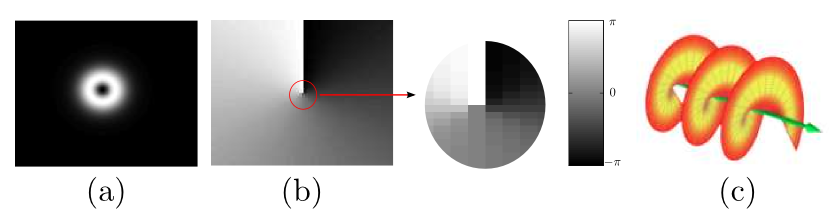
\includegraphics[width=\textwidth,keepaspectratio]{Caps/Imagenes/dibujo.png}
  \caption[Vórtice óptico.]{Vórtice óptico.((a) Perfil de intensidad, (b) fase de variación azimutal $\theta$ y (c) perfil de propagación de la fase).}
  \label{fig:VO}
\end{figure}

Ahora bien, se observa que su distribución de intensidad posee un núcleo con intensidad nula, este hecho es explicable desde una perspectiva de la interferencia destructiva entre los rayos difractados hacía el centro. Consideremos un circulo de radio infinitesimal ubicado en el centro del OV, si al interior del círculo cada punto tiene una fase $\Phi_k$, existe un punto con fase $\Phi_k + \pi$ ubicada de forma simétrica al centro del OV, y de acuerdo al principio de Huygens \cite{Hecht2000} todos los puntos radiarán hacia el centro del círculo, dando lugar a la interferencia destructiva si la diferencia de fase entre dos puntos simétricos es de $\pi$, por consiguiente es de esperar que hayan múltiples puntos donde la intensidad sea nula \cite{Rozas1999,King2010}.\\

Una descripción común para el campo eléctrico de un OV son las bien conocidas funciones Laguerre-Gauss (LG), que son soluciones a las ecuaiones de Maxwell para la radiación en problemas con simetría cilíndrica, y que de forma normalizada están dados por \cite{Uribe2011},
\begin{equation}
\label{eqV2}
	LG_{l,p}(r,\phi) = (\frac{2p!}{\pi (|l|+p)!})^{1/2} \frac{1}{w} (\frac{\sqrt{2}r}{w})^{|l|} L_{p}^{|l|}(\frac{2r^2}{w^2}) \exp (-\frac{r^2}{w^2}) \exp (il\phi),
\end{equation}

donde $(r,\phi)$ representan coordenadas polares, $w$ es el ancho del haz, $l$ y $p$ son los ordenes azimutal y radial respectivamente, que describen la amplitud del campo en términos de $r$ y $L_p^{|l|}$ son los polinomios asociados de Laguerre \cite{SepulvedaSoto2009}, definidos como 

\begin{equation}
\label{eqV3}
\begin{matrix}
	L_p^l(x) = \frac{1}{p!} \frac{d^l}{dx^l} L_p(x)\\
	L_p(x) = \frac{1}{p!} e^x \frac{d^p}{dt^p} (x^p e^{-x})
	 \end{matrix}
\end{equation}


De la Eq.\ref{eqV2} se obtiene la representación de un OV de carga topológica $l$ para cualquier $l \neq 0$ \cite{Uribe2011}, como se muestra en la figura\ref{fig:modsLG}, en donde están algunas funciones Laguerre-Gauss, nótese que la función $LG_{0,0}$ corresponde a una distribución Gaussiana.\\

\begin{figure}[!ht]
  \centering
    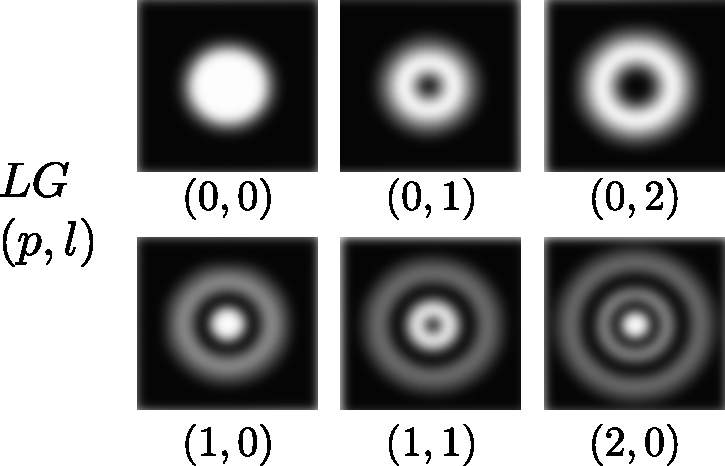
\includegraphics[scale=1]{Caps/Imagenes/LGmodos.pdf}
  \caption{Modos Laguerre-Gauss.}
  \label{fig:modsLG}
\end{figure}


Los OVs pueden ser de dos tipos, los que se mencionaron anteriormente que corresponden a escalares y existe otra clase conocida como OVs vectoriales. Estos últimos son haces generados a partir de patrones de la polarización radial o azimutal, por ejemplo, a través de la superposición de dos haces Hermite-Gauss polarizados ortogonalmente \cite{Cheng2009, Zhan2009}. En la siguiente sección veremos con más detalle algunas de las diferentes maneras de obtener OVs escalares.

\section{Generación de vórtices ópticos}
\label{sec:generacion_vortices}

Una manera de generar OVs es a través de la excitación selectiva de modos Hermite-Gaussianos en láseres \cite{Ohtomo2008}, en donde, a través del control de las propiedades externas e internas de la cavidad de un láser de diodo pueden obtenerse OVs con características específicas de manera \textit{controlada}. Allí el problema es que el control de las propiedades del medio y de la cavidad puede ser un reto experimental complejo. A través de espejos deformables también es posible obtener OVs \cite{Tyson2008}, allí se ajustan las inclinaciones de cada uno de los espejos, de forma tal que se obtiene una superficie esférica con diferentes inclinaciones en sus secciones (produciendo un efecto espiral si se miran de manera general los espejos) y por ende, la diferencia de camino óptico genera una diferencia de fase tal que puede darse una característica helicoidal a la fase. También se han obtenido OVs a través de fibras ópticas \cite{KrishnaInavalli2010, Gao2014}; esto se realiza a través de la manipulación de los estados de polarización de un haz que se propaga por la fibra, y como resultado se tiene una superposición de estados de polarización que produce OVs vectoriales.\\

% , espejos deformables \cite{Tyson2008} y fibras ópticas \cite{KrishnaInavalli2010, Gao2014}
%CGH(Patrón de interferencia producido por un objeto creado computacionalmente) 

%Otras métodos menos comunes son por ejemplo, espejos deformables, en donde se ajustan las inclinaciones de cada uno de los espejos de forma tal que se obtiene una superficie esférica con diferentes inclinaciones en sus secciones, de manera similar a las SPPs, la diferencia de camino óptico genera la diferencia de fase \cite{Tyson2008}. En fibras ópticas, por medio de la manipulación de los estados de polarización pueden obtenerse OVs vectoriales \cite{KrishnaInavalli2010}. Aunque sin duda alguna la forma más común se ha dado con el desarrollo de las pantallas de cristal líquido y de los hologramas generados por computador, en donde, se han generado OVs a partir de moduladores espaciales de luz, en este tema nos centraremos a continuación.


Cuando se modifica la fase directamente, añadiendo en esta una variación azimutal, pueden emplearse diversos elementos, entre ellos, placas de fase espiral \cite{Ruffato2014, Schemmel2014,  Sueda2004} o redes de difracción \cite{Heckenberg1992, Bekshaev2010a, Bekshaev2010}. A continuación describiremos algunos de los elementos más comunes en la generación de OVs.\\

%Una forma de generar OVs es a través de la excitación selectiva de modos Hermite-Gaussianos en láseres \cite{Ohtomo2008}, en donde, a través del control de las propiedades externas e internas de la cavidad de un láser de diodo pueden obtenerse OVs con características específicas de manera \textit{controlada}. En la sección \ref{sec:vortice_optico} se analizó una descripción matemática de los OVs basada en los modos Hermite-Gaussianos, estos son normalmente empleados para describir el funcionamiento de algunos láseres y es de esperar que de este modo puedan obtenerse OVs. El problema es que controlar las propiedades del medio y de la cavidad puede ser un reto experimental. La segunda manera es a través de la imposición de una fase espiral directamente en el haz, la cual puede realizarse de diferentes formas, entre ellas: placas de fase espiral \cite{Ruffato2014, Schemmel2014,  Sueda2004}, espejos deformables \cite{Tyson2008}, elemento ópticos difractivos tales como redes de difracción \cite{Heckenberg1992, Bekshaev2010a} y fibra óptica \cite{KrishnaInavalli2010, Gao2014}. \\

Una placa de fase espiral (SPP: \textit{spiral phase plate}) es un elemento óptico transparente con una superficie en forma de helicoide, cuyo espesor incrementa de manera azimutal y debido a esto, se produce una diferencia de camino óptico y por tanto una diferencia de fase entre distintos puntos del haz \cite{Sueda2004}. La diferencia de fase entre el punto inicial y final determina la carga topológica, de forma tal que la fase varíe linealmente en dirección axial cuando un haz de luz se propaga a través de la SPP. Normalmente son fabricadas para que los saltos de fase sean múltiplos enteros de $2\pi$ y se manufacturan con polímeros \cite{Schemmel2014, Harm2015} o con métodos holográficos \cite{Cheng2013}. La desventaja de las SPPs es que una vez se fabrican no es posible modificar sus propiedades (por ejemplo, carga topológica) y es por ello que los OVs que se generen poseen las mismas características. La Fig. \ref{fig:sppvo} muestra cómo a partir de un plano objeto definido por una amplitud con distribución Gaussiana y un frente de onda plano, puede obtenerse un frente de onda helicoidal mediante la imposición de una SPP en la propagación del haz. La Fig. \ref{fig:sppreal} es un ejemplo de una SPP creada con métodos holográficos.\\

\begin{figure}[!ht]
  \centering
    \includegraphics[scale=0.7] {Caps/Imagenes/SpiralPhasePlateVO.pdf}
  \caption[Generación de OVs a partir de una SPP.]{Generación de OVs a partir de SPP. Imagen adaptada de Ref.[1]}
  \label{fig:sppvo}
\end{figure}

\begin{figure}[!ht]
  \centering
    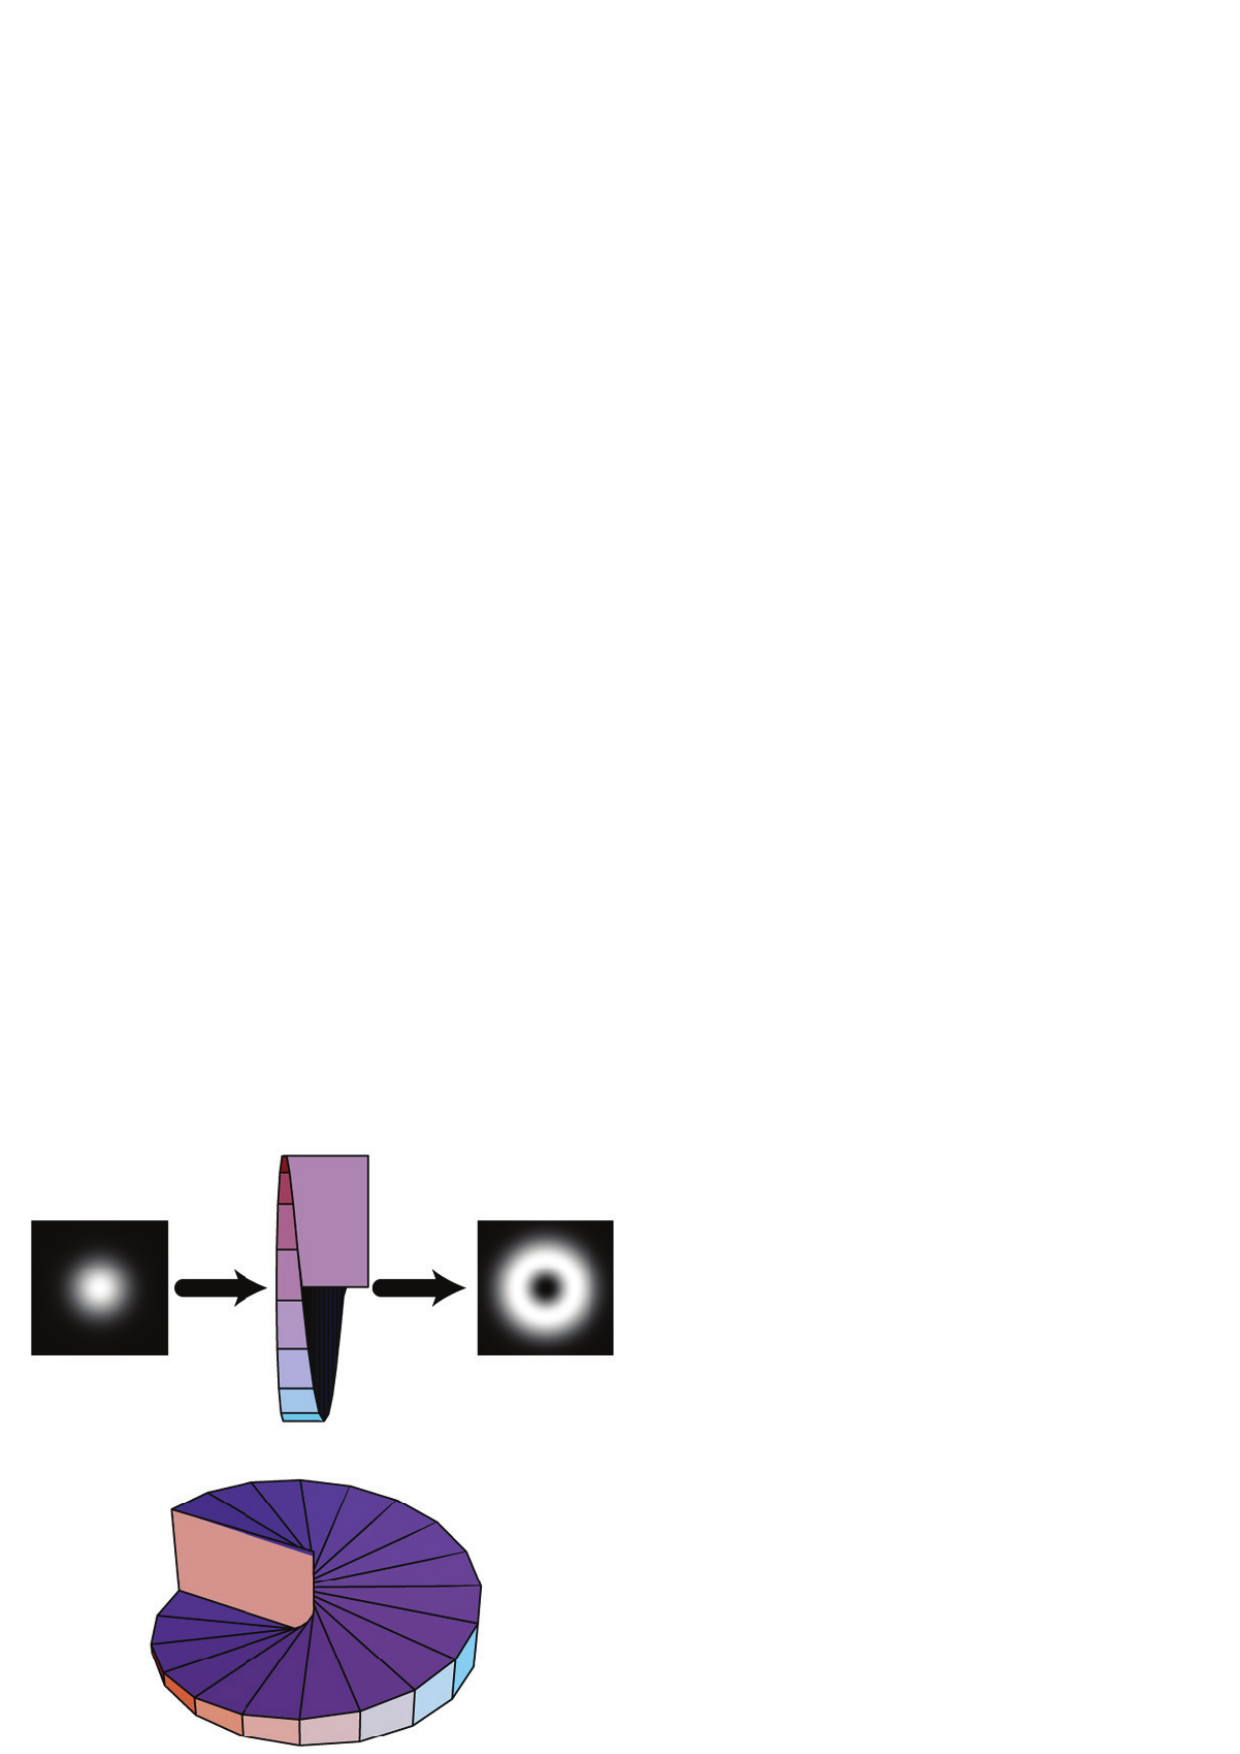
\includegraphics[scale=0.7]{Caps/Imagenes/SPP.png}
  \caption[Placa de fase espiral obtenida por métodos holográficos]{Placa de fase espiral obtenida por métodos holográficos. Imagen adaptada de Ref.[3].}
  \label{fig:sppreal}
\end{figure}

Existe otro método que consiste en la superposición de una red de difracción con una máscara espiral, conocida también como ``redes de difracción bifurcadas'' (\textit{forked grating}) debido a la forma que toma la máscara. El efecto de la adición de una máscara espiral en la red de difracción es la aparición de una transición adicional en la forma de la red, tal como se muestra en la Fig. \ref{fig:forkred}. Los OVs se generan entonces en los ordenes difractados, de forma que si la carga topológica de la máscaras es $q$, el orden $l$ tiene una carga topológica $ql$, es decir, la carga topológica del orden $l = 2$ es $2q$, con $l = 3$ es $3q$ y así sucesivamente \cite{Bazhenov1990, Bekshaev2008, Bekshaev2009}. Una de las mayores ventajas de las redes de difracción es que no necesariamente tienen que ser de fase, se pueden generar OVs empleando redes de amplitud. La Fig. \ref{fig:blazedVO} es un ejemplo de cómo es la distribución de intensidad producido por una red bifurcada del tipo diente de sierra.\\

\begin{figure}[!ht]
  \centering
    \includegraphics[scale=1]{Caps/Imagenes/Gratings.pdf}
  \caption{Obtención de una red de difracción bifurcada.}
  \label{fig:forkred}
\end{figure}

\begin{figure}[!ht]
  \centering
    \includegraphics[scale=0.8]{Caps/Imagenes/DiffGratVO.pdf}
  \caption[Generación de OV a partir de una red de difracción.]{Generación de OV a partir de una red diente de sierra o blazé. Imagen adaptada de Ref.[1].}
  \label{fig:blazedVO}
\end{figure}

Gracias al desarrollo de las pantallas de cristal líquido y de los hologramas generados por computador, la forma más común de generar OVs se ha dado con moduladores espaciales de luz, su funcionamiento será descrito a continuación.

\section{Moduladores espaciales de luz basados en cristal líquido}
\label{sec:slm}

Un modulador espacial de luz (SLM: \textit{spatial light modulator}), es un dispositivo opto-electrónico que como su nombre lo indica, se encarga de modular espacialmente luz y está constituidos por un arreglo de pantallas de cristal líquido (LCDs: \textit{liquid-crystal display}) \cite{Burman2010}. En este contexto \textit{modular} se entiende como variar controladamente las propiedades de la luz, que pueden ser fase o amplitud. Dichos dispositivos emplean la birrefringencia de los cristales líquidos (LCs: \textit{liquid crystal}), de forma tal que mediante un campo eléctrico se rotan los cristales variando así las propiedades de la luz (este concepto se retomará en la sección \ref{subsec:lcdispopt}) \cite{Gennes2007, Cho1998}. Podemos clasificar los SLMs en tres grandes categorías: de fase, de amplitud y aquellos que acoplan ambos efectos. \\

Los SLMs de amplitud son altamente comerciales y permiten variar la intensidad de la luz pixel a pixel en el arreglo de LCDs, es decir, cuando el campo eléctrico es máximo la mayor parte de la luz pasa, cuando es mínimo la luz es absorbida y en los estados intermedios se deja pasar una fracción de la luz, es decir, son de tramitancia variable. Algunos ejemplos de estos son los televisores LCD y los proyectores de vídeo, en estos últimos existe un tipo donde se combinan tres SLMs para generar color con una matriz RGB como se muestra en la Fig. \ref{fig:proyector}.\\

\begin{figure}[!ht]
  \centering
    \includegraphics[width=\textwidth,keepaspectratio]{Caps/Imagenes/Proyector.png}
  \caption[Funcionamiento de un proyector a partir de SLMs.]{Funcionamiento de un proyector a partir de SLMs, variando la intensidad de cada una de las componentes RGB se genera una matriz tal que la imagen generada es a color. Imagen tomada de \small \url{http://www.duiops.net/hifi/cine-en-casa-pantalla-proyectores-lcd.html}}
  \label{fig:proyector}
\end{figure}

Los SLMs de fase son menos comerciales y por lo general más costosos, a diferencia de los SLMs de amplitud, la idea de este tipo de moduladores es que sean capaces de generar una diferencia de fase entre dos puntos cualquiera del arreglo de LCDs y que no generen cambios en la amplitud, la diferencia de fase debe comprender un rango de al menos $[0 - 2\pi]$, de forma que cualquier variación de fase pueda ser representada, dependiendo la longitud de onda. El desarrollo de estos dispositivos ha propiciado el crecimiento de diversas áreas, entre ellas, holografía digital \cite{Jesacher2008}, donde se emplean como generadores de los objetos a registrar,  y en telecomunicaciones \cite{Ahderom2002} por ejemplo, en donde gracias a que las propiedades de la luz puede modificarse punto a punto, es posible transferir diferente información simultáneamente. La Fig. \ref{fig:slm} muestra un SLM PLUTO-VIS-006-A, el cual es de reflexión y solo de fase. \\

\begin{figure}[!ht]
  \centering
    \includegraphics[scale=0.5]{Caps/Imagenes/SLM.jpg}
  \caption{Modulador espacial de luz HOLOEYE-Pluto.}
  \label{fig:slm}
\end{figure}

%Ahora bien, debido a las características de los SLM, la modulación de fase o amplitud se ve influida por el estado de polarización tanto de entrada como de salida de la luz \cite{Iemmi2001, Moreno2003} y por tanto si se desea una modulación solamente de fase, es necesario caracterizar los estados de polarización ante los cuales esta es máxima. Para este proyecto nos centraremos en el HOLOEYE-LC2002\footnote{\url{http://holoeye.com/spatial-light-modulators/discontinued-devices/}}, que es un SLM de transmisión del tipo nemático trenzado (este concepto se abordará en la sección \ref{subsec:lcdispopt}) y una de sus características es que modula tanto fase como amplitud de manera acoplada, por tanto requiere de una calibración que permita una modulación cercana\footnote{Si se cubre el rango [0 - $2\pi$] es posible representar cualquier valor de fase.} a los $2\pi$y no hayan variaciones considerables en la intensidad. La calibración de un SLM de transmisión puede realizarse a través de un sistema generador-analizador de estados de polarización, de forma que ante diferentes estados de entrada y salida hay mayor modulación de fase o de amplitud, este aspecto se profundizará en el capítulo \ref{cap:implementacion}.

Ahora bien, debido a las características de los SLM, la modulación de fase o amplitud se ve influida por el estado de polarización tanto de entrada como de salida de la luz \cite{Iemmi2001, Moreno2003} y por tanto si se desea una modulación solamente de fase, es necesario caracterizar los estados de polarización ante los cuales esta es máxima. Para este trabajo nos centraremos en el HOLOEYE-LC2002\footnote{\url{http://holoeye.com/spatial-light-modulators/discontinued-devices/}}, que es un SLM de transmisión y una de sus características es que modula fase y amplitud de manera acoplada, por tanto requiere de una calibración que permita una modulación cercana\footnote{Si se cubre el rango [0 - $2\pi$] es posible representar cualquier valor de fase.} a los $2\pi$ y no hayan variaciones considerables en la tramitancia. La calibración de un SLM de transmisión puede realizarse a través de un sistema generador-analizador de estados de polarización, de forma que ante diferentes estados de polarización a la entrada y salida del SLM, haya una mayor modulación de fase o de amplitud.%, este aspecto se profundizará en el capítulo \ref{cap:implementacion}.

%Anteriormente se mencionó que los SLMs dependen de 

%La calibración de un SLM de transmisión puede realizarse a través de un sistema generador-analizador de estados de polarización, de forma que ante diferentes estados de entrada y salida hay mayor modulación de fase o de amplitud \cite{Iemmi2001, Moreno2003}, este aspecto se profundizará en el capítulo \ref{cap:implementacion}.

%Finalmente, para aplicaciones relaciones con la generación de OVs se debe contar con una curva de caracterización que no es entregada por el fabricante. Es importante mencionar que los fabricantes de SLMs tales como HOLOEYE\footnote{\url{http://holoeye.com/}} o Hamamatsu Photonics\footnote{\url{http://www.hamamatsu.com/us/en/index.html}} no entregan el producto caracterizado, la calibración debe ser llevada a cabo por quien quiera emplearlo. Esta calibración se realiza acorde al tipo de SLM, para el proyecto nos centraremos en el HOLOEYE-LC2002 \footnote{\url{http://holoeye.com/spatial-light-modulators/discontinued-devices/}}. El LC2002 es un SLM de transmisión del tipo nemático trenzado (este concepto será trabajado en la sección \ref{subsec:lcdispopt}) y una de sus características es que modula tanto fase como amplitud de manera acoplada, por ello, lo que se busca en su calibración es encontrar un estado de funcionamiento tal que la modulación de fase sea cercana a los $2\pi$ y no hayan variaciones considerables en la intensidad. La calibración de un SLM de transmisión puede realizarse a través de un sistema generador-analizador de estados de polarización, de forma que ante diferentes estados de entrada y salida hay mayor modulación de fase o de amplitud \cite{Iemmi2001, Moreno2003}, este aspecto se profundizará en el capítulo \ref{cap:implementacion}.

\subsection{Cristales líquidos como dispositivos ópticos}
\label{subsec:lcdispopt}

Un cristal líquido es un estado intermedio de la materia que lo poseen algunos compuesto químicos, los cuales comparten características típicas de los líquidos y otras características típicas de los estados cristalinos. Por parte de los líquidos poseen la propiedad de moverse libremente en cualquier dirección, aunque, la mayor parte de los líquidos exhiben propiedades físicas (por ejemplo, eléctricas y magnéticas) isotrópicas por naturaleza, los LCs por su lado son anisotrópicos. Normalmente tienen forma cilíndrica o elipsoidal, lo que hace que posean un eje de simetría llamado \textit{eje director}  y les da la propiedad de ser  \textit{orientables}. Su comportamiento se ve alterado por la temperatura, de hecho, cuando se incrementa la temperatura las moléculas se orientan en cualquier dirección, dando lugar a un líquido isotrópico como se muestra en la Fig. \ref{fig:LC}(a), a esta temperatura se le denomina punto de aclarado (\textit{clearing point}). El estado más común de los LCs se conoce como nemático (\textit{nematic}), en este, las moléculas se mueven libremente en cualquier dirección, aunque mantienen sus ejes directores en la misma dirección (Fig. \ref{fig:LC}(b)). Ahora bien, si se disminuye la temperatura, algunos compuestos de LC adquieren un orden espacial y las moléculas se organizan por capas bidimensionales, y el movimiento se limita solo a las capas Fig. \ref{fig:LC}(c) \cite{Uribe2011}.\\

%En condiciones apropiadas las moléculas de LC poseen un orden de orientación tal que los ejes directores se alinean en la misma dirección, conocido como estado nemático (\textit{nematic}), como se muestra en la Fig. \ref{fig:LC}b. En esta fase, las moléculas del cristal pueden moverse pero no pierden su orientación. Si además de tener un comportamiento nemático, las moléculas poseen un orden, es decir, se organizan por capas como se muestra en la Fig. \ref{fig:LC}c se dice que están en estado esméctico (\textit{smectic}) y el movimiento de las moléculas se da solo por capas \cite{Uribe2011}.

\begin{figure}[!ht]
  \centering
    \includegraphics[width=12cm,keepaspectratio]{Caps/Imagenes/LC.pdf}
  \caption[Estados del cristal líquido.]{Estados del cristal líquido. ((a) líquido isotrópico, (b) nemático y (c) esméctico).}
  \label{fig:LC}
\end{figure}

Una consecuencia de la anisotropía de las moléculas, que proviene de la diferencia de la movilidad de los electrones en las dirección longitudinal y transversal al interior del cristal, es poseer distintas propiedades ópticas y eléctricas en diferentes direcciones si consideramos una onda propagándose en dirección paralela o perpendicular al eje director. Este efecto genera dos fenómenos interesantes, la birrefringencia de las moléculas y la orientación bajo la influencia de un campo eléctrico \cite{Uribe2011, Burman2010}. Dada la diferencia entre la movilidad de los electrones al interior del cristal, un campo eléctrico experimenta dos permitividades o constantes dieléctricas distintas, esto se conoce como anisotropía dieléctrica y produce que el desplazamiento eléctrico y el momento dipolar inducido no necesariamente sea paralelo al campo, como consecuencia, los cristales sufren un torque sobre su eje director de forma tal que éste se alinea con la dirección del campo. Una representación de esto puede observarse en la Fig. \ref{fig:torqueLC}, en ausencia de capo eléctrico, la molécula tiene una orientación vertical Fig. \ref{fig:torqueLC}(a), cuando un campo eléctrico representado por las flechas rojas actúa sobre una molécula de LC ésta experimenta un torque (representado por las flechas verdes) causado por la anisotropía Fig. \ref{fig:torqueLC}(b) y la molécula tiende a rotar su eje director en la dirección del campo. Por último si el campo es lo suficientemente intenso, la molécula rota hasta alinearse completamente con la dirección del campo Fig. \ref{fig:torqueLC}(c). \\

\begin{figure}[!ht]
  \centering
    \includegraphics[width=\textwidth,keepaspectratio]{Caps/Imagenes/torqueLC.pdf}
  \caption[Molécula de LC sometida a un campo eléctrico]{Molécula de LC sometida a un campo eléctrico.((a) Torque ejercido a la molécula cuando se aplica un campo eléctrico; (b) con la presencia del campo, la molécula rota para alienar su eje director con la dirección del campo; (c) si el campo es lo suficientemente intenso, el eje director se alinea con la dirección del campo).}
  \label{fig:torqueLC}
\end{figure}

%La forma más común de encontrar los LCs son las LCDs y allí hay una categoría muy común que son los LCDs de  tipo nemático trenzado (TN-LCD: \textit{twisted-nematic liquid-crystal display}).

Una de las configuraciones más comunes para los LCs son las pantallas de cristal líquido (LCD: \textit{liquid-crystal display}). Las LCDs se encuentran en un configuración común conocida como pantallas de cristal líquido \textit{twisted nematic} (TN-LCD: \textit{twisted-nematic liquid-crystal display}). En este, el cristal líquido se encierra entre dos placas de polímero pulido en una dirección específica, llamadas placas de alineación, de forma que el eje director de los cristales se alinea en dirección paralela al sentido del pulido, es decir, hay una prealineación de las moléculas. Las placas son pulidas en direcciones perpendiculares, de forma tal, que las moléculas en contacto con el polímero están en direcciones perpendiculares. Como estamos en el estado nemático, las moléculas de LC tienden a alinear sus ejes directores y a causa de la perpendicularidad entre las moléculas en la superficie del polímero se da un efecto de giro en los ejes directores de las partículas en el interior de la celda, como se muestra en la Fig. \ref{fig:lcd}. Detrás del polímero se ubican dos placas conductoras  transparentes, comúnmente de oxido de indio y estaño (ITO: \textit{indium tin oxide}), de forma que es posible aplicar una diferencia de potencial y por tanto un campo eléctrico a los LCs. En presencia del campo eléctrico, como se mencionó anteriormente, los ejes directores tienden a alinearse con la dirección de este y por tanto hay una rotación de las moléculas. En esta rotación, las propiedades del medio se hacen homogéneas puesto que las moléculas se encuentran alineadas \cite{Uribe2011, Burman2010}. Comúnmente en una celda se ubican dos polarizadores, uno en la entrada y otro en la salida, de forma tal que la rotación de las moléculas permite regular cuánta luz pasa a través de la celda mediante la rotación de los estados de polarización. Pero en los laboratorios, es común que los polarizadores se supriman y que se empleen estados de polarización generados por un sistema generador-analizador para someter la LCD a condiciones de modulación de amplitud o fase de acuerdo a la aplicación.

\begin{figure}[!ht]
  \centering
    \includegraphics[width=\textwidth,keepaspectratio]{Caps/Imagenes/lcdcelda.png}
  \caption[Celda de LCD \textit{twisted nematic}]{Celda de LCD \textit{twisted nematic}. Cuando no hay campo eléctrico, las moléculas de LC rotan su eje director en función de la dirección de las placas de alineación y por tanto la polarización de la luz rota y se transmite por el segundo polarizador. Cuando ese aplica un campo eléctrico, las moléculas se alinean en la dirección del campo, no hay cambio en la polarización de la luz por tanto no hay luz transmitida. Imagen adaptada de Ref. [11].}
  \label{fig:lcd}
\end{figure}

%\section{Consecuencias de por los moduladores espaciales de luz en la generación de vórtices ópticos}
\section{Aberraciones en vórtices ópticos}
\label{sec:genvoslm}


Cuando se se emplean SLMs para obtener haces con vorticidad óptica, actuando estos como generadores de fases espirales, la manera más apropiada de hacerlo es presentar un holograma generado por computadora que contenga información de una máscara de fase espiral (SPM: \textit{spiral phase mask}). El problema de esto es que cuando se quiere generar una máscara cuya carga topológica sea $1$, se requiere de un SLM capaz de generar un cambio de fase de al menos $2\pi$ y que este cambio incremente proporcionalmente con el campo eléctrico aplicado. Consideraremos entonces una modulación ideal, a aquella que además de alcanzar un cambio de fase de $2\pi$, posee una relación lineal entre el cambio de fase y el campo eléctrico aplicado al LC. En el caso del LC-2002 a causa de su modulación acoplada, cuando se tienen modulaciones de fase cercanas a $2\pi$ las variaciones en amplitud son considerables y por esto, es necesario emplear menores modulaciones de fase de forma tal que la variación en intensidad sea despreciable. Emplear una menor modulación de fase para representar la SPM implica un cambio de fase indeseado puesto que la máscara no cumple las condiciones óptimas y por tanto, hay una aberración inducida en los OVs, tal como se muestra en la Fig. \ref{fig:voslm}. Cuando la modulación es ideal y el sistema óptico está limitado por difracción (Fig. \ref{fig:voslm}(a)), se pueden generar SPM con modulaciones de $2\pi$ lineales (Fig. \ref{fig:voslm}(b)) y por tanto se generan OVs ideales (Fig. \ref{fig:voslm}(c)), pero por otro lado, cuando la modulación no es ideal así el sistema óptico siga siendo limitado por difracción(Fig. \ref{fig:voslm}(d)), la SPM tienen un perfil diferente (Fig. \ref{fig:voslm}(e)) y por tanto, es de esperar que el OV generado difiera del ideal (Fig. \ref{fig:voslm}(f)), esta deformación da lugar una aberración inducida por el SLM.\\


%Cuando se se emplean SLMs en la generación de OVs como generador de fases espirales, la manera más apropiada de hacerlo es presentar un holograma generado por computadora que contenga información de una máscara de fase espiral (SPM: \textit{spiral phase mask}). El problema de esto es que cuando se quiere generar una máscara cuya carga topológica sea $1$, se requiere de un SLM capaz de modular al menos $2\pi$ en fase y en condiciones ideales con una curva de modulación lineal. En el caso del LC-2002 a causa de su modulación acoplada, cuando se tienen modulaciones de fase cercanas a $2\pi$ las variaciones en amplitud son considerables y por esto, es necesario emplear menores modulaciones de fase de forma tal que la variación en intensidad sea despreciable. Emplear una menor modulación de fase para representar la SPM implica un cambio de fase indeseado puesto que la máscara no cumple las condiciones óptimas y por tanto, hay una aberración inducida en los OVs, tal como se muestra en la Fig. \ref{fig:voslm}. Cuando la modulación es ideal y el sistema óptico está limitado por difracción (Fig. \ref{fig:voslm}(a)), se pueden generar SPM con modulaciones de $2\pi$ lineales (Fig. \ref{fig:voslm}(b)) y por tanto se generan OVs ideales (Fig. \ref{fig:voslm}(c)), pero por otro lado, cuando la modulación no es ideal así el sistema óptico siga siendo limitado por difracción(Fig. \ref{fig:voslm}(d)), la SPM tienen un perfil diferente (Fig. \ref{fig:voslm}e) y por tanto, es de esperar que el OV generado difiera del ideal (Fig. \ref{fig:voslm}(f)), esta deformación puede considerarse una aberración inducida por el SLM.\\

\begin{figure}[!ht]
  \centering
    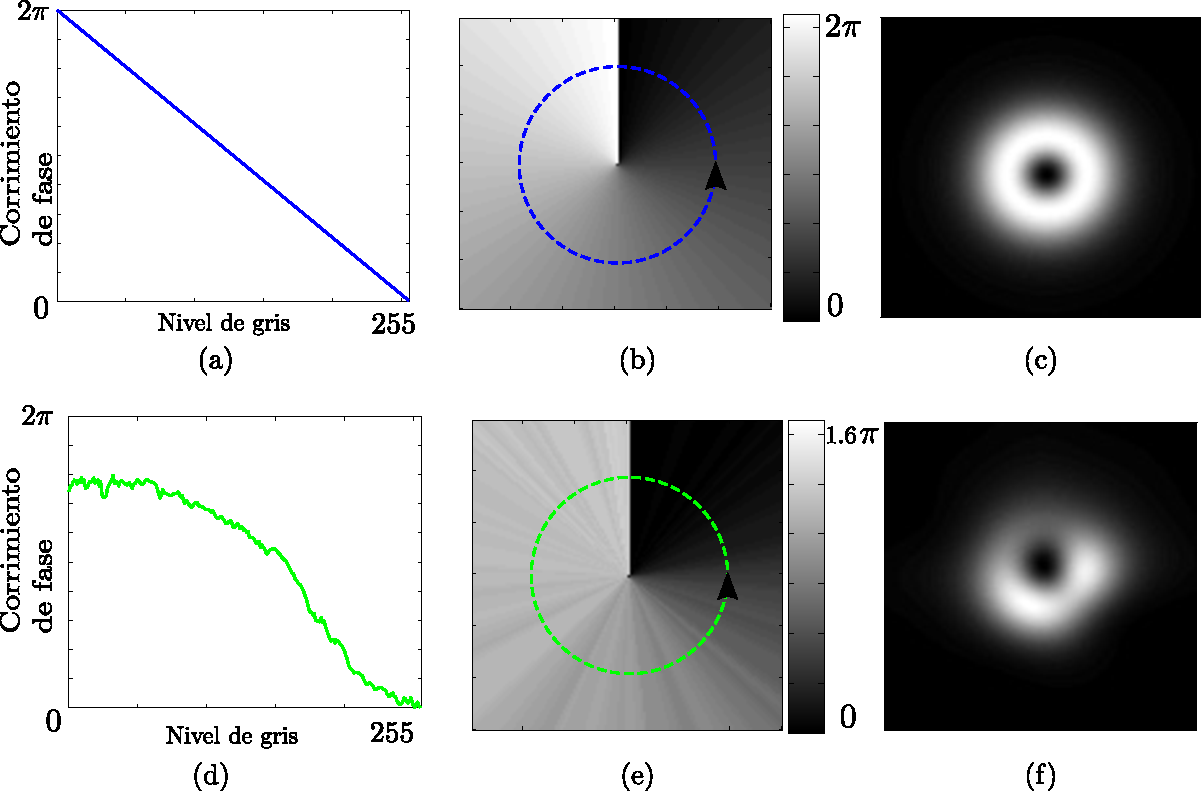
\includegraphics[width=\textwidth,keepaspectratio]{Caps/Imagenes/ovsimreal.pdf}
  \caption[Simulación de OVs ideales y generados con un LC-2002.]{Simulación de vórtices ópticos ideal y generado con un SLM LC-2002. ((a) Curva de modulación ideal, (b) SPM obtenida con una curva de modulación ideal, (c) OV generado de manera ideal, (d) curva de modulación experimental, (e) SPM creada experimentalmente; (f) OV obtenido con la modulación real).}
  \label{fig:voslm}
\end{figure}

Como es bien sabido, cuando un campo se propaga a través de un sistema óptico este es susceptible a aberraciones que pueden ser producidas por los elementos ópticos, las aberraciones se manifiestan como una perdida en la resolución de la imagen recuperada a partir de un objeto\footnote{Este tema será tratado posteriormente en la sección \ref{sec:aberraciones}}. Conocer las aberraciones permite su corrección mediante la manipulación del sistema óptico, por ejemplo, si conocemos que la aberración de nuestro sistema óptico es a causa de un desalineamiento, este podría ser intervenido experimentalmente a través de la realineación del sistema; o mediante la adición de un desfase que contrarreste el aporte de las aberraciones \cite{Liesener2004, Cizmar2011}. Dentro de los métodos más comunes de recuperación de fase existen dos categorías en las cuales tenemos los métodos interferométricos (directos) y los no interferométricos (indirectos). En el caso de los métodos intereferométricos \cite{Creath1988, Malacara2007}, a partir de un patrón de interferencia puede encontrarse la fase de un campo objeto y las aberraciones del sistema, para esto existen diversos métodos y algoritmos, por ejemplo, el método de 4 pasos, en donde a partir de cuatro intensidades cada una con un salto de fase determinado puede recuperarse la fase inicial; esta fase recuperada puede ser descompuesta en términos de polinomios que represantan aberraciones físicas y una vez conocidas pueden ser compensadas. Por otro lado, los métodos no interferométricos se basan en las medidas de intensidad directamente \cite{Soloviev2006, Chanan2000}. Un ejemplo de esto es el sensor Shack-Hartmann, en el cual a partir de un arreglo de microlentes sensa el el frente de onda a través del calculo de la desviación de los centros focales.\\

A través de la determinación de las aberraciones producidas por los elementos sistema óptico en los OVs, pueden también corregirse las aberraciones que estos presentan. En nuestro caso, proponemos implementar un método de recuperación de fase no interferométrico que se conoce como diversidad de fase, este concepto lo trataremos en el siguiente capítulo.

\chapter{Diversidad de fase}
\label{cap:diversidad}

A las técnicas de recuperación de fase no interferométrico pertenece una familia conocida como \textit{Phase Retrieval}; en general, esta familia se basa en algoritmos iterativos para determinar la fase, mediante un problema inverso de múltiples observaciones. El método conocido como diversidad de fase (PD: \textit{phase diversity}) es un tipo de \textit{Phase Retrieval} en donde se añade redundancia al algoritmo de forma que las aberraciones recuperadas son más precisas.\\

%conocido como diversidad de fase (PD: \textit{phase diversity}), el cual  de técnicas de recuperación de fase ; 

%A las técnicas de recuperación de fase no interferométrico pertenece uno conocido como diversidad de fase (PD: \textit{phase diversity}), el cual pertenece a una familia de técnicas de recuperación de fase conocida como \textit{Phase Retrieval}; en general, esta familia se basa en métodos iterativos para determinar la fase.\\

En este capítulo abordaremos el concepto de PD desde su planteamiento inicial para sistemas ópticos con iluminación incoherente y analizaremos el funcionamiento del algoritmo. Analizaremos cómo pueden describirse las aberraciones ópticas a partir de los polinomios de Zernike, y luego plantearemos un nuevo PD para sistemas con iluminación coherente. Posteriormente se propondrán dos modificaciones sobre PD coherente basadas en la curva de modulación en fase del SLM. En la sección \ref{sec:est_arte} se hará una breve introducción sobre PD. A continuación en la sección \ref{sec:div_fase_trad} se abordará el concepto de PD. En la sección \ref{sec:aberraciones} se tratarán las aberraciones ópticas a partir de los polinomios de Zernike; luego en la sección \ref{sec:PD_coherente} se planteará un modelo de PD para sistemas con iluminación coherente, lo cual es una ampliación del Capítulo \ref{cap:vortices}. Finalmente, en la sección \ref{sec:pd12} plantearemos dos modificaciones sobre PD coherente que permitirán diferenciar las aberraciones que son ocasionadas por la modulación de un SLM con las del sistema óptico.

%Dado que el método implementado para la detección de las aberraciones presentes en vórtices ópticos surge de una técnica empleada en sistemas con iluminación incoherente conocida como diversidad de fase (PD: \textit{phase diversity}), en este capítulo analizaremos a fondo la propuesta tradicional de PD y las modificaciones realizadas sobre este, a fin de obtener no solo un PD coherente, si no que a partir de este generar dos conceptos de corrección adicionales basados en información adicional del SLM. Con estos nuevos conceptos se pretende poder distinguir la contribución a las aberraciones del sistema óptico y del SLM. A continuación, la sección \ref{sec:est_arte} es una revisión histórica del desarrollo de PD. En la sección \ref{sec:div_fase_trad} se presentará el postulado inicial de PD, es decir, desde la reconstrucción en sistemas con iluminación incoherente. En la sección \ref{sec:aberraciones} veremos por qué es posible expresar un frente de onda en términos de una serie de los bien conocidos polinomios de Zernike y cómo se puede aplicar esto a PD. Luego, retomaremos PD para proponer su aplicación a sistemas con iluminación coherente y en específico a OVs en la sección \ref{sec:PD_coherente}. Finalmente, veremos cómo a partir de información adicional del SLM y de PD coherente podemos plantear un modelo de determinación de aberraciones causadas por sistemas ópticos y por SLMs.

%Diversidad de fase (PD: \textit{phase diversity}) es un método no interferométrico de sensado de fase que pertenece a una familia de métodos de recuperación de fase conocida como \textit{Phase Retrieval}, en general, esta familia se basa en la determinación de la fase de una manera iterativa.\\

%En este capítulo abordaremos el concepto de PD desde su planteamiento inicial para sistemas ópticos con iluminación incoherente y analizaremos cómo funciona en este caso el algoritmo. Analizaremos cómo pueden describirse las aberraciones ópticas a partir de los polinomios de Zernike, y luego plantear un nuevo PD para sistemas con iluminación coherente y posteriormente se propondrán dos modificaciones sobre PD coherente. En la sección \ref{sec:est_arte} se hará una breve introducción sobre PD. A continuación en la sección \ref{sec:div_fase_trad} se abordará el concepto de PD. En la sección \ref{sec:aberraciones} se tratarán las aberraciones ópticas a partir de los polinomios de Zernike, luego en la sección \ref{sec:PD_coherente} se planteará un modelo de PD para sistemas con iluminación coherente, lo cual es una ampliación del Capítulo \ref{cap:vortices}. Finalmente, en la sección \ref{sec:pd12} plantearemos dos modificaciones sobre PD coherente que permitirán diferenciar las aberraciones que son ocasionadas por la modulación de un SLM con las del sistema óptico.


\section{Introducción}
\label{sec:est_arte}

%(PD: \textit{Phase diversity})

El método de PD fue planteado en 1982 por Gonsalves \cite{Gonsalves1982}, quien propone un sensor de frente de onda (WFS: \textit{Wave-front sensor}) basado en la captura de dos imágenes simultáneas de una misma fuente, en donde una de las imágenes se encuentra en un plano focal, mientras que la otra se encuentra desenfocada una cantidad conocida. A la imagen adicional que se encuentra desenfocada, se le conoce como \textit{diversidad de fase}. En este caso, Gonsalves parametriza la fase en términos de los polinomios de Zernike y demuestra por medio de simulaciones, que a través de un algoritmo iterativo puede obtenerse una estimación de las aberraciones del sistema óptico. \\

En 1988 Paxman et al \cite{Paxman1988} emplean la técnica planteada por  Gonsalves para sensar desalineamientos en telescopios de múltiples espejos deformables. Allí, además de corregir el desalineamiento, logran compensar las aberraciones que se introducen debido a la turbulencia atmosférica, resultado simulado anteriormente por Gonsalves. Pero es en 1992 cuando Paxman et al \cite{Paxman1992} proponen emplear PD como sensor de aberraciones para sistemas ópticos con iluminación incoherente, considerando un número arbitrario de diversidades de fase.% Desde entonces PD ha sido empleado en diferentes problemas que involucran óptica adaptativa \cite{Lofdahl1994, Korkiakoski2012, Sauvage2007, Schgallis2007} o como WFS \cite{Bonet2005, Sauvage2012, Lofdahl1998}, por ejemplo, Lofdahl1994 et al \cite{Lofdahl1994} lo emplean para la corrección de frentes de onda mediante el control de espejos de espejos deformables.

%Pero es en 1992 cuando Paxman et al \cite{Paxman1992} proponen emplear PD como sensor de aberraciones para sistemas ópticos con iluminación incoherente, considerando un número arbitrario de diversidades de fase. Desde entonces PD ha sido empleado en diferentes problemas que involucran óptica adaptativa, observación solar o WFSs \cite{Lofdahl1994, Bonet2005, Korkiakoski2012, Sauvage2007, Sauvage2012, Lofdahl1998, Schgallis2007}.

\section{Diversidad de fase incoherente}
\label{sec:div_fase_trad}

%Como se mencionó anteriormente, PD es un método de sensado de frente de onda para sistemas ópticos con iluminación incoherente, que al igual que otros métodos no interferométricos se basa en medidas de intensidad del campo que se propaga por un sistema óptico. En este se emplean dos imágenes, una que proviene de un plano focal y otra que proviene de un plano desenfocado una distancia conocida $d$, como se muestra en la Fig. \ref{fig:pd}. 
%Este método es no interferométrico y por la, cuando se recupera solo la aberración del sistema óptico corresponde a PD, pero cuando se hace una estimación del objeto y la fase se refiere a PR.\\

Como se mencionó anteriormente, PD es un método de sensado de frente de onda que pertenece a una categoría de WFSs no interferométricos conocidos como \textit{Phase Retrieval}, estos se basan en medidas de intensidad para recuperar de manera iterativa las aberraciones causadas por un sistema óptico empleando o bien esquemas de propagación o algoritmos de búsqueda de gradiente (GSAs: \textit{gradient search algorithm}). PD está planteado para ser un algoritmo de tipo GSA, de modo que a través de un problema inverso de múltiples observaciones se recupera la fase. En su planteamiento inicial se emplean dos imágenes, una que proviene de un plano focal y otra que proviene de un plano desenfocado una distancia conocida $d$, como se muestra en la Fig. \ref{fig:pd}. \\


\begin{figure}[!ht]
  \centering
    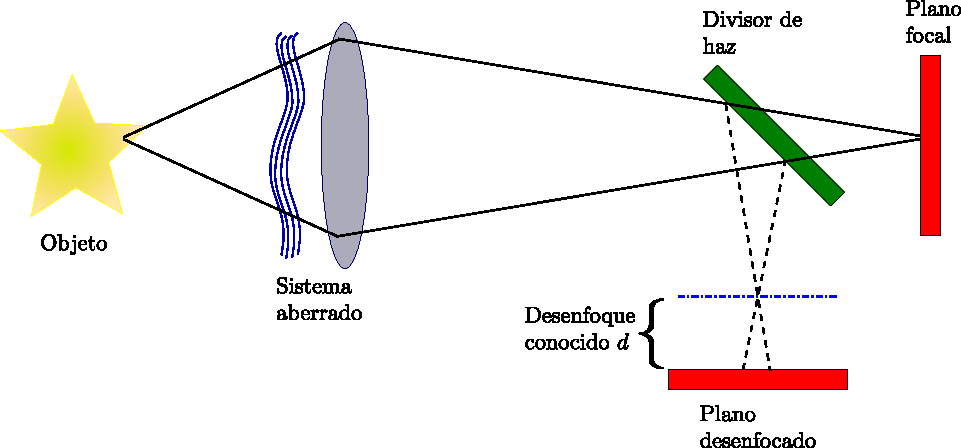
\includegraphics[width=\textwidth,keepaspectratio]{Caps/Imagenes/pd.pdf}
  \caption{Esquema de PD incoherente.}
  \label{fig:pd}
\end{figure}

Consideremos un objeto que es iluminado con luz espacialmente incoherente, si el sistema es lineal\footnote{Recordemos que los sistemas ópticos con iluminación incoherente son lineales con respecto al módulo cuadrado de la amplitud compleja, es decir, con respecto a la intensidad.} e invariante ante el desplazamiento, el plano imagen $d(\vec{x})$ que produce dicho objeto es,

\begin{equation}
\label{eqD1}
	d(\vec{x})= d_{obj}(\vec{x}) \otimes s(\vec{x}),
\end{equation}

donde $\vec{x}$ es un vector de posición bidimensional de coordenadas $(x,y)$, $s(\vec{x})$ la función de punto extendido (PSF: \textit{point-spread function}), $d_{obj}(\vec{x})$ es la irradiancia ideal de la imagen obtenida desde la óptica geométrica \cite{Goodman2005} y $\otimes$ representa la función convolución definida como,
%%% 
%d_obj esta definida como desde el plano imagen se vería el objeto usando la óptica geométrica sin aberraciones
%%%
\begin{equation}
\label{eqD1a}
\begin{aligned}
	d_{obj}(x,y) \otimes s(x,y) & = \mathscr{F}^{-1}\{ \mathscr{F}\{d_{obj}(x,y)\} \mathscr{F} \{s(x,y)\}\}\\
	& = \iint\limits_{-\infty}^{\infty} d_{obj}(\xi,\eta) s(x-\xi,y-\eta) d\xi d\eta
\end{aligned}
\end{equation}

De acuerdo al teorema de la convolución podemos expresar la Eq. \ref{eqD1} en función de sus transformadas de Fourier (FTs: \textit{Fourier transforms}),

%donde $\vec{x}$ es un vector de posición, $d_{obj}(\vec{x})$ el plano objeto, $s(\vec{x})$ la función de punto extendido (PSF: \textit{point-spread function}) y $\otimes$ representa la función convolución definida como. De acuerdo al teorema de la convolución podemos expresar la Eq. \ref{eqD1} en función de sus transformadas de Fourier así

\begin{equation}
\label{eqD2}
	D(\vec{u}) = D_{obj}(\vec{u}) S(\vec{u}),
\end{equation}

donde $\vec{u}$ es un vector de frecuencias espaciales bidimensionales definido en términos de $(\xi , \eta)$, $D(\vec{u}) = \mathscr{F}\{d(\vec{x})\}$, $D_{obj}(\vec{u}) = \mathscr{F} \{d_{obj}(\vec{x})\}$ y $S(\vec{u})=\mathscr{F} \{s(\vec{x})\}$. Para un sistemas con iluminación incoherente $S(\vec{u})$ es la función de transferencia óptica (OTF: \textit{optical transfer function}) \cite{Goodman2005} y puede definirse como,

\begin{equation}
\label{eqD3}
	S(\vec{u}) = H(\vec{u}) \star H(\vec{u}),
\end{equation}

que es la autocorrelación de la función de transferencia coherente $H(\vec{u})$ (CTF: \textit{coherent transfer function}) dada por,

\begin{equation}
\begin{aligned}
	H(\xi,\eta) \star H(\xi,\eta) &= H(\xi,\eta) \otimes H^{\ast}(-\xi,-\eta) 
	\\&= \iint\limits_{-\infty}^{\infty} H(p,q) H^{\ast}(p-\xi,q-\eta) dp dq.
	\end{aligned}
\end{equation}

La FT de la función de respuesta al impulso $h(\vec{x})$ corresponde a $H(\vec{u})$, y $h(\vec{x})$ está relacionada con la PSF, dado que $s(\vec{x}) = |h(\vec{x})|^2$, es decir, la función pupila generalizada (GP: \textit{generalized pupil}), y tiene la forma,

%Sabemos que $H(\vec{u})$ es la FT de la función de respuesta al impulso $h(\vec{x})$ y que $h(\vec{x})$ está relacionada con la PSF, ya que $|h(\vec{x})|^2$ es la PSF, es decir, la función pupila generalizada (GP: \textit{generalized pupil}) y tiene la forma,

%A su vez, la CTF en la Eq. \ref{eqD3} tiene la forma

\begin{equation}
\label{eqD4}
	H(\vec{u}) = \mathscr{F}\{h(\vec{x})\} = A(\vec{u}) \exp\{i \phi(\vec{u})\},
\end{equation}

con $A(\vec{u})$ definida como la tramitancia de la pupila y $\phi(\vec{u})$ la fase introducida por la pupila en el plano de Fourier si estamos en un sistema $4f$, como es nuestro caso.\\ %es decir, $H(\vec{u})$ puede interpretarse como la función pupila generalizada. Como es bien sabido, a través de función pupila generalizada se pueden describir las contribuciones de fase introducidas por el sistema óptico en un plano de Fourier así como la forma y tramitancia de la apertura.

Si modificamos la GP, por ejemplo, añadiendo una diversidad de fase conocida de forma $\Delta H_1 = \exp(\Delta \phi_1 (\vec{u}))$, tenemos una nueva GP $H_1(\vec{u})$ tal que,

\begin{equation}
\label{eqD4a}
\begin{aligned}
	H_1(\vec{u}) & = A(\vec{u}) \exp\{i [ \phi(\vec{u}) + \Delta \phi_1(\vec{u})] \}\\
	& = H(\vec{u}) \Delta H_1(\vec{u}).
\end{aligned}
\end{equation}

De forma que si tomamos la autocorrelación de esta nueva GP ($S_1(\vec{u})$), produciremos una versión distorsionada $D_1(\vec{u})$ de la imagen inicial $D(\vec{u})$, dado que,

\begin{equation}
	D_1(\vec{u}) = D_{obj}(\vec{u}) H_1(\vec{u}),
\end{equation}

la diferencia entre $D(\vec{u})$ y $D_1(\vec{u})$ está dada justamente por la diversidad de fase que hemos añadido. Si podemos agregar un conjunto de $j$ diversidades de fase a la GP, entonces produciremos $D_{j}(\vec{u})$ imágenes distorsionadas, con $j=1,2,...,k$, de $D(\vec{u})$, y para estas tenemos que,


%por tanto la diferencia entre $G(\vec{u})$ y $G_1(\vec{u})$ es la diversidad de fase que hemos añadido. En PD se encuentran las aberraciones a través de la búsqueda de una distribución de fase $\phi (\vec{u})$ que junto con la tramitancia de la pupila $A (\vec{u})$ recupere la OTF que produce no solo la imagen inicial $G(\vec{u})$, si no que además produce la imagen distorsionada $G_{1}(\vec{u})$. Si podemos agregar un conjunto de $k$ diversidades de fase a la pupila generalizada, entonces produciremos $G_{1...k}(\vec{u})$ imágenes distorsionadas de $G(\vec{u})$ y para estas se tiene que,

%El objetivo de encontrar las aberraciones de fase en PD consiste en buscar una distribución de fase $\phi (\vec{u})$ que junto con la tramitancia de la pupila $A (\vec{u})$ recupere la OTF que produce no solo la imagen inicial $G(\vec{u})$, si no que además produce la imagen distorsionada $G_{1}$. Si podemos agregar $k$ diversidades de fase a la pupila generalizada, entonces produciremos $G_{1...k}$ imágenes distorsionadas y para estas se tiene que,

%Ahora de acuerdo al concepto de PD hay un conjunto de $k$ imágenes (que pueden ser dos o más) en las cuales el objeto se mantiene constante y hay una diversidad de fase, a partir de las expresiones \ref{eqD2} - \ref{eqD4a} para las $k$ imágenes se tiene que

\begin{equation}
\label{eqD7}
	D_j(\vec{u}) = D_{obj}(\vec{u}) S_j (\vec{u}),
\end{equation}

donde,

\begin{equation}
\label{eqD6}
	S_j(\vec{u}) = H_j(\vec{u}) \star H_j(\vec{u}),
\end{equation}

\begin{equation}
\label{eqD5}
	H_j(\vec{u}) = H(\vec{u})\Delta H_j(\vec{u}).
\end{equation}

%(diferencia que está dada o bien por la variación de fase conocida o por superposición de la variación de fase conocida con las aberraciones que agregue el sistema). \\

Esto quiere decir que cada una de las $j$ diversidades si bien poseen la misma información del objeto, su función de transferencia puede ser diferente puesto que hemos añadido una fase adicional conocida. El objetivo de PD es entonces, encontrar una distribución de fase $\phi (\vec{u})$ que junto con la tramitancia de la pupila $A (\vec{u})$ recupere la OTF que produce no solo la imagen inicial $D(\vec{u})$, sino que además produce las imágenes distorsionadas $D_{j}(\vec{u})$.\\

De la Eq. \ref{eqD7} podemos ver que

\begin{equation}
\label{eqD8}
	D_j(\vec{u}) - D_{obj}(\vec{u}) S_j(\vec{u}) = 0,
\end{equation}

es decir, la Eq. \ref{eqD8} es una medida del error entre la imagen obtenida $D_j(\vec{u})$ y la producida idealmente desde la óptica geométrica $D_{obj}(\vec{u})$ modulada por la PSF. Aquellas implementaciones que se basan en GSA \cite{Paxman1992, Echeverri2015} emplean métodos de búsqueda de gradiente, para optimizar funcionales de la forma,

\begin{equation}
\label{eqD8a}
L(\overline{D}_{obj}, \phi) = \sum\limits_{j=0}^K \sum\limits_{m,n}^{M,N} |D_j(m,n) - \overline{D}_{obj}(m,n) S_j(m,n,\phi)|^2,
\end{equation}

donde $\overline{D}_{obj}$ es la FT del objeto recuperado por el sistema óptico hasta la frecuencia de corte y $D_j$ es la FT de la intensidad medida en cada pixel $(m,n)$ luego de añadir una diversidad de fase conocida $j$. En la práctica el objeto real $D_{obj}$ es desconocido y el funcional de la Eq. \ref{eqD8a} se puede expresar en términos de la fase $\phi$ exclusivamente \cite{Paxman1992, Gonsalves1982}.\\


%Emplear optimización no lineal permiten estimar el objeto y las aberraciones de manera conjunta
%Si tomamos el error cuadrático medio para cada punto en la medida brindada por Eq. \ref{eqD8}, tenemos que el error $E$ es,

%\begin{equation}
%\label{eqD9}
%	E = \sum\limits_{j=0}^{K} \sum\limits_{u,v}^{M,N} |G_j(\vec{u}) - D_{obj}(\vec{u}) S_j(\vec{u})|^2,
%\end{equation}
%
%
%
%donde $D_{obj}(\vec{u})$ es la transformada de Fourier del objeto restaurado por el sistema óptico y $G_{k}(\vec{u})$ es la transformada de Fourier de la intensidad medida luego de agregar una aberración conocida de índice $k$, y el error es entonces, la diferencia para cada punto $\vec{u}$ entre el objeto y la imagen para cada diversidad $k$. Eventualmente Eq. \ref{eqD9} es una estimación de la diferencia punto a punto ($\Sigma_u$) de la transformada de Fourier de la imagen obtenida y la transformada de Fourier del objeto restaurado para cada una de las diversidades de fase ($\Sigma_j$). El objetivo es entonces a través de un método iterativo basado en búsqueda del gradiente (GSA: \textit{gradient search algorithm}) encontrar una PSF tal que el error $E$ sea un valor mínimo, de manera que la fase $\phi (\vec{u})$ obtenida sea la que corresponde a la fase inducida por el sistema óptico.

%al aplicar una corrección sobre la pupila del sistema puedan corregirse las aberraciones.\\


%Esta corrección normalmente se hace de manera computacional, de forma que a través de posprocesamiento se pueda recuperar la información del objeto. Ahora bien, de $H_j(\vec{u})$ es fácil obtener la amplitud de la función pupila generalizada, que normalmente es una máscara binaria constante y el problema se reduce a encontrar una fase $\phi_j(\vec{u})$ que es la información de las aberraciones presentes durante la propagación. Esto es lo que se busca con el algoritmo de PD, aunque si no se conoce el objeto \textit{a priori}, la estimación también debe hacerse sobre este \cite{Paxman1992}.\\

%Debido a que nuestro objetivo es encontrar un conjunto de aberraciones parametrizadas que describan la fase de un sistema formador de imagen, basado en la siguiente sección trataremos las aberraciones ópticas.\\
Puesto que uno de nuestros objetivos es poder recuperar aberraciones en un sistema formador de imagen, en la siguiente sección trataremos las aberraciones ópticas

\section{Aberraciones ópticas}
\label{sec:aberraciones}

Las aberraciones pueden ser entendidas como la diferencia de camino acumulado por una superficie Gaussiana de referencia \cite{Goodman2005} (frente de onda esférico perfecto producido por la pupila de salida del sistema y que converge hacia un punto imagen ideal) y el frente de onda real, como se muestra en la Fig. \ref{fig:wf}. Normalmente han sido descritas en términos de los polinomios de Zernike, que son una base ortogonal y completa. Además, han sido aceptados por la Socidad de Óptica (OSA: \textit{Optical Solciety}) como medio de descripción de aberraciones ópticas en sistemas formadores de imagen, aunque no es la única base en la que puedan ser descritas \cite{Schmidt2010, Dai2008}.\\

%Las aberraciones pueden ser entendidas como la diferencia de camino acumulado por una superficie Gaussiana de referencia \cite{Goodman2005} (frente de onda esférico perfecto producido por la pupila de salida del sistema y que converge hacia un punto imagen ideal) y el frente de onda real, como se muestra en la Fig. \ref{fig:wf}. Normalmente han sido descritas en términos de los polinomios de Zernike, que son una base ortogonal y completa. Además, han sido aceptados por la Socidad Americana de Óptica (OSA: \textit{Optical Solciety of America}) como medio de descripción de aberraciones ópticas en sistemas formadores de imagen, aunque no es la única base en la que puedan ser descritas \cite{Schmidt2010, Dai2008}.

\begin{figure}[!ht]
  \centering
    \includegraphics[scale=1]{Caps/Imagenes/wf.pdf}
  \caption[Función aberración definida a partir de una esfera Gaussiana ideal.]{Función aberración definida a partir de una esfera Gaussiana ideal, $W(x,y)$ corresponde al frente de onda aberrado.}
  \label{fig:wf}
\end{figure}

Los polinomios de Zernike están definidos como \cite{Schmidt2010},

\begin{equation}
\label{eqD10}
	Z^{m}_{n}(r,\theta) = \sqrt{2(n+1)}R^{m}_{n}(r)G^{m}(\theta),
\end{equation}

donde $(r,\theta)$ denota coordenadas esféricas, $n$ y $m$ son índices de variación radial y frecuencia azimutal respectivamente, $R(r)$ es una función radial y $G(\theta)$ es una función azimutal. Existe otra forma de escribir los coeficiente $n$ y $m$ bajo un índice único $i$, dado por,

\begin{equation}
\label{eqD11}
	i = \frac{n^2+2n+m}{2},
\end{equation}

de manera que Eq. \ref{eqD10} adquiere la forma,

\begin{equation}
	Z_i (r,\theta) = \left\{
	\begin{array}{l l}
		\sqrt{2(n+1)}R^{m}_{n}(r)G^{m}(\theta) & \quad \text{si $m\neq 0$} \\
		R^{0}_n(r) & \quad \text{si $m = 0$}
	\end{array} \right.
\end{equation}

Las funciones $R(r)$ y $G(\theta)$ están dadas por,

\begin{equation}
\label{eqD12}
	R^m_n(r) = \sum^{(n-m)/2}_{k=0} \frac{(-1)^k(n-k)!r^{n-2k}}{k!(\frac{n+m}{2}-k)!(\frac{m-n}{2}-k)!},
\end{equation}

\begin{equation}
\label{eqD13}
	G^m(\theta) = \left\{
	\begin{array}{l l}
		\cos(m\theta) & \quad \text{si $i$ es par}\\
		\sin(m\theta) & \quad \text{si $i$ es impar}
	\end{array} \right.
\end{equation}

Por último, para que los polinomios de Zernike sean ortogonales, éstos deben estar definidos sobre un círculo unitario \cite{Dai2008}, por tanto,

\begin{equation}
\label{eqD14}
	|r| \leq 1 \quad \forall \quad Z_i(r,\theta).
\end{equation}

\subsection{Ortogonalidad y composición de los polinomios de Zernike}
\label{subsec:ortogonalidad}


Podemos encontrar que los polinomios de Zernike son ortognales desarrollando las expresiones \ref{eqD11} - \ref{eqD14} en la Eq. \ref{eqD10}, de forma que,

\begin{equation}
\label{eqD15}
	\int_{0}^{1} R^{m}_n(\rho) R^m_{n'}(\rho) r dr = \frac{1}{2n+1} \delta_{nn'},
\end{equation}

\begin{equation}
\label{eqD16}
	\int_0^{2\pi}G^m(\theta)G^{m'}(\theta) d\theta= \pi \delta_{mm'},
\end{equation}

\begin{equation}
\label{eqD17}
	\int_0^{2\pi} \int_0^1 Z_n^m (\rho,\theta) Z_{n'}^{m'} (\rho, \theta) rdrd\theta = \pi \delta_{nn'} \delta_{mm'} = \pi \delta_{ii'}
\end{equation}

donde $\rho = r/r_{max}$ es decir, la posición radial normalizada y $\delta_{ii'}$ es el delta de Kronecker que está definido como,

\begin{equation}
\label{eqD18}
	\delta_{ii'} = \left\{
	\begin{array}{l l}
		1 & \quad \text{si} \quad i = i'\\
		0 & \quad \text{si} \quad i \neq i'.
	\end{array} \right.
\end{equation}

Como es bien sabido, dos funciones o vectores son ortogonales si,

\begin{equation}
\label{eqD19}
	\vec{a_{i}} \cdot \vec{a_{i'}} = \delta_{ii'},
\end{equation}

es decir, que dos polinomios $i$ y $i'$ son ortogonales entre si. Ahora, con la condición de ortogonalidad (Eq. \ref{eqD17}), un frente de onda $W(r,\theta)$ puede ser descrito como una serie de Zernike con coeficientes $a_i$ dada por,

\begin{equation}
\label{eqD20}
	W(r,\theta) = \sum\limits_{i=0}^{\infty} a_i Z_i (r,\theta).
\end{equation}

Los coeficientes $a_i$ de la serie pueden ser encontrados a través de la descomposición del frente de onda como sigue,

\begin{equation}
\label{eqD21}
	a_i = \frac{\int_0^{2\pi} \int_0^1 W(r,\theta) Z_i(r,\theta) rdrd\theta}{\int_0^{2\pi} \int_0^1 Z_i^2(r,\theta) rdrd\theta}.
\end{equation}

Considerando la discretización del plano $(r,\theta)$ efectuada por los instrumentos de medición (por ejemplo una cámara de vídeo o por las simulaciones), se puede expresar la Eq. \ref{eqD24} en términos de las componentes discretas $p$ y $q$ \cite{Schmidt2010}, tal que,

\begin{equation}
\label{eqD22}
	a_i = \frac{\sum\limits_p \sum\limits_q W(x_p,y_q) Zi(x_p,y_q)}{\sum\limits_p \sum\limits_q Z_i^2(x_p,y_q)} ,
\end{equation}

donde $p, q$ representan las posiciones de los píxeles, $p$ en la dirección $x$ y $q$ en la dirección $y$, de forma que el tamaño total de la ventana cumpla la condición impuesta por Eq. \ref{eqD14}.\\

Ahora que hemos explicado cómo es el planteamiento tradicional de PD y cómo es que un frente de onda puede describirse en términos de una serie de Zernike, nos centraremos en una de las propuestas iniciales de este trabajo, esto es, aplicar el concepto de PD a OVs. Para ello, comenzaremos con plantear un modelo de PD coherente.

\section{Diversidad de fase coherente}
\label{sec:PD_coherente}

Para un sistema con iluminación coherente, lineal\footnote{Un sistema óptico con iluminación coherente es lineal respecto a la amplitud del campo complejo.} e invariante ante el desplazamiento \cite{Goodman2005}, el campo imagen $u(\vec{x})$ es,

\begin{equation}
\label{eqDtrol}
	u(\vec{x}) = u_{obj}(\vec{x}) \otimes h(\vec{x}),
\end{equation}
%que es una copia escalada del objeto,
%
%\begin{equation}
%	\tilde{f_{g}}(\vec{x}) = \frac{1}{|M_t|} f_{obj}(\frac{\vec{x}}{M_t}),
%\end{equation}
%
%con $M_t$ la magnificación transversal. Si aplicamos el teorema de la convolución en Eq. \ref{eqD23}, tenemos que,

donde $h(\vec{x})$ es la función respuesta al impulso y $u_{obj}(\vec{x})$ es el campo complejo del objeto. Si empleamos el teorema de la convolución en la Eq. \ref{eqDtrol}, tenemos:

\begin{equation}
\label{eqD24}
	U(\vec{u}) = U_{obj}(\vec{u}) H(\vec{u}),
\end{equation}

con $U(\vec{u})$, $U_{obj}(\vec{u})$ y $H(\vec{u})$ las FTs de $u(\vec{x})$, $u_{obj}(\vec{x})$ y $h(\vec{x})$ respectivamente. Como se mencionó en la Sección \ref{sec:div_fase_trad}, $H(\vec{u})$ es la función de transferencia coherente y corresponde a la función pupila generalizada. De manera similar al tratamiento efectuado en la Sección \ref{sec:div_fase_trad} para sistemas incoherentes, teniendo en cuenta las propiedades de los sistemas coherentes, podemos realizar una modificación sobre la PG añadiendo una diversidad de fase conocida de forma $\Delta H_1 = \exp (\Delta \phi_1 (\vec{u}))$ a la PG,

%con $U(\vec{u})$, $U_{obj}(\vec{u})$ y $H(\vec{u})$ las FTs de $u(\vec{x})$, $u_{obj}(\vec{x})$ y $h(\vec{x})$ respectivamente. Como se mencionó en la Sección \ref{sec:div_fase_trad}, $H(\vec{u})$ es la función de transferencia coherente y corresponde a la función pupila generalizada. De manera similar podemos realizar una modificación sobre la PG añadiendo una diversidad de fase conocida de forma $\Delta H_1 = \exp (\Delta \phi_1 (\vec{u}))$ a la PG,

\begin{equation}
\begin{aligned}
	H_1(\vec{u}) & = A(\vec{u}) \exp\{i [ \phi(\vec{u}) + \Delta \phi_1(\vec{u})] \}\\
	& = H(\vec{u}) \Delta H_1(\vec{u}).
\end{aligned}
\end{equation}

Puesto que estamos en un sistema con iluminación coherente, en lugar de tomar la autocorrelación de la función de transferencia de amplitud (OTF), se emplea directamente la PG, en la Eq. \ref{eqD24},

\begin{equation}
\label{eqD24a}
	U(\vec{u}) = U_{obj}(\vec{u}) H_1(\vec{u}).
\end{equation}

es decir, que la diferencia entre $U(\vec{u})$ y $U_1(\vec{u})$ se da por la diversidad de fase conocida que hemos añadido. De igual manera, al emplear un conjunto de $j$ diversidades por analogía con la Eq. \ref{eqD7} se obtendrá,

\begin{equation}
\label{eq1e}
	U_j(\vec{u}) = U_{obj}(\vec{u}) H_j(\vec{u}).
\end{equation}

La idea es emplear un campo $u_{obj}(\vec{x})$ conocido, como lo es un haz Gaussiano, característico de los láseres, definido como,

\begin{equation}
	u_{obj}(\vec{x}) = \exp \left(-\frac{|(\vec{x})|^2}{ w} \right),
\end{equation}

donde $w$ corresponde al ancho de la distribución. A partir de esto, propagamos $u_{obj}(\vec{u})$ hasta su FT $U_{obj} (\vec{u})$ a través de la PG aberrada, de modo que el campo imagen en coordenadas espaciales será,

\begin{equation}
\label{eqD1x}
	u_j(\vec{x}) = \mathscr{F}^{-1}\{U_{obj}(\vec{u})H_j(\vec{u})\}.
\end{equation}

Se ha descrito el campo imagen en coordenadas espaciales puesto que como se verá más adelante nuestro sistema óptico corresponde a un 4F que forma imagen del campo de entrada empleando dos lentes y por tanto el plano imagen está en coordenadas espaciales. Si medimos la imagen producida por nuestro sistema óptico $d_j(\vec{x})$ por medio de un sensor para cada una de las diversidades conocidas, podemos plantear el funcional equivalente al presentado en la Eq. \ref{eqD8a} para un sistema con iluminación coherente \cite{Paxman1992, Echeverri2015} como

\begin{equation}
\label{eqDfunc}
L(\phi) = \sum\limits_{j=0}^{K} \sum\limits_{m,n}^{M,N} |d_j(m,n) - |u_j(m,n,\phi)|^2|^2,
\end{equation}

que es la diferencia que se produce entre la imagen medida por el sensor, con la imagen ideal del campo para cada uno de los píxeles $(m,n)$ cuando se aplica una diversidad conocida $j$, de forma que hay una fase $\phi(\vec{u})$ que al modificar $H(\vec{u})$ es capaz de reproducir la imagen inicial y las imágenes distorsionadas por $\Delta H_j(\vec{u})$. Nótese que se ha tomado el módulo cuadrado de $u_j$ puesto que el sensor registra la intensidad de la amplitud compleja. En este caso, el objetivo del algoritmo de búsqueda de gradiente, es encontrar la fase $\phi(\vec{u})$ que produzca un mínimo en el funcional $L$.\\
%Pero en este caso

%Como se mencionó en la sección \ref{sec:div_fase_trad}, $H(\vec{u})$ es la función de transferencia coherente y corresponde a la función pupila generalizada

%y de manera similar podemos concluir que para $k$ diversidades de fase,

%\begin{equation}
%\label{eqD25}
%	U_j(\vec{u}) = H_j(\vec{u}) F_{g}(\vec{u}).
%\end{equation}


%\begin{equation}
%\label{eqD26}
%	E_{coh} = g_j(\vec{x}) - |u_j(\vec{x})|^2
%\end{equation}

%Si expresamos el campo imagen en términos de coordenadas espaciales a partir de Eq. \ref{eqD25}, se obtiene,

%\begin{equation}
%\label{eqD25}
%	u_j(\vec{x}) = \mathsrc{F}^{-1} \{ H_j(\vec{u}) F_{g}(\vec{u})\}.
%\end{equation}

%Si aplicamos un tratamiento similar a la sección \ref{sec:div_fase_trad} para $k$ diversidades de fase,

%
%\begin{equation}
%\label{eqD23}
%	S(\vec{u}) = H(\vec{u}),
%\end{equation}
%
%es decir que la CTF no es más que la función pupila generalizada \cite{Goodman2005} y por tanto,
%
%\begin{equation}
%\label{eqD24}
%	G(\vec{u}) = |\tilde{D_{obj}}(\vec{u})|^2 H(\vec{u}),
%\end{equation}
%
%donde $\tilde{D_{obj}}(\vec{u})$ es la imagen ideal predicha por la óptica geométrica, que es una copia escalada del objeto,
%
%\begin{equation}
%\label{eqD24a}
%	\tilde{D_{obj}}(\vec{u}) = \frac{1}{|M_t|} D_{obj}(\frac{\vec{u}}{M_t}),
%\end{equation}
%
%con $M_t$ la magnificación transversal. Nótese que la Eq. \ref{eqD24} se ha tomado el módulo cuadrado de $\tilde{D_{obj}}(\vec{u})$ puesto que los sistemas con iluminación coherente son lineales ante la amplitud del campo complejo. Si realizamos un tratamiento similar a sección \ref{sec:div_fase_trad} para las $k$ diversidades de fase, podemos plantear obtenemos así como en la Eq. \ref{eqD9} que la función error coherente $E_{coh}$ es,
%%Como se mencionó, en la Eq.(\ref{eqD4}) sabemos que la tramitancia $A(\vec{u})$ de la función pupila generalizada es normalmente, una máscara binaria que determina cuánta luz colecta el sistema óptico.  
%
%\begin{equation}
%\label{eqD25}
%	E_{coh} = \sum\limits_j \sum\limits_u |G_j(\vec{u}) - |\tilde{D_{obj}}(\vec{u})|^2 H_j(\vec{u})|^2.
%\end{equation}
%
%es decir, que el error se determina como la diferencia para cada punto $\vec{u}$ entre la transformada de Fourier de la intensidad de la imagen ideal del objeto y la transformada de Forurier de la imagen recuperada luego de agregar una diversidad de fase $k$.

%al ser comparada la intensidad del campo imagen obtenido de las simulaciones con la imagen obtenida, se consiga una imagen que aproxime la imagen al objeto. En este punto se dice que hay una PSF que representa los cambios de fase y los cambios de amplitud introducidos por el sistema óptico. Conociendo esto y describiendo la fase en términos de una serie de Zernike truncada en $N$ (Eq. \ref{eqD20}), podemos escribir la PSF como

%Si conocemos las propiedades del campo objeto y podemos  obtener la transformada de Fourier del campo imagen ideal escalado ($\tilde{D_{obj}(\vec{u})}$), el problema se reduce entonces a encontrar una fase $\phi(\vec{u})$ en la CTF que aproxime $\tilde{D_{obj}(\vec{u})}$ a la transformada de Forurier de la imagen recuperada ($G(\vec{u})$). Podemos expresar 

%Conociendo esto y describiendo la fase en términos de una serie de Zernike truncada en $N$ (Eq. \ref{eqD20}), podemos escribir la PSF como

%\begin{equation}
%\label{eqD26}
%	H(\vec{u}) = A(\vec{u}) \exp\{i \sum\limits_{j=0}^{N} a_j Z_j(\vec{u})\}.
%\end{equation} 
%
%Y si reemplazamos Eq. \ref{eqD26} en la función error Eq. \ref{eqD25}, se obtiene que el algoritmo de GSA aproxima el objeto únicamente a través de variaciones en la fase de la PSF y por tanto es la fase que introduce la función pupila generalizada del sistema óptico \footnote{El campo objeto se conoce de las propiedades del haz a la entrada del sistema, por ejemplo, una distribución Gaussiana con un frente de onda plano y la amplitud de la función pupila es conocida puesto que es una máscara binaria que se mantiene constante en todas las imágenes.}, es decir, se quiere encontrar una fase para la función pupila generalizada $H_j(\vec{u})$ tal que la imagen que me produce el objeto conocido son lo más parecido posible ($E_{coh} \rightarrow 0$).\\

%El próximo paso es juntar el concepto de PD coherente con los conceptos discutidos en el capítulo \ref{cap:vortices}. Supongamos  que tenemos un sistema óptico con iluminación coherente que produce OVs con carga topológica $l$. En la sección \ref{sec:vortice_optico} se concluyó que una de las característica de un OV se encuentra en su factor de fase azimutal $\exp(il\theta)$, de Eq. \ref{eqD24} y Eq. \ref{eqV1} tenemos que el plano imagen $g_l(\vec{u})$ es



Hemos deducido el caso de PD para sistemas con iluminación coherente y como nuestra intención es poder recuperar las aberraciones de un sistema óptico a través de PD aplicado a OVs, aplicaremos los conceptos tratados en el Capítulo \ref{cap:vortices} con lo visto hasta el momento. \\

%El próximo paso es juntar el concepto de PD coherente con los conceptos discutidos en el capítulo \ref{cap:vortices}. Supongamos  que tenemos un sistema óptico con iluminación coherente que produce OVs con carga topológica $l$. En la sección \ref{sec:vortice_optico} se concluyó que una de las característica de un OV se encuentra en su factor de fase azimutal $\exp(il\theta)$, de Eq. \ref{eqD24} y Eq. \ref{eqV1} tenemos que el plano imagen $g_l(\vec{u})$ es

Consideremos un un sistema óptico con iluminación coherente que produce OVs con carga topológica $l$. En la sección \ref{sec:vortice_optico} se concluyó que una de las característica de un OV se encuentra en su factor de fase espiral definida por,
\begin{equation}
	\psi_l (\vec{u}) = \exp(il \theta (\vec{u})),
\end{equation} 
si esta fase es añadida a la PG, es de esperar que su campo imagen $u(\vec{x})$ corresponda a un OV, por ende si el campo imagen es medido con una diversidad de fase $j$ y una fase espiral $l$, tenemos que,

\begin{equation}
\label{eqD27}
	u_{j}^l (\vec{x}) = \mathscr{F}^{-1} \{D_{obj}(\vec{u}) H(\vec{u}) \Delta H_j(\vec{u}) \psi_l (\vec{u})\},
\end{equation}
%con
%\begin{equation}
%\label{eqD28}
%	W_l(\vec{u}) = l\theta + \phi(\vec{u}) + \Delta \phi_0 (\vec{u}),
%\end{equation}

es decir, hemos planteado una nueva familia de diversidades de fase causadas por la presencia de la fase espiral $\psi_l$ para el campo imagen. De manera similar a la Eq. \ref{eqDfunc} podemos obtener un nuevo funcional que dependa no solo de las diversidades causada por aberraciones $\Delta \phi_j (\vec{u})$, si no que también considere una diversidad espiral $\psi _l (\vec{u})$, de manera que si medimos la intensidad producida $d_j^{l}$ para una diversidad espiral $l$ y una diversidad de aberración $j$, el funcional toma la forma,

\begin{equation}
\label{eqDfuncCohere}
L (\phi) = \sum\limits_{l=0}^{L} \sum\limits_{j=0}^{K} \sum\limits_{m,n}^{M,N} |d_j^l(m,n) - |u_j^l(m,n,\phi)|^2|^2
\end{equation}

con lo que se ha añadido la información que es aportada por las diversidades espirales. A a este PD que además de emplear diversidades de aberraciones emplea diversidades espirales lo denominaremos en adelante PD coherente \cite{Echeverri2015}. \\
%la función pupila generalizada contiene la información sobre la fase azimutal $\theta$\footnote{Tener en cuenta que la máscara espiral es añadida en el plano de Fourier y por tanto, el OV se obtiene en el plano imagen.} y las aberraciones que puedan provenir del sistema óptico o de cualquier otro factor, de forma que asociamos $\phi(\vec{u})$ con las aberraciones y $\Delta \phi_0 (\vec{u})$ es una diversidad de fase conocida. Ahora, para emplear el concepto de PD en OVs, tenemos que considerar además del conjunto de imágenes $k$ el conjunto de cargas topológicas $l$ y por tanto planteamos nuestra nueva función error como

%\begin{equation}
%\label{eqD29}
%	E = \sum\limits_l \sum\limits_j \sum\limits_u |G_{k,l} (\vec{u}) - D_{obj}(\vec{u}) A(\vec{u}) W_{l,k}(\vec{u})|^2.
%\end{equation}

%Esto es el error punto a punto ($\Sigma_u$) producido en cada una de las $k$ imágenes ($\Sigma_j$) que posee una carga topológica $l$ ($\Sigma_l$). En este caso, lo que debe encontrar el algoritmo de GSA es una fase $\phi (\vec{u})$ que reproduzca las aberraciones que posea cada OV medido y como se vio en la sección \ref{sec:aberraciones}, esta descripción puede darse en términos de una serie de Zernike. Si no conocemos el objeto $d_{obj}(\vec{u})$ el problema  para el algoritmo de GSA pasa a ser una estimación conjunta de la amplitud y la fase, lo que complica los cálculos, por ende, si podemos conocer o bien de manera teórica, experimental o simulada el campo objeto, retomamos al caso deseado de una estimación puramente de la fase introducida por la PSF del sistema óptico. Entonces para PD coherente es necesario contar \textit{a priori} con la información del objetode forma que la comparación en Eq. \ref{eqD29} sea entre un OV ideal y la imagen que produce el sistema óptico \cite{Echeverri2015}. Por último, es importante mencionar que para generar las SPM y las aberraciones es mejor emplear un SLM puesto que a través de CGHs podemos emplear diferentes combinaciones máscaras-aberraciones.\\

%En la Fig. \ref{fig:pdflux} se muestra el diagrama de flujo del algoritmo de PD coherente. Primero se define una apertura del sistema $A(x,y)$, un conjunto de diversidades dado por las cargas topológicas $arg(e^{il\theta})$ y un conjunto de diversidades dado por las aberraciones $\phi_j$. Luego se realizan las medidas de intensidad experimentales para cada una de las diversidades $g_{k,l}$, $(m,n)$ representa cada uno de los píxeles de la imagen obtenida, con ello se genera un conjunto de  imágenes experimentales. A continuación se genera una simulación $u_{k,l}$ en donde se emplean las mismas propiedades de las experimentales, pero en estas se añade a la función pupila generalizada una fase adicional $\phi$ determinada por el GSA. Esta fase es la que añadiría el sistema óptico a los resultados experimentales. Seguidamente se evalúa la función error $E$, como se definió anteriormente, esta consiste en una suma punto a punto $(m,n)$, para cada una de las $k$ imágenes y cada una de las $l$ cargas topológicas. En esta función error, a la simulación $u_{k,l}$ hay que tomarle el módulo cuadrado puesto que la medida experimental corresponde a una intensidad, para su comparación se necesita entonces que ambos correspondan a intensidades. Como PD es un algoritmo iterativo, si el error es menor que un valor de tolerancia $\varepsilon$, quiere decir que la fase adicional $\phi$ describe las aberraciones del sistema, si no, por medio del GSA se propone una nueva fase y se generan un nuevo conjunto de intensidades simuladas y se repite el ciclo. Más información puede encontrarse en el anexo 1.\\

En la Fig. \ref{fig:pdflux} se muestra el diagrama de flujo del algoritmo de PD coherente. Primero se define una apertura del sistema $A(x,y)$, un conjunto de diversidades espirales $\psi_l$ y un conjunto de diversidades de aberraciones $\phi_j$. Luego se realizan las medidas de intensidad experimentales $d_{j}^l$ para cada una de las diversidades, con lo cual se obtiene un conjunto de imágenes experimentales que poseen las aberraciones $\phi$ causadas por el sistema óptico además de las diversidades conocidas $j$ y $l$. A continuación se genera una simulación donde se obtiene el campo complejo para cada una de las diversidades $u_{j}^l$ donde se emplean las mismas propiedades usadas en las medidas experimentales. En cada iteración del algoritmo se propone una fase $\phi$ a partir de la cual se calcula $u_{j}^l$, de forma que mediante esta última, el algoritmo de búsqueda de gradiente determina la fase $\phi$ que se empleará en la próxima iteración de forma que $L$ tienda a cero. Cuando el algoritmo encuentra un valor mínimo de $L$, la última fase $\phi$ propuesta será la que representa las aberraciones del sistema óptico.\\

% de las experimentales, pero en estas se añade a la función pupila generalizada una fase adicional $\phi$ determinada por el GSA. Esta fase es la que añadiría el sistema óptico a los resultados experimentales. Seguidamente se evalúa la función error $E$, como se definió anteriormente, esta consiste en una suma punto a punto $(m,n)$, para cada una de las $k$ imágenes y cada una de las $l$ cargas topológicas. En esta función error, a la simulación $u_{k,l}$ hay que tomarle el módulo cuadrado puesto que la medida experimental corresponde a una intensidad, para su comparación se necesita entonces que ambos correspondan a intensidades. Como PD es un algoritmo iterativo, si el error es menor que un valor de tolerancia $\varepsilon$, quiere decir que la fase adicional $\phi$ describe las aberraciones del sistema, si no, por medio del GSA se propone una nueva fase y se generan un nuevo conjunto de intensidades simuladas y se repite el ciclo. Más información puede encontrarse en el anexo 1.\\


\begin{figure}[!ht]
  \centering
    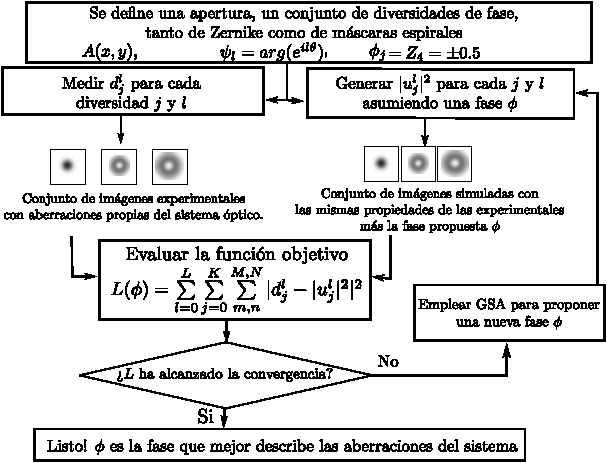
\includegraphics[width=\textwidth,keepaspectratio]{Caps/Imagenes/PDflux.pdf}
  \caption{Diagrama de flujo de PD coherente.}
  \label{fig:pdflux}
\end{figure}

En la Sección \ref{sec:generacion_vortices} se discutió que una de las formas más comunes de generar OVs es a través de SLMs, y cuando se emplean dichos elementos, si su modulación no es cercana a la ideal hay aberraciones inducidas en los OVs. Pero de acuerdo al planteamiento del algoritmo, $\phi$ representa todas las aberraciones del sistema y no es posible identificar de manera directa el aporte a las aberraciones provenientes de la baja modulación en fase del SLM y del sistema óptico, es decir, si bien $\phi$ describe las aberraciones del sistema, no da indicios de la fuente que las genera. Para discernir las aberraciones generadas por la baja modulación del SLM y el sistema óptico, se proponen entonces dos modificaciones sobre PD coherente mediante el empleo de las características reales del SLM.

\section{Modificaciones propuestas para diversidad de fase coherente}
\label{sec:pd12}

Tenemos un algoritmo basado en PD que se encarga de encontrar aberraciones presentes en OVs a partir de la comparación de los resultados experimentales con resultados ideales generados bajo las mismas características. Queremos distinguir las aberraciones causadas por la baja modulación del SLM y por el sistema óptico independientemente; para esto, se propone emplear la curva de modulación del SLM, es decir, analizar los efectos que tiene la modulación de fase real en la generación de OVs a través de simulaciones.\\

%Tenemos un algoritmo basado en PD que se encarga de encontrar aberraciones presentes en OVs a partir de la comparación de los resultados experimentales con resultados ideales generados bajo las mismas características. Queremos distinguir de dónde provienen las aberraciones, para esto, se propone emplear la curva de modulación real (CMR) del SLM, es decir, analizar los efectos que tiene la modulación en la generación de OVs a través de simulaciones

%Puesto que en PD hay una etapa de simulación de OVs, cuando se obtiene $u_j^l$, en esta se asume que la máscara espiral de fase es ideal, pero si tomamos la CMR del SLM entonces se encuentran que los OVs difieren de los ideales. Pensando en emplear la CMR, surge un nuevo simulador de OVs que se basa en los datos de modulación real. De esto nacen dos nuevas posibilidades para hacer PD, las cuales hemos denominado PD1 y PD2 y las trataremos a fondo a continuación. La Fig. \ref{fig:PD012} muestra las tres posibles maneras de generar OVs para PD. La primera de ellas proviene de una simulación ideal de los OVs, de esta se obtiene un conjunto de imágenes completamente ideales. La segunda consiste en la simulación de OVs que poseen una máscara de fase dada por la CMR y por tanto, si bien el sistema óptico es simulado, la modulación es real. La tercera son las imágenes aportadas por el sistema óptico. La pregunta es entonces, ¿qué información se puede obtener de la comparación de cada una de los diferentes generadores de OVs?

Puesto que en PD hay una etapa de simulación de OVs, cuando se obtiene $u_j^l$, en esta se asume que la máscara de fase espiral $\psi_l$ es ideal, de forma que al generar OVs a través de un sistema limitado por difracción, el resultado es un haz toroidal ideal. Pero como fue mostrado en la Sección \ref{sec:genvoslm}, si tomamos la curva de modulación del SLM y simulamos nuevamente la generación de OVs a través de un sistema limitado por difracción, el resultado es una aberración en los OVs a causa de la baja modulación. A partir del empleo de la modulación real del SLM en la simulación de los OVs se proponen dos modificaciones sobre PD coherente, de forma que a través de estas se puedan distinguirse las aberraciones causadas por la baja modulación en fase y las causadas por el sistema óptico. \\

Supongamos que las aberraciones recuperadas por PD coherente corresponden a $\phi_{coh}$, y que estas están compuestas de la aberración a causa de la modulación del SLM $\phi_{slm}$ y las contribuciones del sistema óptico $\phi_{so}$, de forma que,

\begin{equation}
\label{eqPDs}
\phi_{coh} = \phi_{so} + \phi_{slm},
\end{equation}

$\phi_{slm}$ está implícito en la modulación del SLM, entonces si podemos generar OVs que contengan información de la modulación real a través de un sistema limitado por difracción $o_j^l$, tendremos una nueva posibilidad como entrada para el algoritmo de PD coherente, como se muestra en la Fig. \ref{fig:PD012}. Allí se encuentran las tres posibles maneras de obtener OVs que sirven de entrada para PD coherente a partir de la fase que se quiera recuperar. La primera de ellas proviene de una simulación ideal de los OVs  $u_j^l$, en la cual se emplea un sistema limitado por difracción junto con una modulación ideal. La segunda consiste en emplear un sistema limitado por difracción que use la modulación real del SLM $o_j^l$, por tanto estas contienen la fase $\phi_{slm}$ que hace diferir los OVs del caso anterior. La tercera manera son los OVs producidos experimentalmente $d_j^l$.\\
%contienen la información no solo de la modulación del SLM, sino que además la de los elementos ópticos, de forma que podemos separar $\phi_{coh}$ en las contribuciones de la modulación  y del sistema óptico $\phi_{so}$, de forma que la aberración tiene la forma

%\begin{equation}
%\label{eqPDs}
%\phi_{coh} = \phi_{SO} + \phi_{SLM}
%\end{equation}
%si tomamos la CMR del SLM entonces se encuentran que los OVs difieren de los ideales. Pensando en emplear la CMR, surge un nuevo simulador de OVs que se basa en los datos de modulación real. De esto nacen dos nuevas posibilidades para hacer PD, las cuales hemos denominado PD1 y PD2 y las trataremos a fondo a continuación.

%Allí se encuentran las tres posibles maneras de obtener OVs que sirven de entrada para PD coherente a partir de la fase que se quiera recuperar. La primera de ellas proviene de una simulación ideal de los OVs, en la cual se emplea un sistema limitado por difracción junto con una  modulación ideal $u_j^l$, de esto se obtiene un conjunto de OVs ideales. La segunda consiste en emplear un sistema limitado por difracción que emplea la modulación real del SLM $o_j^l$, por tanto estas contienen la fase $\phi_{slm}$ que las hace diferir del caso anterior. La tercera manera son los OVs producidos experimentalmente $d_j^l$.




%La segunda consiste en la simulación de OVs que poseen una máscara de fase dada por la CMR y por tanto, si bien el sistema óptico es simulado, la modulación es real. La tercera son las imágenes aportadas por el sistema óptico. La pregunta es entonces, ¿qué información se puede obtener de la comparación de cada una de los diferentes generadores de OVs?

\begin{figure}[!ht]
  \centering
    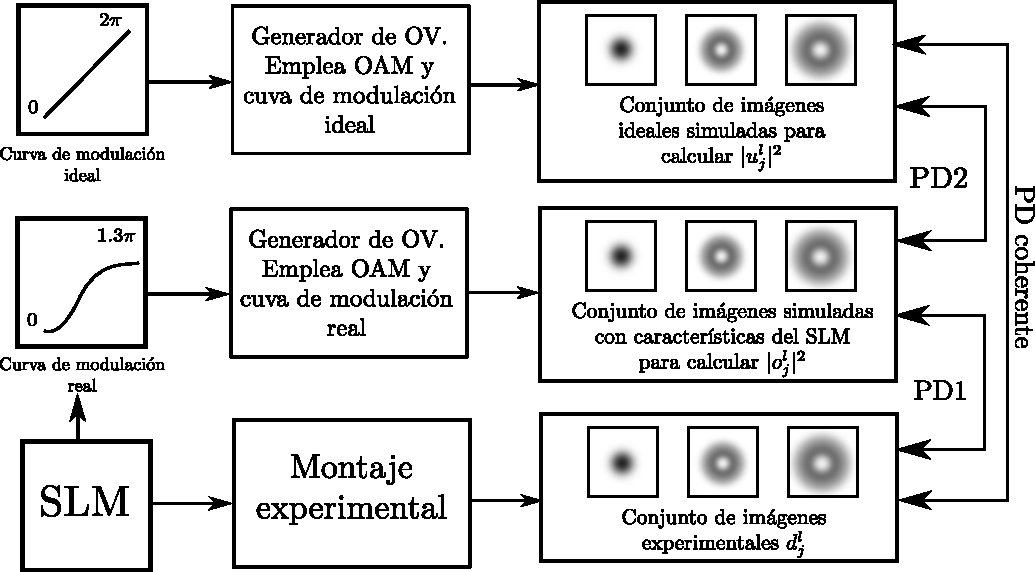
\includegraphics[width=\textwidth,keepaspectratio]{Caps/Imagenes/PD012fulx.pdf}
  \caption{Diagrama de las modificaciones sobre PD coherente.}
  \label{fig:PD012}
\end{figure}

Ahora, si en la Eq. \ref{eqPDs} consideramos que los OVs se producen en un sistema limitado por difracción con una modulación ideal, entonces $\phi_{so} = 0$ y $\phi_{slm} = 0$, por tanto, $\phi_{coh} = 0$, es decir, que si empleamos un sistema y una modulación ideal, no hay aberraciones. Si los OVs se generan con la modulación del SLM estos poseerán $\phi_{slm}$, como es el caso de $o_j^l$ y $d_j^l$, y debido a que ya se ha considerado la aberración por el SLM $\phi_{coh} = \phi_{so}$, y por ende si empleamos  en PD coherente, recuperaremos las aberraciones del sistema óptico $\phi_{so}$ independientes de la modulación del SLM, a esto le llamaremos PD1. Por último, si los OVs se generan por un sistema limitado por difracción y difieren únicamente por la modulación del SLM (empleando $u_{j}^{l}$ y $o_{j}^l$), $\phi_{so} = 0$ y $\phi_{coh} = \phi_{slm}$, a esto lo llamaremos PD2.\\

Como se muestra en la Fig. \ref{fig:PD012} si comparamos un conjunto de OVs generados idealmente con los que se generan desde el montaje experimental, estamos en el caso de PD coherente, es decir, un conjunto global de aberraciones $\phi_{coh}$ que presentan los OVs. Pero si la comparación es entre OVs ideales con aquellos generados por un sistema limitado por difracción con una modulación real (fila 2), la información que obtendremos corresponde a la aberración que introduce la modulación del SLM $\phi_{slm}$ (PD2). Esto es debido a que no estamos tomando resultados experimentales, de hecho, en ambos la propagación por el sistema óptico es simulada y se asume un sistema óptico limitado por difracción, lo que difiere es la característica de la modulación y por ende es de esperar que las aberraciones recuperadas correspondan a las inducidas únicamente por el SLM. Ahora si comparamos los resultados experimentales con los OVs que se generan mediante el sistema óptico limitado por difracción y la modulación del SLM, las aberraciones que se obtienen corresponden a las que son causadas por el sistema óptico $\phi_{so}$ (PD1). Esto es debido a que la aberración causada por la modulación del SLM se encuentra presente en ambos resultados y lo que difiere es el sistema óptico. La información obtenida con cada una de las modificaciones de PD se resume en la Tabla \ref{tab:pd012}.

\begin{center}
\begin{table}
	\centering
	\begin{tabular}{|c|p{8cm}|}
	\hline 
	PD coherente & Aberraciones globales 
	causadas por el SLM y el sistema óptico. \\ 
	\hline 
	PD1 & Aberraciones causadas por la 
	propagación de la luz a través del sistema óptico. \\ 
	\hline 
	PD2 & Aberraciones causadas por la 
	diferencia entre la modulación ideal-real. \\ 
	\hline 
	\end{tabular} 
	\caption{Información de las aberraciones recuperada de las modificaciones sobre PD coherente.}
	\label{tab:pd012}
\end{table}
\end{center}

Podemos definir dos nuevos funcionales similar a la Eq. \ref{eqDfuncCohere} para PD1 y PD2, puesto que solo modificamos las intensidades $|u_{j}^{l}|^2$, $|o_{j}^l|^2$ y $d_{j}^l$ de entrada para PD coherente, de forma que tendremos los siguientes funcionales,

\begin{equation}
	L_{PD1}(\phi) =\sum\limits_{l=0}^L \sum\limits_{j=0}^K \sum\limits_{u,v}^{M,N} |d_j^l(m,n) - |o_j^l(m,n,\phi)|^2|^2,
\end{equation}

\begin{equation}
	L_{PD2}(\phi) =\sum\limits_{l=0}^L \sum\limits_{j=0}^K \sum\limits_{u,v}^{M,N} \arrowvert |u_j^l(m,n)|^2 - |o_j^l(m,n,\phi)|^2 \arrowvert ^2.
\end{equation}


Los diferentes funcionales se resumen en uno genérico dado por,

\begin{equation}
\label{eqDfunc123}
 L(\phi) = \sum\limits_{l=0}^L \sum\limits_{j=0}^K \sum\limits_{u,v}^{M,N} |(d_j^l, |u_j^l|^2) - (|u_j^l|^2,|o_j^l|^2)|^2,
\end{equation}

aquí $(d_j^l, |u_j^l|^2)$ representa que según la modificación de PD se emplea $d_j^l$ ó $|u_j^l|^2$, al igual que $(|u_j^l|^2,|o_j^l|^2)$ determina si emplear $|u_j^l|^2$ ó $|o_j^l|^2$, las posibles combinaciones serán entonces: $d_j^l$ con $|u_j^l|^2$, que es el caso de PD coherente, $d_j^l$ con $|o_j^l|^2$, que es el caso de PD1 ó $|u_j^l|^2$ con $|o_j^l|^2$ que será el caso de PD2.\\

Por último, el esquema para el algoritmo de PD coherente modificado toma la forma presentada en la Fig. \ref{fig:pdfluxadd}. El proceso es similar al caso de PD coherente; primero se define una apertura $A(x,y)$ y un conjunto de aberraciones espirales y de aberraciones. A continuación se realizan las medidas experimentales de cada una de las diversidades y según la aberración que quiera recuperarse ($\phi _{coh}$, $\phi_{slm}$ ó $\phi_{so}$) se toma una de las simulaciones de los OVs producidos. Se evalúa la función objetivo y de acuerdo con el algoritmo de búsqueda de gradiente, se determina la aberración $\phi$ que hace tender $L$ a cero. Cuando se obtenga un valor de $L$ mínimo la fase $\phi$ recuperada corresponderá a la que se plantea con la versión de PD respectiva ($\phi _{coh}$, $\phi_{slm}$ ó $\phi_{so}$).
\begin{figure}[!ht]
  \centering
    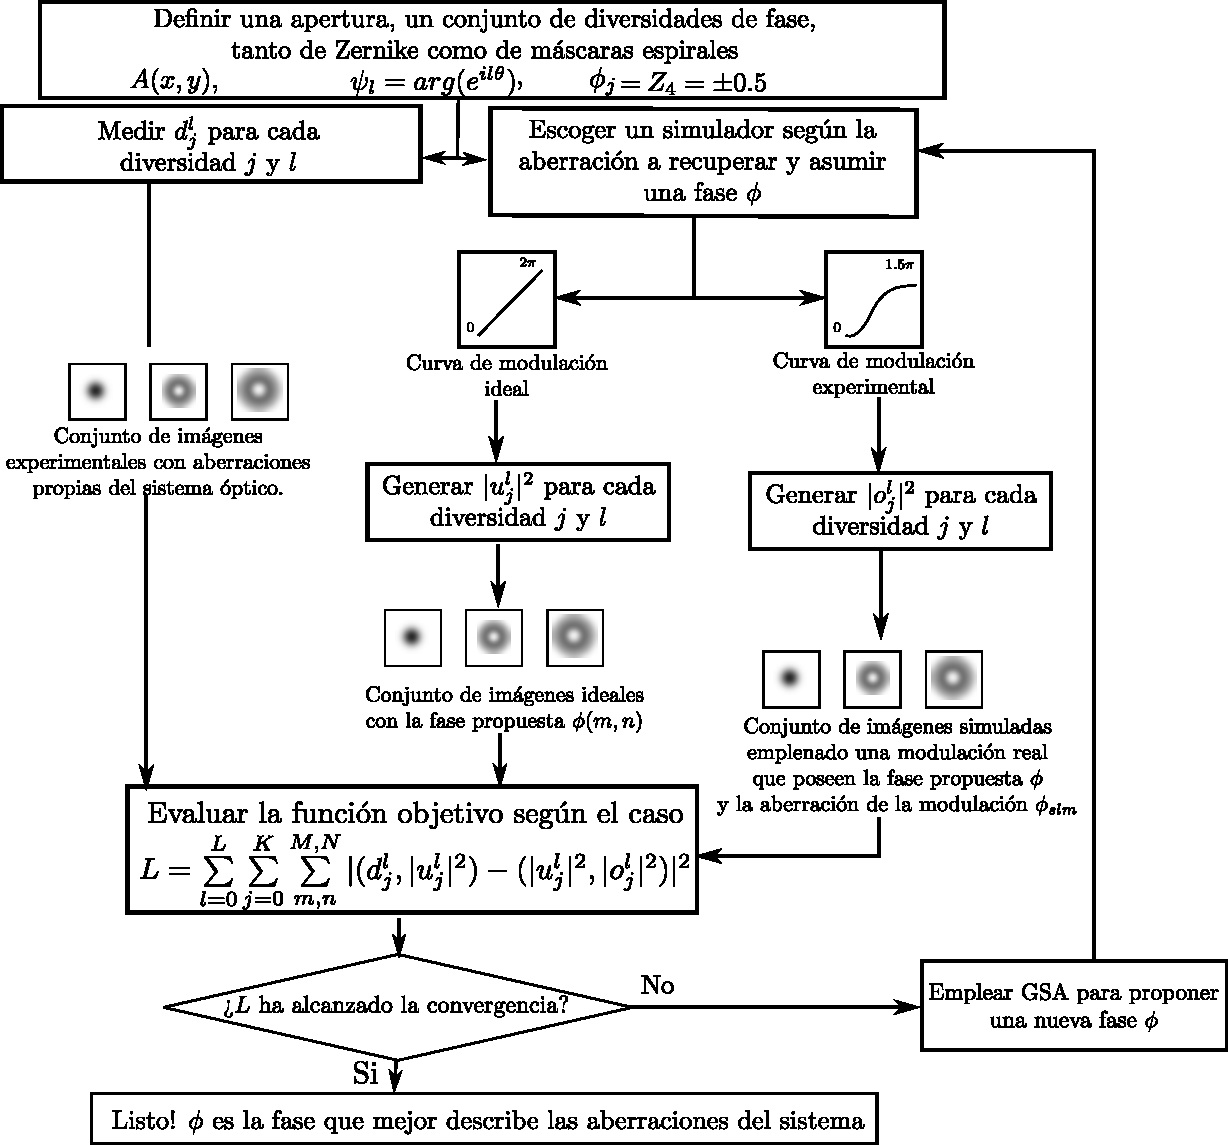
\includegraphics[width=\textwidth,keepaspectratio]{Caps/Imagenes/pdfluxadd.pdf}
  \caption{Diagrama de flujo de PD coherente con sus respectivas modificaciones.}
  \label{fig:pdfluxadd}
\end{figure}

%%
% Ecuaciones con el rótulo eqD.. pertenecen al capítulo de diversidad de fase
% con el róti eqV a vortices
%
\chapter{Implementaciones experimentales}
\label{cap:implementacion}

A lo largo de este capítulo se mostrarán algunas de las aplicaciones desarrolladas para la obtención de las curvas de modulación del SLM, la presentación de máscaras al SLM y la simulación de los OVs, elementos que de alguna manera han facilitado, o bien el trabajo experimental o, la implementación de PD coherente.\\

% y finalmente, el montaje experimental, centrándonos en la caracterización del SLM.\\

En la sección \ref{sec:slm_carac} se analizará uno de los métodos de caracterización de modulación en fase y amplitud para un SLM de transmisión y su ejecución en el laboratorio, además se especificarán las características del LC-2002 y por último, se presentará una interfaz que se desarrolló para generar y proyectar máscaras en el SLM. Finalmente en la sección \ref{sec:mont_exp} se mostrará y analizará el montaje experimental.

% Caracterizacion SLM -
% Generacion de OVs simulados -
%	-> Empleando curva SLM -
% Montaje experimental -
% PD Coherente -
%	-> PD1 -
%	-> PD2 -
% Presentació de mascaras al SLM -
% 

\section{Caracterización del modulador espacial de luz}
\label{sec:slm_carac}
%Dado que para nuestros objetivos se requiere de la curva de caracterización del SLM, en esta sección discutiremos cómo puede obtenerse esta. 
Anteriormente se mencionó que la modulación depende del estado de polarización de la luz, tanto a la entrada del SLM como a la salida de éste; es necesario entonces contar con un sistema generador-analizador de estados de polarización \cite{Campos2000, Iemmi2001, Malacara2007}. Esto se realiza por medio de una lámina retardadora de media longitud de onda (HWP: \textit{HWP: half-wave plate}), un polarizador y dos láminas retardadoras de un cuarto de longitud de onda (QWP:\textit{quarter-wave plate}) configurados como sea se muestra en la Fig. \ref{fig:genpol}.

\begin{figure}[!ht]
  \centering
    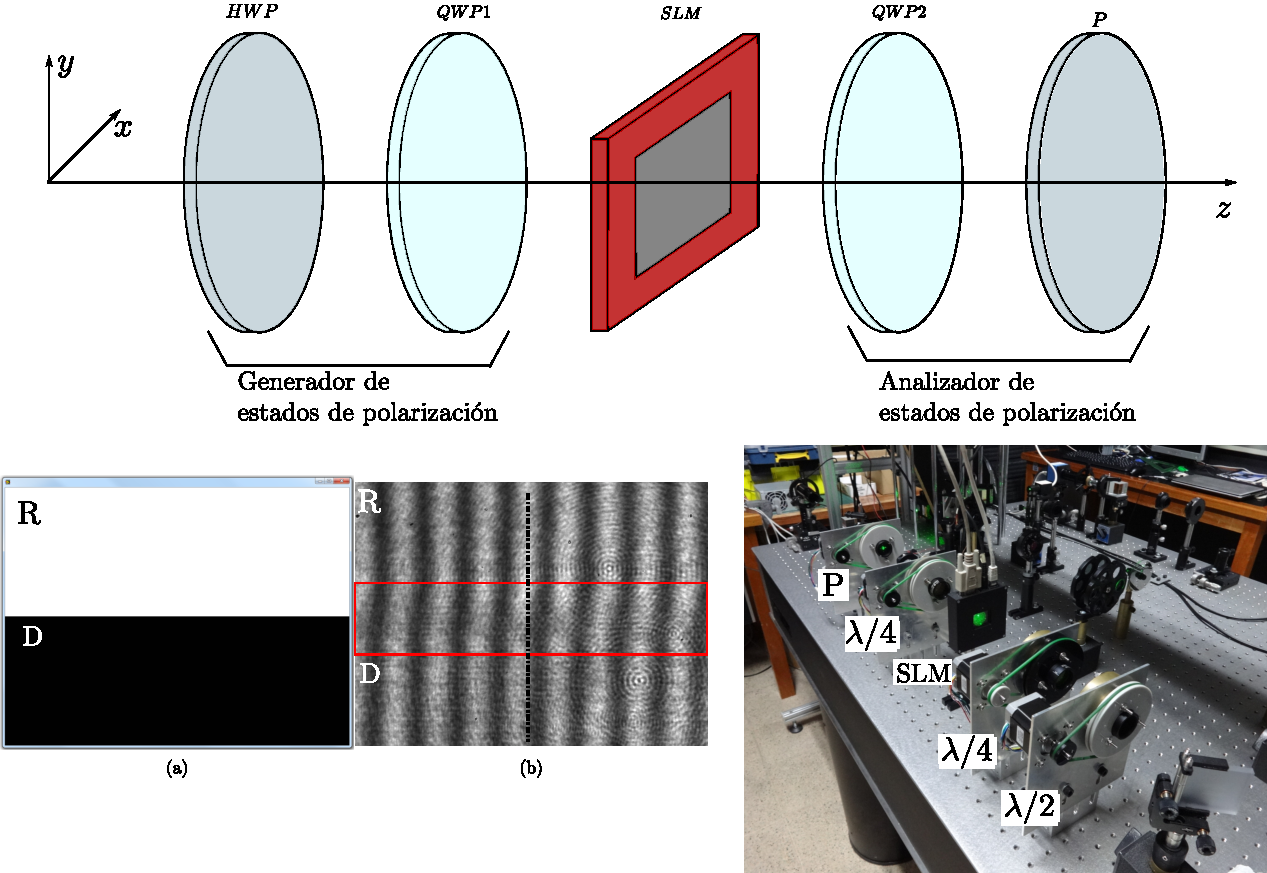
\includegraphics[width=\textwidth,keepaspectratio]{Caps/Imagenes/Gen-anPol.pdf}
  \caption{Estructura generador-analizador de estados de polarización para la caracterización de SLMs.}
  \label{fig:genpol}
\end{figure}

El generador de estados de polarización (PSG: \textit{polarization state generator}) se encarga de presentar el estado de polarización de la luz a la entrada del SLM, que puede ser lineal, circulares o elíptico, mientras que el analizador de estados de polarización (PSA: \textit{polarization state analyzer}) se encarga de analizar el estado de polarización a la salida del SLM. En conjunto, dadas las características de las moléculas de LC, según el estado de polarización puede haber una mayor o menor modulación de fase, amplitud o ambos. La caracterización del SLM se lleva a cabo a través de los resultados en intensidad medidos por un detector, en este caso, una cámara CCD, para diferentes estados de polarización, tanto en el analizador como en el generador de estados de polarización. La modulación en amplitud se determina a través del promedio de la intensidad medida \cite{Moreno2003, Ma2011}, mientras que la modulación en fase por su lado, se determina a través de un patrón de franjas interferométrico, en donde se divide el SLM en dos secciones, una de referencia y una en la cual se varía los niveles de gris en el SLM, el cambio en la fase produce entonces un desplazamiento del patrón de franjas en la sección donde se varían los niveles de gris con respecto a la sección referencia, como se muestra en la Fig.\ref{fig:faseslm}. \\

\begin{figure}[!ht]
  \centering
    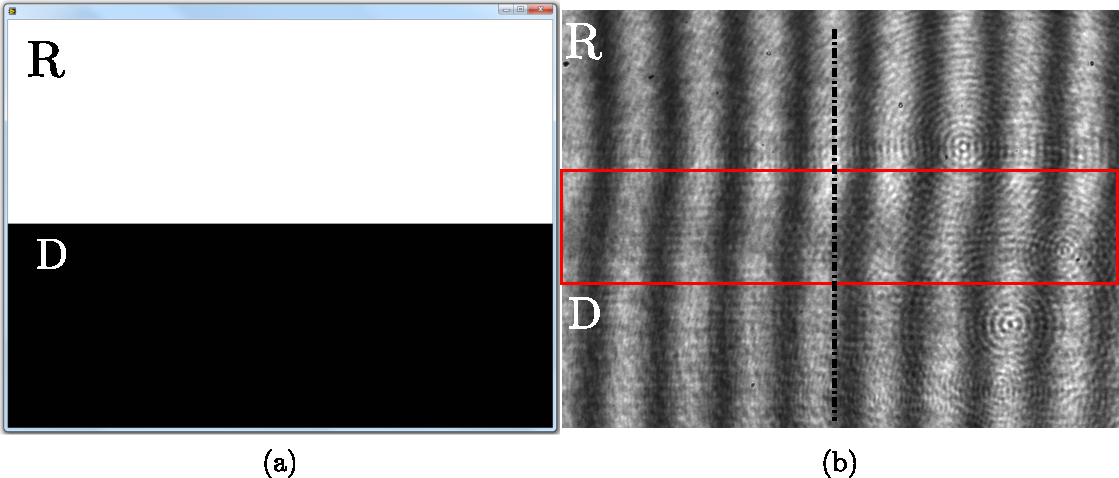
\includegraphics[width=14cm,keepaspectratio]{Caps/Imagenes/faseslm.pdf}
  \caption[Patrón de franjas para la determinación del corrimiento de fase en un sistema interferométrico.]{Patrón de franjas para la determinación del corrimiento de fase en un sistema interferométrico. (a) máscara dividida presentada al SLM, la sección R es la referencia y la sección D es en la que se varían los niveles de gris, y (b) patrón de franjas en el cual se desplaza la sección D a causa del cambio de fase producid por el SLM.}
  \label{fig:faseslm}
\end{figure}

Para llevar a cabo la caracterización, se diseñó un sistema compuesto por cuatro rotadores en donde cada uno de ellos se encarga de posicionar uno de los elementos ópticos; esto permite que la obtención de resultados experimentales sea de manera automática a través de una interfaz gráfica, en la cual solo es necesario ingresar qué estados se desean medir. Este sistema se muestra en la Fig. \ref{fig:rotadores}. Información detallada del proceso del modelo matemático que se sigue, resultados de la caracterización, hardware y software desarrollados puede encontrarse en la tesis de maestría de Santiago Echeverri \cite{EcheverriChacon2015}.

\begin{figure}[!ht]
  \centering
    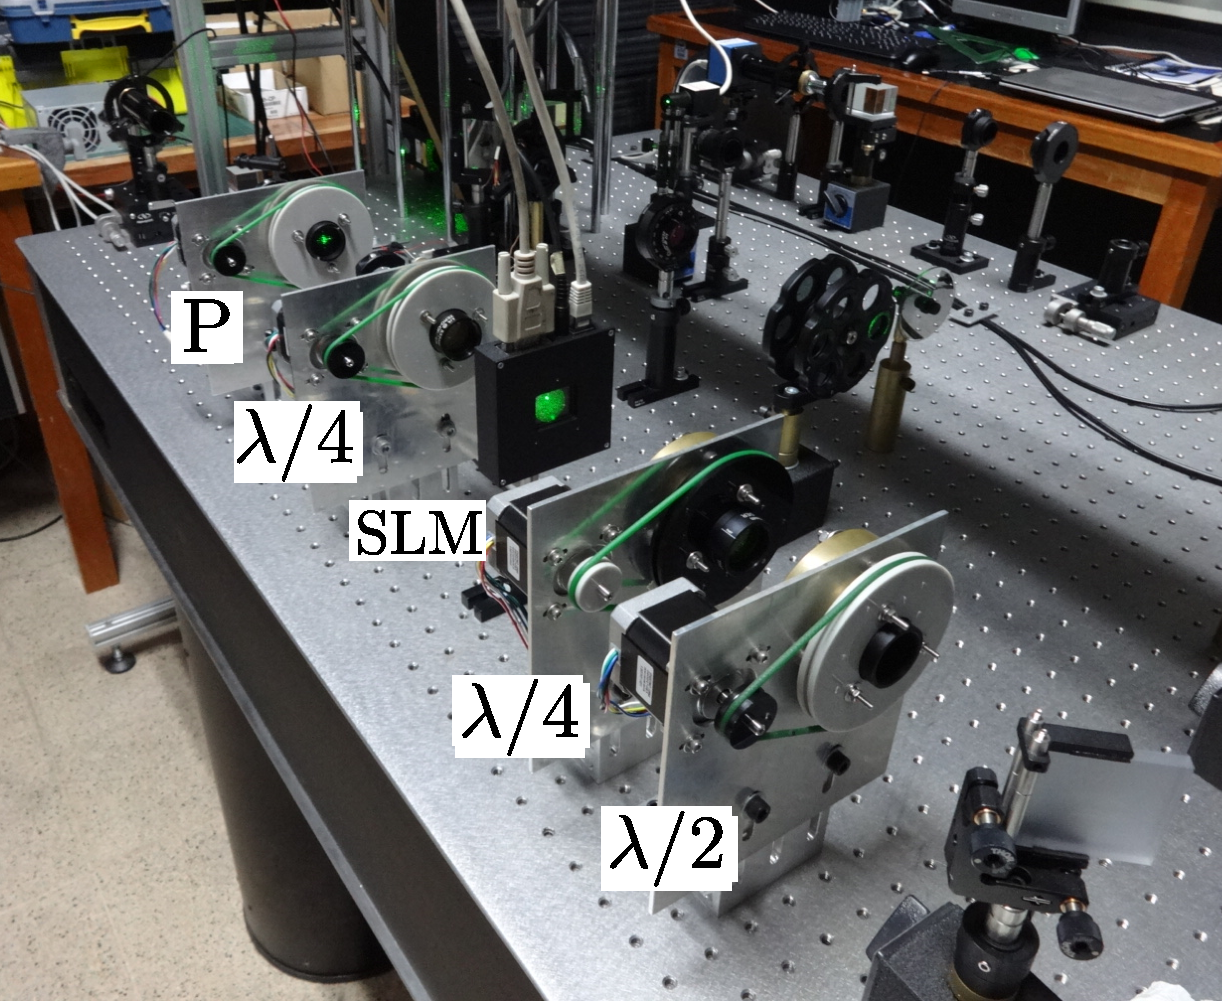
\includegraphics[width=12cm,keepaspectratio]{Caps/Imagenes/rotadores.pdf}
  \caption{Sistema de rotadores para la caracterización del SLM.}
  \label{fig:rotadores}
\end{figure}

El SLM que se emplea en este trabajo es un Holoeye LC-2002 (véase Fig. \ref{fig:lc2002}), el cual está basado en un microdisplay traslucido de LC y puede ser controlado electrónicamente vía computador\footnote{\url{http://www.rayscience.com/holoeye/LC2002_280.pdf}. }. En la Tabla \ref{tab:lc2002} se muestran las características técnicas.

\begin{figure}[!ht]
  \centering
    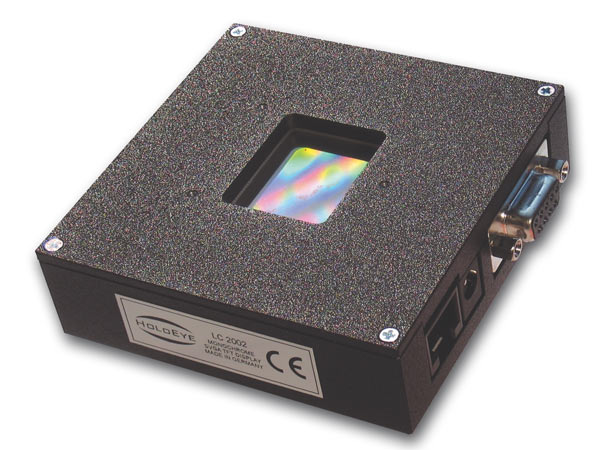
\includegraphics[scale=0.3]{Caps/Imagenes/lc2002.jpg}
  \caption[SLM HOLOEYE LC-2002.]{SLM Holoeye LC-2002. Imagen tomada de \small \url{http://holoeye.com/wp-content/uploads/2011/07/lc2002_spatial_light_modulator.jpg}}
  \label{fig:lc2002}		
\end{figure}



\begin{center}
\begin{table}
\centering
\begin{tabular}{|c|c|}
\hline 
Tipo de display & LC de transmisión \\ 
\hline 
Resolución & 800$\times$600 \\ 
\hline 
Tamaño del píxel & 32 $\mu$m \\ 
\hline 
Factor de llenado & $55\%$ \\ 
\hline 
Área activa & 21$\times$26mm \\ 
\hline 
Modulación de fase & $2\pi$ a 532nm \\ 
\hline 
\end{tabular} 
\caption{Características del LC-2002}
\label{tab:lc2002}
\end{table}
\end{center}

Para facilitar la generación y presentación de máscaras al SLM, se incorporaron las diferentes funciones que generan máscaras en una sola aplicación denominada ``SLM Mask Generator'', como se muestra en la Fig. \ref{fig:maskgen}. Esta se ha desarrollado en Matlab y se encuentra en proceso de registro de software ante la Dirección Nacional de Derecho de Autor.\\

\begin{figure}[!ht]
  \centering
	    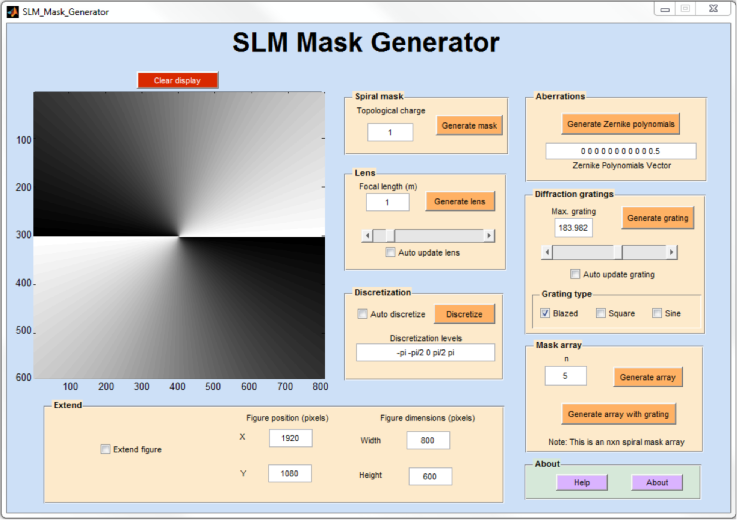
\includegraphics[width=\textwidth,keepaspectratio]{Caps/Imagenes/maskgen.png}
	\caption[Interfaz para la generación de máscaras.]{Interfaz para la generación de máscaras con diversas características para presentarse al SLM.}
	\label{fig:maskgen}
\end{figure}

La generación de una máscara espiral de fase se realiza mediante el ingreso de una carga topológica en la casilla ``Topological charge'' y posteriormente, haciendo click en el botón ``Generate mask'', con esto se dará una vista previa de la máscara como la que se muestra en el recuadro. A través de la opción ``Extend'' puede presentarse la máscara al SLM, esto debido a que cuando el SLM está conectado al computador funciona como una segunda pantalla y puede entonces cambiar el tamaño y la posición de la imagen a proyectar. A grandes rasgos, la aplicación permite simular diferentes tipos de elementos de fase como: aberraciones a partir de los polinomios de Zernike, redes de difracción de tres tipos e incluso, arreglos de máscaras espirales. En la Fig. \ref{fig:resmaskapp} se presenta el resultado para cuatro máscaras generadas con la aplicación.

%Para presentar las diferentes máscaras al SLM implementó una interfaz gráfica en MATLAB, que se muestra en la Fig.\ref{fig:maskgen}, la cual permite generar máscaras con diversas características, entre las cuales se tiene:

%\begin{itemize}
%	\item Genera máscaras espirales de cualquier carga topológica que son ajustables a la resolución del modulador espacial.
%	\item Extender las máscaras con una sección de posicionamiento y ajuste del tamaño, en donde se puede decidir la posición y dimensiones de la máscara a proyectar
%Permite superponer lentes de diferentes distancias focales a la máscara actual y posee una opción de actualización automática en caso de que se desee variar la distancia focal de manera dinámica. 
%	\item Puede discretizar las máscaras en niveles de gris, estos niveles permiten la creación de máscaras de dos o más niveles de gris, esta sección también la posibilidad de discretizar de manera automática. 
%	\item Genera aberraciones a partir de los polinomios de Zernike, en donde dado un vector de pesos se genera una superficie con la suma de las características de los pesos y se superpone a la máscara actual. 
%Produce redes de difracción de tres tipos: binarias, sinusoidales o diente de sierra, en las cuales se puede variar el periodo de manera dinámica.
%	\item Posee una sección para la generación de arreglos de nxn máscaras espirales y a estos arreglos puede añadirse redes de difracción.
%\end{itemize}



\begin{figure}[!ht]
  \centering
	    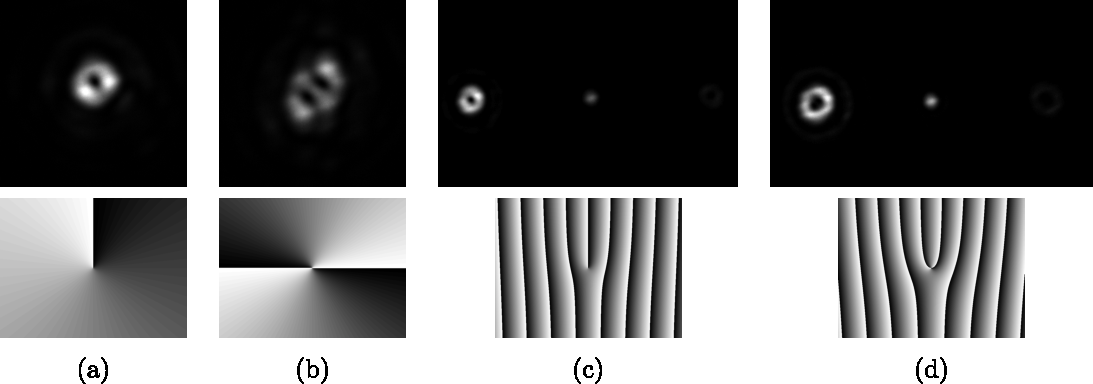
\includegraphics[width=\textwidth,keepaspectratio]{Caps/Imagenes/resmaskapp.pdf}
	\caption[Resultados de máscaras generadas con el ``SLM Mask Generator''.]{Resultados de máscaras generadas con el ``SLM Mask Generator''. (a) Máscara de fase espiral con carga topológica $l=1$, (b) máscara de fase espiral $l=2$, (c) red de difracción diente de sierra bifurcada con $l=1$ y (d) red de difracción diente de sierra bifurcada con $l=2$.}
	\label{fig:resmaskapp}
\end{figure}

%\section{Presentación de hologramas generados por computadora al modulador espacial de luz}

%Como el SLM también posee las características de un LCD, la presentación de las diferentes máscaras puede realizarse a través de una interfaz

%\section{Simulación de vórtices ópticos}
%\label{sec:gen_vor_sim}
%
%Ahora bien, puesto que PD coherente requiere de una estimación \textit{a priori} del objeto, lo que allí se hace es emplear un simulador de OVs, un diagrama de flujo de este se muestra en la Fig. \ref{fig:GenVor}a. El proceso que se sigue es en esencia el propuesto en la Eq.\ref{eqD1}, es decir, una convolución entre el plano objeto y la función de punto extendido. Puesto que en la propuesta de PD1 y PD2 se opta por modificar la simulación de forma tal que la fase que es añadida por la función pupila generalizada concuerde con los valores de modulación de fase real\footnote{Recordemos que las variaciones de intensidad se desprecian puesto que el estado de polarización es tal que las variaciones de intensidad son mínimas.} se añade un paso adicional a la simulación, en el cual los valores de fase son modificados para que estos correspondan a los valores de fase aportados por el SLM (Fig.\ref{fig:GenVor}b). Dado que queremos realizar una convolución, uno de los sistemas ópticos más empleado para ello ha sido el bien conocido correlador 4F.En este se siguen las siguientes etapas: se tiene un par de lentes cada una con distancia focal $f$, primero se ubica una de ellas a una distancia $f$ del plano objeto, de forma que a $2f$ de se genere la transformada de Fourier del plano objeto. En este punto se añade la PSF del sistema, que en nuestro caso corresponde a la información de fase añadida por el SLM. A continuación se ubica la segunda lente a una distancia de $3f$ con respecto al plano objeto, esta se encargará de realizar una segunda transformadad de Fourier del producto entre la PSF y la transformada del plano objeto, de forma que a la salida lo que tendremos de acuerdo a la Eq.\ref{eqD1} es la convolución entre la  PSF y el plano objeto.
%
%\begin{figure}[!ht]
%  \centering
%  	\subfigure[Sin modulación real.]{
%	    \includegraphics[scale=1]{Caps/Imagenes/GenVor.pdf}}
%	\quad
%	\subfigure[Con modulación real.]{
%	    \includegraphics[scale=1]{Caps/Imagenes/GenVorMod.pdf}}
%	\caption{Simulación de OVs.}
%	\label{fig:GenVor}
%\end{figure}


%\begin{figure}[!ht]
%  \centering
%    \includegraphics[scale=1]{Caps/Imagenes/GenVorMod.pdf}
%  \caption{Diagrama de flujo de la simulación de un OV modificado para emplear la}
%  \label{fig:montaje}
%\end{figure}

\section{Montaje experimental}
\label{sec:mont_exp}

%Un esquema del montaje se presenta en la Fig. \ref{fig:montaje}, el cual está compuesto por un interferómetro Mach-Zehnder que en uno de sus brazos ha sido ubicado un correlador 4F. Además, en el 4F se ha ubicado el sistema PSG-PSA de forma que con uno de los brazos del intereferométro se hace imagen de un punto objeto y  se añade el SLM que se encarga de presentar los CGH. La Fig.\ref{fig:montexp} es una toma del montaje físico.

%Un esquema del montaje se presenta en la Fig. \ref{fig:montaje}, como fuente de iluminación se emplea un láser de estado sólido con una longitud de onda de $532$nm, con polarización vertical y modo $TEM_{0,0}$. Primero se ubica un polarizador con recubrimiento delgado a base de nanopartículas con alta relación de extinción ($10000:1$) de referencia LPVISB050 fabricado por THORLABS; este polarizador se utiliza ya que los láseres de estado sólido pueden tener una polarización elíptica. A continuación se sitúa un filtro de densidad neutra que permite modificar la intensidad y a través de un conjunto de espejos de primera superficie, se lleva el haz hasta un filtro espacial compuesto por un objetivo de $10\times$ y un ``pinhole'' de $5\mu $m, que permite filtrar las altas frecuencias y producir un haz Gaussiano. Luego se ubica una lente colimadora con distancia focal de $10$cm, seguido por un divisor de haz no polarizado de referencia $49-004$ fabricado por Edmund Optics, desde aquí se genera entonces un interferómetro Mach-Zehnder. En el brazo objeto se ubica una primera lente tiene una distancia focal de $10$cm, de forma que en el plano focal de dicha lente tendremos el plano objeto, a partir de este se da entonces el sistema formado de imagen 4F. Se ubica una segunda lente de forma que a distancia focal está colocado el SLM, garantizando que las fases introducidas por el SLM están en un plano de Fourier. Antes de este está el sistema PSG conformado por una lámina de cuarto de longitud de onda de referencia WPQ10M-532 de THORLABS y una lámina de media longitud de onda de referencia WPH10M-532 del mismo fabricante. Después del SLM está el PSA conformado por un polarizador y una lámina de cuarto de onda. Se ubica una segunda lente de forma que desde el SLM hasta el plano imagen hay $2f$ y allí se ubica un ocular mar Newport con aumento de $10\times$ acoplado a una cámara CCD marca Imaging Source modelo DMK 41BU02.H con una resolución de $1280 \times 960$. 

Un esquema del montaje se presenta en la Fig. \ref{fig:montaje}, como fuente de iluminación se emplea un láser de estado sólido con una longitud de onda de $532$nm, con polarización vertical y modo $TEM_{0,0}$. Primero se ubica un polarizador con recubrimiento delgado a base de nanopartículas con alta relación de extinción ($10000:1$) de referencia LPVISB050 fabricado por THORLABS; este polarizador se utiliza ya que los láseres de estado sólido pueden tener una polarización elíptica. A continuación se sitúa un filtro de densidad neutra que permite modificar la intensidad y a través de un conjunto de espejos de primera superficie, se lleva el haz hasta un filtro espacial compuesto por un objetivo de $10\times$ y un ``pinhole'' de $5\mu $m, que permite filtrar las altas frecuencias y producir un haz Gaussiano. Luego se ubica una lente colimadora con distancia focal de $10$cm, seguido por un divisor de haz no polarizado de referencia $49-004$ fabricado por Edmund Optics. En el brazo objeto se ubica una primera lente, con una distancia focal de $10$cm, de forma que en el plano focal de dicha lente tendremos el plano objeto. Se ubica una segunda lente de forma que a distancia focal está situado el SLM, garantizando que las fases introducidas por el SLM están en un plano de Fourier. Antes de este está el generador de estados de polarización conformado por una lámina de cuarto de longitud de onda de referencia WPQ10M-532 de THORLABS y una lámina de media longitud de onda de referencia WPH10M-532 del mismo fabricante. Después del SLM está el analizador de estados de polarización conformado por un polarizador y una lámina de cuarto de onda. Se ubica una segunda lente de forma que desde el SLM hasta el plano imagen hay $2f$ y allí se ubica un objetivo de microscopio Newport con aumento de $20\times$ acoplado a una cámara CCD marca Imaging Source modelo DMK 41BU02.H con una resolución de $1280 \times 960$. 


\begin{figure}[!ht]
  \centering
    \includegraphics[width=\textwidth,keepaspectratio]{Caps/Imagenes/Montaje.pdf}
  \caption{Esquema del montaje experimental.}
  \label{fig:montaje}
\end{figure}



\begin{figure}[!ht]
  \centering
    \includegraphics[width=\textwidth,keepaspectratio]{Caps/Imagenes/montexp.JPG}
  \caption{Montaje experimental.}
  \label{fig:montexp}
\end{figure}


%
\chapter{Resultados}
\label{cap:resultados}


% Simulación de vórtices ópticos
%	-> ideals
%	-> con curv mod
%
% Caracterización de la curva d emodulación
%
% Diversidad de fase coherente
%	-> Pd coherente
%	-> Pd1
%	-> Pd2
%	-> Pd1+Pd2
%	-> Objeto de fase

\section{Caracterización de modulador espacial de luz LC-2002}
\label{sec:carac_slm}

Como se planteó en la Sección \ref{sec:slm} según el estado de polarización de la luz tanto a la entrada como a la salida del SLM, puede darse una mayor o menor modulación de fase y/o amplitud, en este caso, nos centraremos en aquellos estados donde o bien la tramitancia se mantiene constante ante la variación de niveles de gris del SLM (aplicación de campo eléctrico sobre el dispositivo), o bien los cambios de fase sean lo más cercano posible a $2\pi$. De las diversas curvas de modulación obtenidas hubo tres casos de mayor interés resumidos en la Tabla \ref{tab:mods}. Los ángulos y estados de polarización del sistema generador-analizador de estados de polarización se muestran en la Tabla \ref{tab:angulos1}.\\

\begin{table}[!ht]
\centering
\begin{tabular}{|c|c|c|}
\hline 
\rule[-1ex]{0pt}{2.5ex} Estado & Modulación en fase [rad.] & Variación de la tramitancia [$\%$]\\ 
\hline 
\rule[-1ex]{0pt}{2.5ex} $\omega_1$ & $1.8\pi$ & $\approx 90$ \\ 
\hline 
\rule[-1ex]{0pt}{2.5ex} $\omega_2$ & $1.4\pi$ & $\approx 12$ \\ 
\hline 
\rule[-1ex]{0pt}{2.5ex} $\omega_3$ & $1.6\pi$ & $\approx 30$ \\ 
\hline 
\end{tabular} 
\caption{Características de la modulación en los estados $\omega_1$, $\omega_2$ y $\omega_3$.}
\label{tab:mods}
\end{table}

%\begin{itemize}
%\item Modulación en fase de $1.8\pi$ y $90\%$ de variación en la tramitancia, $\omega_1$.
%\item Modulación en fase de $1.4\pi$ y $12\%$ de variación en la tramitancia, $\omega_2$.
%\item Modulación en fase de $1.6\pi$ y $30\%$ de variación en la tramitancia, $\omega_3$.
%%\item $\omega_2$ que presenta una modulación en fase de $1.4\pi$ y $12\%$ de variación en la tramitancia.
%%\item $\omega_3$ que presenta una modulación en fase de $1.6\pi$ y $30\%$ de variación en la tramitancia.
%\end{itemize}


En el caso de $\omega_1$, mostrado en la Fig. \ref{fig:curva1}, se logra la máxima modulación en fase posible para el SLM, siendo esta muy cercana a $2\pi$ (Fig. \ref{fig:curva1}(a)), sin embargo, la modulación en amplitud (Fig. \ref{fig:curva1}(b)) supera el $80\%$ para los niveles de gris ubicados entre $160$ y $180$. Ahora bien, podría pensarse que es posible emplear aquellos niveles de gris donde el cambio de fase es mayor, de forma que sea posible evadir los efectos de los cambios de amplitud, pero de acuerdo a las curvas obtenidas, se observa que la mayor modulación de amplitud se ubica en los niveles de gris en donde la fase presenta una mayor variación y por tanto, se producirá una diferencia de amplitudes entre diferentes puntos de la máscara espiral de fase cuando esta sea presentada al SLM, produciendo zonas con  baja tramitancia. En el caso de $\omega_2$, que se presenta en la Fig. \ref{fig:curva3}, a diferencia de lo que sucede en $\omega_1$, en este el cambio de amplitud es menor al $12 \%$ (Fig. \ref{fig:curva3}(a)); sin embargo, la modulación de fase máxima es de alrededor de $1.4\pi$ (Fig. \ref{fig:curva3}(b)) y en los niveles de gris próximos se dan saltos de fase tales que propician que la curva sea abrupta, esto se repite a lo largo de los 256 niveles de gris. Estas irregularidades en el cambio de fase no son deseadas para la generación de OVs, dado que la calidad de los OVs mejora cuando su máscara espiral de fase tiene un comportamiento \textit{suave}. En el caso de $\omega_3$, presentado en la Fig. \ref{fig:curva2}, si bien es cierto que la intensidad varía alrededor del $30\%$, la modulación en fase es de $1.6\pi$ y la curva se comporta de manera \textit{suave}.\\


\begin{table}[!ht]
 \centering
    \includegraphics[scale=1.0]{Caps/Imagenes/angulosCurva1.pdf}
  \caption{Ángulos y estados de polarización para $\omega_1$, $\omega_2$ y $\omega_3$.}
  \label{tab:angulos1}
\end{table}

% que denominaremos caso 1, caso 2 y caso 3, y respectivamente corresponden a: $2\pi$ de modulación en fase, variación de intensidad menor al $10\%$ y en fase mayor a $\pi$ y variación de intensidad menor al $30\%$ con modulación en fase de $1.6\pi$. Los ángulos en del PSG y PSA se encuentran en la tabla \ref{tab:angulos1}. \\


%En el caso 1 ocurre algo interesante y es que el SLM logra la modulación máxima indicada por el fabricante, siendo esta de $2\pi$, por otro lado, la modulación en amplitud supera el $80\%$ para los niveles de gris ubicados entre 160 y 180, como se muestra en la Fig.\ref{fig:curva1}. Ahora bien, podría pensarse que es posbile emplear aquellos niveles de gris donde es da el mayor cambio de fase, de forma que sea posible evadir los efectos sobre la intensidad, pero si se observan las gráficas, es fácil ver que la mayor modulación de la intensidad se da en los niveles de gris en donde la fase varía, por lo tanto, hay que considerar que se presentará una diferencia de intensidad cuando la SPM sea presentada al SLM.


% sucede lo contrario al primero, en este el cambio de amplitud es menor al $10 \%$, podríamos decir que se mantiene constante (Fig. \ref{fig:curva2}), aunque la modulación de fase de alrededor de $1.4\pi$, pero a diferencia del caso anterior, los cambios de fase entre niveles de gris próximos propician que la curva sea abrupta a lo largo de los 256 niveles de gris.

\begin{figure}[!ht]
  \centering
    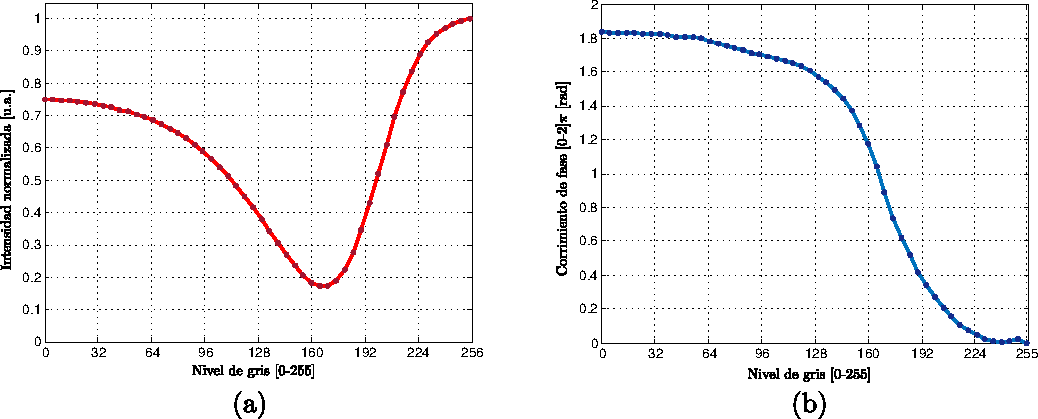
\includegraphics[width=\textwidth,keepaspectratio]{Caps/Imagenes/curva1.pdf}
  \caption[Curva de modulación de amplitud y fase del SLM para el estado $\omega_1$.]{Curva de modulación de amplitud y fase del SLM para el estado $\omega_1$. ((a) Curva de modulación de amplitud, donde se observan variaciones en amplitud de hasta un $80\%$ y (b) curva de modulación de fase donde se obtienen cambios máximos de $1.8\pi$).}
  \label{fig:curva1}
\end{figure}

\begin{figure}[!ht]
  \centering
    \includegraphics[width=\textwidth,keepaspectratio]{Caps/Imagenes/curva3.pdf}
  \caption[Curva de modulación de amplitud y fase del SLM para el estado $\omega_2$.]{Curva de modulación de amplitud y fase del SLM para el estado $\omega_2$. ((a) Curva de modulación de amplitud con una variación menor al $12\%$ y (b) curva de modulación de fase donde se obtienen un cambio máximo de $1.4\pi$ con discontinuidades entre niveles de gris).}
  \label{fig:curva3}
\end{figure}

\begin{figure}[!ht]
  \centering
    \includegraphics[width=\textwidth,keepaspectratio]{Caps/Imagenes/curva2.pdf}
  \caption[Curva de modulación de amplitud y fase del SLM para el estado $\omega_3$.]{Curva de modulación de amplitud y fase del SLM para el estado $\omega_3$. ((a) Curva de modulación de amplitud con una variación de un $30\%$ y (b) curva de modulación de fase donde se obtienen un cambio máximo de $1.6\pi$).}
  \label{fig:curva2}
\end{figure}

%este estado podría ser empleado para generar OVs. La mayor desventaja en este punto es que la fase presenta un comportamiento más abrupto que el caso anterior.


De los resultados obtenidos para los estados $\omega_1$, $\omega_2$ y $\omega_3$ empleando el LC-2002, podemos concluir con respecto a su modulación que:

\begin{itemize}
\item No presenta un comportamiento lineal para la variación de fase con respecto a los niveles de gris, es decir, que la modulación en fase no se comporta de manera lineal ante la presencia de un campo eléctrico.
\item Aunque sea baja la modulación en amplitud, en los niveles de gris en los cuales se dan las variaciones de fase hay también asociada una diferencia en la amplitud.
\item Como consecuencia del ítem anterior, se comprueba que efectivamente, la modulación de fase y amplitud se encuentran acopladas y dependen de los estados de polarización del sistema generador-analizador de estados de polarización.
\end{itemize}

%En el caso de $\omega_3$, que se muestra en la figura \ref{fig:curva3}, si bien es cierto que la intensidad varía alrededor del $30\%$, la modulación en fase es cercana a los $1.6\pi$ y la curva se comporta de manera \textit{suave}, es decir, el salto de fase entre niveles de gris vecinos es aproximadamente constante, aunque como tal, ninguna de las curvas no es lineal.
%en cuanto a la intensidad hay una variación de alrededor del $30\%$, pero en la fase además de tenerse una modulación de fase cercana a los $1.6\pi$ y la curva se comporta de manera \textit{suave}, es decir, los cambios de fase entre niveles de gris vecinos son aproximadamente, aunque como tal, la curva no es lineal. Con estas tres modulaciones se generaron entonces OVs y de allí se escogió como punto de trabajo el ofrecido por la curva tres. A continuación, analizaremos los OVs que se producen en cada uno de los puntos de trabajo propuestos.

%Si bien es cierto que los tres casos presentados poseen características que pueden ser ventajosas para generar OVs, es difícil concluir \textit{a priori} cuál de las curvas es la que mejor se presta para su fin, por ello, a continuación se mostrarán los OVs que se generan en cada uno de los casos.

Si bien es cierto que los tres casos presentados poseen características que pueden ser favorables para generar OVs, es difícil concluir \textit{a priori} cuál de estas presenta un mejor comportamiento en la generación de OVs; por ello, a continuación analizaremos los OVs que se obtienen en cada caso.

%Con estas tres modulaciones se generaron entonces OVs y de allí se escogió como punto de trabajo el ofrecido por la curva tres. A continuación, analizaremos los OVs que se producen en cada uno de los puntos de trabajo propuestos.

%En este caso, aunque la variación en amplitud es de alrededor de un $30\%$, la variación de fase es 

%A continuación se mostrarán las curas de variación de fase e intensidad para cada uno de los casos. El primero corresponde a una modulación de $2\pi$ en fase, pero este resultado sea óptimo, la variación en intensidad es de alrededor de un $80\%$ y a causa de esto, no es recomendable emplear esta modulación.

%Hay otros dos estados en los cuales las variaciones de intensidad es menor a $20\%$, la desventaja de estos es que la modulación en fase es de $1.3\pi$ y $1.5\pi$.

\section{Vórtices ópticos experimentales}
\label{sec:vor_opt_expe}
%\section{Selección del punto de trabajo}

%Una vez se han definido los posibles puntos de trabajo (estados PSG-PSA), se procede a generar OVs con cada uno de los casos, recordemos que una de las ventajas de emplear SLMs es que permite presentar SPMs de manera programable mediante CGHs. La Fig.\ref{fig:curvaovs} muestra los resultados obtenidos para cada una de los tres puntos de trabajo planteados en la sección \ref{sec:carac_slm}, allí, el RMS promedio corresponde al error RMS pixel a pixel entre un OV generado por un sistema óptico limitado por difracción con el OAM correspondiente y el OV en cuestión. 

%, se procede a generar OVs con cada uno de los casos, recordemos que una de las ventajas de emplear SLMs es que permite presentar SPMs de manera programable mediante CGHs. La Fig.\ref{fig:curvaovs} muestra los resultados obtenidos para cada una de los tres puntos de trabajo planteados en la sección \ref{sec:carac_slm}, allí, el RMS promedio corresponde al error RMS pixel a pixel entre un OV generado por un sistema óptico limitado por difracción con el OAM correspondiente y el OV en cuestión. 


%De la Fig.\ref{fig:curvaovs} es evidente que el caso 1 produce los OVs de menor calidad, de hecho, podría explicarse que la mayor parte de la energía se encuentra concentrada a causa de la alta modulación en amplitud, que produce que los OVs sean anisotrópicos. Analizando el caso dos y tres, visualmente es fácil concluir que ambos presentan una mejora en la calidad de los OVs que se producen. Ahora bien, para determinar cuál de los dos es mejor, se procedió a tomar el error RMS entre el OVs que producen y uno que se generaría en un sistema óptico limitado por difracción, al final, el mejor punto de trabajo será el que obtenga el menor error. De esto se concluyó que el mejor estado corresponde al caso tres y gracias a que conocemos la curva de modulación, podemos simular los efectos que esta curva produce en la generación de OVs. En la siguiente sección analizaremos los efecto de la modulación no lineal y menor a $2\pi$ sobre los OVs.

Una vez se han definido los estados de polarización para generar OVs ($\omega_1$, $\omega_2$ y $\omega_3$), se procede a obtener resultados experimentales para cada uno de dichos estados. Para ello se emplean máscaras de fase espiral con cargas topológicas $l=\pm 1$ ya que tenemos la ventaja de poder modificar de manera dinámica la máscara de fase espiral gracias a las características del SLM, con ello se obtuvieron los resultados presentados en la Fig. \ref{fig:curvaovs}.

\begin{figure}[!ht]
  \centering
    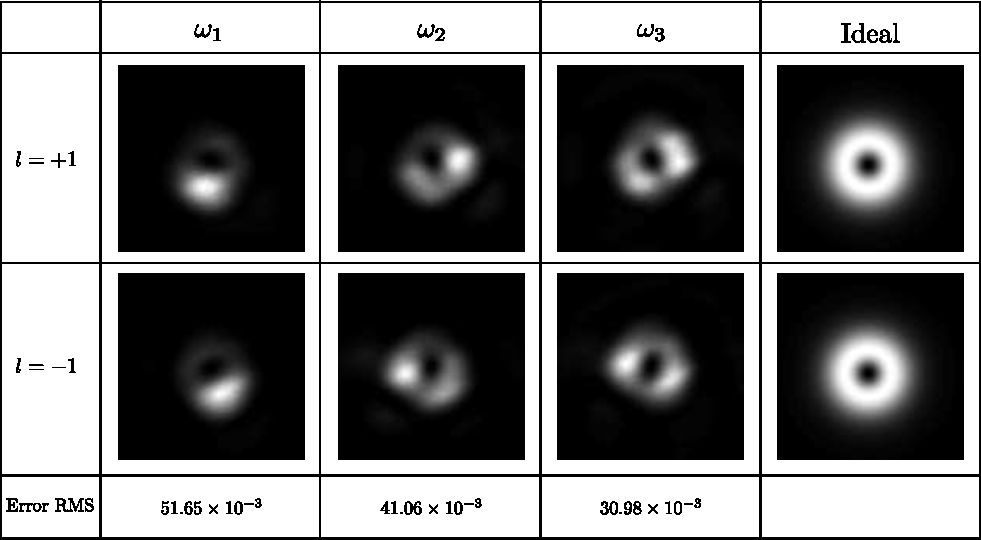
\includegraphics[width=\textwidth,keepaspectratio]{Caps/Imagenes/ovcurvas.pdf}
  \caption[Comparación de los OVs generados experimentalmente a partir de los estados $\omega_1$, $\omega_2$ y $\omega_3$.]{Comparación de los OVs generados experimentalmente a partir de los estados $\omega_1$, $\omega_2$ y $\omega_3$, con un OV producido por un sistema óptico limitado por difracción con modulación de fase lineal de $2\pi$.}
  \label{fig:curvaovs}
\end{figure}

El criterio usado para seleccionar el mejor estado, y por consiguiente, la mejor curva de modulación para generar OVs, fue el cálculo del error medio cuadrático (RMS: \textit{root mean square}) de la diferencia entre un OV ideal y el obtenido experimentalmente; definiendo el error $E$ como,
\begin{equation}
	E = \sqrt{\frac{1}{MN} \sum\limits_{n,m}^{M,N} |d(m,n)-u(m,n)|^2},
\end{equation}
donde $(m,n)$ representa cada uno de los píxeles en las imágenes obtenidas, $d(m,n)$ la imagen experimental y $u(m,n)$ un OVs ideal es un OV simulado libre de aberraciones, es decir, generado a través de un sistema óptico limitado por difracción con una modulación de fase lineal de $2\pi$. De la Fig. \ref{fig:curvaovs} se evidencia que el estado $\omega_1$ produce los OVs de menor calidad; visualmente, la mayor parte de la luz se encuentra concentrada en una región. Este hecho podría explicarse si analizamos la modulación en amplitud del estado, debido a que una zona el SLM posee una tramitancia menor al $20\%$, es de esperar que toda la energía se concentre en aquellos puntos donde la modulación de amplitud es constante y hay una máxima tramitancia. \\

Los estados $\omega_2$ y $\omega_3$ presentan un comportamiento similar y una mejora en la calidad de los OVs generados con respecto a $\omega_1$, para determinar cuál de estos genera el OV con mayor calidad se empleó un criterio basado en error RMS resultante de la comparación de las intensidades producidas por cada estado con los OV producidos por un sistema óptico limitado por difracción con modulación de fase lineal de $2\pi$, y como se muestra en la Fig. \ref{fig:curvaovs} y en la Tabla \ref{tab:estadosgenov}, son aquellos OVs producidos por el estado $\omega_3$ los que más se aproximan a OVs ideales. 

\begin{table}[!ht]
\centering
\begin{tabular}{|c|c|}
\hline 
Estado para la generación & Error RMS comparado con un OV ideal \\ 
\hline 
$\omega_1$ & $51.65 \times 10^{-3}$ \\ 
\hline 
$\omega_2$ & $41.06 \times 10^{-3}$ \\ 
\hline 
$\omega_3$ & $30.98 \times 10^{-3}$ \\ 
\hline 
\end{tabular} 
\caption{Errores obtenidos con los OVs producidos para los estados $\omega_1$, $\omega_2$ y $\omega_3$}
\label{tab:estadosgenov}
\end{table}


De los resultados obtenidos en esta sección, concluimos que para la generación experimental de OVs:

\begin{itemize}
\item Una modulación de fase cercana a $2\pi$ no necesariamente garantiza OVs de buena calidad, también es necesario considerar el efecto de la modulación en amplitud.
\item Una tramitancia constante con una modulación de $1.4\pi$ puede no ser el mejor estado de generación de OVs aunque la amplitud sea casi constante para todos los niveles.
\item Debe haber un compromiso entre la modulación en fase y amplitud que propicie generar OVs de una calidad razonable.
\end{itemize}



%Ahora que hemos determinado los estados de polarización y por consiguiente la curva de modulación en fase con la cual se generarán OVs, simularemos los efectos de esta modulación cuando se 
%
% los cuales se generarán los OVs, podemos proceder a simular los OVs que produce un sistema óptico limitado por difracción cuando posee una modulación en fase experimental.
%solo en los niveles de gris donde la modulacion de amplitud es relativamente constante y alta, es decir, donde la tramitancia se aleja de cero

%En el caso uno, se observa que si bien la modulación en fase es cercana a la ideal, las variación en intensidad produce que los OVs sean asimétricos. Para el caso dos, cualitativa y cuantitativamente hay una mejora en 
%Pero es claro que de los tres, el que mejor genera OVs es el caso tres y por tanto este fue el más empleado a lo largo del proyecto.
%Una vez se tiene un punto de trabajo, se procede a ubicar los diversos elementos ópticos en los ángulos requeridos y a partir, se presenta una máscara espiral de fase al SLM, de forma que éste actúa como una SPP programable mediante CGHs. Con la curva 

%Ahora que conocemos la curva de modulación, se podemos proceder a simular la modulación características en el punto de trabajo y con ello, implementar las modificaciones deseadas sobre PD coherente.
%- mostrar los Ovs con cada curva de modulacion 
%- mostrar el error rms entre cada uno de los casos
%- definir que dado el punto de trabajo el siguiente paso es simular las propiedades del slm de forma que se puedan simular los ovs producidos por un sistema limitado por difraccion en el slm


\section{Simulación de vórtices ópticos con curva de modulación experimental}
\label{sec:sim_vor_mod_exp}

%Con la implementación de un simulador de OVs a partir de la modulación real, como se mencionó en la sección \ref{sec:gen_vor_sim} se simularon OVs producidos por un sistema limitado por difracción con la modulación real para las cargas topológicas $\pm 1$, como se muestra en la figura \ref{fig:simvor}, en donde el error RMS está referido a los resultados experimentales, es decir, qué tan bien reproduce el modelo los resultados experimentales. Allí, cuando se generó la SPM, se modificó esta de forma tal que el salto fase que debe introducir cada punto, se reemplaza por el valor de fase real, es decir, el introduce el SLM. Ahora bien, sobe la SPM hay dos consecuencias directas al reemplazar los valores de modulación, estas son: perdida de la linealidad y limitación en la modulación máxima. Si bien cuando se simulan OVs que produce un sistema limitado por difracción, la máscara es lineal y alcanza valores de $2\pi$, aquí por el contrario, la máscara sigue la forma de la curva de modulación y de hecho, alcanza un valor máximo de $1.6\pi$, de esto se esperaría que cuando se simulen los OVs se obtenga un resultado más aproximado al experimental.

% y $\pm2$ y con esto, se pudo comparar el error RMS que se da entre los OVs generados en un sistema limitado por difracción con un SLM ideal, en un sistema limitado por difracción con un SLM real y los obtenidos de forma experimental. Ahora bien, para el caso de OVs caga topológica $1$, cualitativamente se puede observar que el generador de OVs basado en la CMR representa con mayor precisión (determinada por el error RMS) los OVs obtenidos en el sistema experimental.
Hasta el momento conocemos la curva de modulación de fase dada para el estado $\omega_3$ (referirse a la Fig. \ref{fig:curva2}); ahora queremos simular los OVs que produce un sistema óptico limitado por difracción cuando la máscara espiral de fase se produce con la modulación experimental del SLM. Esto se ejemplifica en la Fig. \ref{fig:mascaras}, cuando tenemos un SLM ideal, su modulación en fase es lineal y tiene un valor máximo de $2\pi$ (Fig. \ref{fig:mascaras}(a)), por ende, se produce una máscara espiral ideal que azimutalmente tiene la forma de la curva de modulación (Fig. \ref{fig:mascaras}(b)). Si tenemos la curva de modulación experimental (Fig. \ref{fig:mascaras}(c)), esta además de no ser lineal posee un valor de fase máximo de $1.6\pi$ y por tanto, la máscara espiral producida tiene la forma presentada en la Fig. \ref{fig:mascaras}(d). 

\begin{figure}[!ht]
  \centering
    \includegraphics[width=9cm,keepaspectratio]{Caps/Imagenes/mascaras.pdf}
  \caption[Comparación entre una máscara espiral ideal y experimental.]{Comparación entre una máscara espiral producida por un SLM con modulación de fase ideal y la máscara espiral producida por un SLM con modulación de fase experimental. ((a) Curva de modulación de fase ideal, (b) máscara de fase espiral ideal, (c) curva de modulación de fase experimental y (d) máscara de fase espiral producida por la modulación experimental).}
  \label{fig:mascaras}
\end{figure}

De esta forma, en la simulación de la generación de OVs hemos reemplazado la máscara espiral de fase ideal, con la máscara espiral de fase experimental, es decir, hemos agregado la modulación de fase de nuestro SLM a la simulación de un OV producido por un sistema óptico limitado por difracción, y de acuerdo a la Fig. \ref{fig:PD012}, en la Sección \ref{sec:pd12}, esto corresponde a $o_j^l$, cuando la diversidad de aberración $j=0$. Recordemos también que si simulamos la generación de un OV a partir de una modulación ideal y un sistema óptico limitado por difracción, obtenemos $u_j^l$. La diferencia entre $u_j^l$ y $o_j^l$ es que en este último, hemos agregado la modulación de fase experimental, y por esto, se esperaría que la intensidad producida por $o_j^l$ reproduzca de manera más acertada los resultados experimentales $d_j^l$ de los OVs con respecto a la intensidad producida por $u_j^l$; esto surge a causa de la consideración en $o_j^l$ de la aberración causada por la modulación del SLM.\\

La Fig. \ref{fig:simvort} muestra los resultados obtenidos para las simulaciones de $|o_j^l|^2$ y $|u_j^l|^2$ comparado con los resultados experimentales $d_j^l$ para cuatro diversidades espirales $l = \{\pm 1, \pm 2\}$; como se esperaba, $|o_j^l|^2$ resulta ser una mejor descripción de los resultados experimentales gracias a la consideración de la modulación de fase experimental. Para el caso en el cual $l=\pm 1$, es claro que hay una diferencia entre $|o_j^l|^2$ y $|u_j^l|^2$, como se argumentó anteriormente por la modulación experimental, y evidentemente, $d_j^l$ difiere de $|o_j^l|^2$ y $|u_j^l|^2$ por las aberraciones que este posee. Determinaremos si $|o_j^l|^2$ ó $|u_j^l|^2$ describe mejor los OVs experimentales, mediante el calculo del error RMS promediado pixel a pixel para todos los $l$ tomando como valor objetivo, los OVs experimentales $d_j^l$, y a partir de esto, concluimos que $|o_j^l|^2$ es una mejor aproximación a los resultados experimentales. De hecho, como se planteó en la Sección \ref{sec:pd12} lo que difiere entre $d_j^l$ y $|o_j^l|^2$ no es más que las aberraciones causadas por el sistema óptico ($\phi_{so}$). Los errores RMS con respecto a los OV experimentales se encuentran en la Fig. \ref{fig:simvort}.\\

\begin{figure}[!ht]
  \centering
    \includegraphics[width=\textwidth,keepaspectratio]{Caps/Imagenes/SimVort.pdf}
  \caption[Comparación de los resultados de la simulación de la curva de modulación con resultados experimentales.]{Comparación de los resultados obtenidos de la simulación de un OV producido por un sistema con modulación de fase ideal y un sistema óptico limitado por difracción $|u_j^l|^2$, con un OV producido por un la modulación de fase experimental con un sistema óptico limitado por difracción $|o_j^l|^2$ con respecto a los resultados experimentales $d_j^l$ y las respectivas máscaras de fase empleadas.}
  \label{fig:simvort}
\end{figure}

De simular el efecto de la modulación experimental en la generación de OVs producidos por un sistema limitado por difracción podemos concluir que, al emplear la curva de modulación experimental del SLM efectivamente se aproximan en mejor medida los OVs experimentales desde la simulación; esto es gracias a que se ha considerado una de las fuentes de aberraciones. Ya que nuestro objetivo es poder deducir cuáles aberraciones en realidad son causadas por el sistema óptico y cuáles por la modulación de fase del SLM, primero debemos conocer cuáles son las aberraciones que presentan los OVs de manera general, es decir, las provenientes del sistema óptico y las provenientes de la modulación de fase del SLM, a continuación emplearemos PD coherente para este fin.

%Si bien los OAMs $\pm 1$ ya representan una mejora en el modelo de simulación de OVs, cuando empleamos el OAMs $\pm 2$ la diferencia entre los modelos es mucho más evidente, de forma que cuando empleamos las características reales del SLM podemos seguir pronosticando acertadamente los OVs que se generan experimentalmente, mientras que con el sistema limitado por difracción, el resultado difiere de los OVs que se producen. Esto también nos indica que a causa del SLM los OVs poseen cierta aberración que no es causada por el sistema óptico, si no que se da únicamente por las características propias del SLM.\\

%Ahora bien, nuestro objetivo es poder deducir qué aberraciones en realidad son causadas por el sistema óptico y por el SLM, pero para ello, primero debemos conocer cuáles son las aberraciones que presentan los OVs. En la siguiente sección analizaremos los resultados de PD coherente en dos casos: empleando el SLM para generar una red de difracción y por tanto que no hayan los problemas asociados a la modulación e interviene principalmente el sistema óptico y por otro lado, caracterizaremos las aberraciones de los OVs cuando se producen  en eje.

%Esto es explicable por el hecho de que se emulan los efectos reales del SLM de una manera más acertada, de hecho, las diferencias que se presentan en los OVs se deben en esencia a las aberraciones inducidas por el sistema óptico. Si bien visualmente no es muy notoria la diferencia para el caso de OVs con cargas topológicas $\pm 1$, si analizamos los OVs con OAM $\pm 2$ tanto cualitativa como cuantitavamente hay una mejora notoria en la simulación de los resultados experimentales. Esto nos indica que eventualmente si podemos simular la distribución de intensidad producida cuando se emplea el LC-2002, podemos recuperar las aberraciones que son causadas por el sistema óptico (como está planteado en PD1).

%Ahora bien, si comparamos la distribución de intensidad producida por un sistema limitado por difracción con un SLM ideal con las obtenidas experimentalmente, es claro que en ambas hay una diferencia. Este efecto se hace menos notorio si en lugar de generar máscaras espirales de fase se emplean redes de difracción, como se analizó en la sección \ref{sec:gen_vor} las redes de difracción pueden ser insensibles ante efectos de modulación de fase, podrían incluso emplearse redes de difracción de amplitud. Este hecho ratifica que parte de las aberraciones presentes en los OVs que no son generados con redes de difracción proviene de la no idealidad del SLM.


\section{Corrección de aberraciones empleando diversidad de fase coherente}
\label{sec:cor_div_coh}


Como se planteó en la Sección \ref{sec:PD_coherente}, con PD coherente se busca encontrar un conjunto de aberraciones que caractericen el sistema óptico. Para ello se emplean un conjunto de imágenes experimentales $d_j^l$ que describen el comportamiento de los OVs producidos por el sistema óptico ante un conjunto de diversidades tanto espirales $l$ como de aberración $j$. El primer resultado de emplear el algoritmo de PD coherente para la corrección de aberraciones en OVs es mostrado en primera instancia por el Grupo de Óptica Aplicada de la Universidad EAFIT \cite{EcheverriChacon2015}. Allí para evitar los efectos de la modulación en los OVs, se emplean redes de difracción (RDs) para su generación. En este aspecto profundizaremos a continuación. \\

Consideremos una RD a la cual se le ha superpuesto una máscara espiral con carga topológica $l=1$ (Fig. \ref{fig:sppvo}); y a través de esta se generan OVs (Fig. \ref{fig:sppreal}), como se explicó en la Sección \ref{sec:generacion_vortices}, una de las grandes ventajas de emplear RDs para la generación de OVs es que en estas no necesariamente tienen que ser elementos de fase, sino que también pueden ser de amplitud; además, los OVs se producen en los ordenes difractados, de forma que en los ordenes $n= \pm 1$ se obtendrán OVs de carga topológica $l=\pm 1$. Si tenemos una RD del tipo binaria, como se muestra en la Fig. \ref{fig:binej}(a), podemos emplear esta RD en una configuración de amplitud, de forma que la RD determina la tramitancia, y esta será $0$ ó $1$ como se muestra en la Fig. \ref{fig:binej}(b); es decir, la RD tendrá una tramitancia máxima en las zonas blancas y mínima en las zonas negras, por tanto en este caso $A_f$ corresponde a la tramitancia de la RD y los OVs que se generan se muestran en la Fig. \ref{fig:binej}(c), estos se encuentran en los ordenes difractados. Si la configuración de la RD por el contrario es de fase, entonces la RD generará un cambio de fase en las zonas blancas, mientras que en las negras permanece constante, como se muestra en la Fig. \ref{fig:binej}(a) y por tanto, en la Fig. \ref{fig:binej}(b) $A_f$ corresponderá al salto de fase que induce la RD (por ejemplo $\pi$) y los OVs si bien siguen estando en los ordenes difractados, la distribución de la intensidad ha cambiado, como se muestra en la Fig. \ref{fig:binej}(d). \\

De forma que las RDs efectivamente generan OVs estando o bien en configuraciones de fase o amplitud, y a causa de que los OVs se obtienen en los ordenes difractados, a estos se les conoce como OVs ``fuera de eje'', debido a que los ordenes difractados no se encuentran en la dirección del eje óptico.


\begin{figure}[!ht]
  \centering
    \includegraphics[scale=1]{Caps/Imagenes/binej.pdf}
  \caption[Generación de OVs a partir de una red de difracción binaria.]{Generación de OVs a partir de una red de difracción binaria. ((a) RD binaria bifurcada, (b) perfil de la RD $A_f$ puede ser la tramitancia o el cambio de fase según la configuración (amplitud o fase) en la que se emplee, (c) intensidad producida por la RD en una configuración de amplitud y (d) intensidad producida por la RD en una configuración de fase).}
  \label{fig:binej}
\end{figure}

%de hecho, cuando se emplean de redes de difracción no necesariamente hay que tener modulación de fase, es decir, se pueden emplear redes de

En \cite{EcheverriChacon2015} están entonces los resultados de las correcciones con PD coherente para OVs generados ``fuera de eje'', en donde por las razones dadas anteriormente, se tiene la ventaja de no necesariamente requerir modulaciones de fase de $2\pi$ y por tanto no se tienen aberraciones inducidas por la modulación en fase del SLM.\\ %Información adicional sobre la generación de OVs mediante redes de difracción puede encontrarse en el proyecto avanzado II del autor de este documento, titulado \textit{Simulación de haces con vorticidad óptica a partir de redes de difracción}.\\

%Nos centraremos entonces en el caso de OVs generados ``en eje'', es decir, empleando el SLM como una SPP programable y realizaremos un análisis similar al que es planteado en \cite{EcheverriChacon2015} para las aberraciones generadas por la modulación de fase del SLM y las aberraciones del sistema óptico. Siguiendo el algoritmo planteado en la Fig. \ref{fig:pdflux}, para determinar las aberraciones del sistema óptico $\phi_{coh}$ es necesario contar con un conjunto de diversidades espirales y de aberración; para ello se emplearon las diversidades $l =\pm 1$ y a cada una de estas se le agregó una diversidad de aberración de $j= Z_4 = \pm 0.5 \lambda$, es decir, emplearemos astigmatismo como diversidad de aberración. Se procedió entonces a medir experimentalmente $d_j^l$, y a través de PD se propuso $|u_j^l|^2$ con las mismas características experimentales, de forma que solo difieren por las aberraciones del sistema óptico. Con el algoritmo de búsqueda de gradiente se recuperó el $\phi_{coh}$ que cuando se considera en $|u_j^l|^2$ hace que este sea semejante a $d_j^l$, es decir, la minimización del funcional dado por la Eq. \ref{eqDfunc}. Los resultados se resumen en la Fig. \ref{fig:corpd0}, en donde se muestran la corrección de los OVs con diversidad espiral $l=\pm 1$ y para la diversidad de aberración $j=0.5 \lambda$, $|u_j^l \{\phi_{coh}\}|^2$ representa la intensidad final (donde el funcional $L$ es mínimo) para la fase $\phi_{coh}$ recuperada.\\

Nos centraremos entonces en el caso de OVs generados ``en eje'', es decir, empleando el SLM como una SPP programable y realizaremos un análisis similar al que es planteado en \cite{EcheverriChacon2015} para las aberraciones generadas por la modulación de fase del SLM y las aberraciones del sistema óptico. Siguiendo el algoritmo planteado en la Fig. \ref{fig:pdflux}, para determinar las aberraciones del sistema óptico $\phi_{coh}$ es necesario contar con un conjunto de diversidades espirales y de aberración; para ello se emplearon las diversidades $l =\pm 1$ y a cada una de estas se le agregó una diversidad de aberración de $j= Z_4 = \pm 0.5 \lambda$, es decir, emplearemos astigmatismo como diversidad de aberración. Se procedió entonces a medir experimentalmente $d_j^l$, y a través de PD se propuso $|u_j^l|^2$ con las mismas características experimentales, de forma que solo difieren por las aberraciones del sistema óptico. Los resultados se resumen en la Fig. \ref{fig:corpd0}, en donde se muestran la corrección de los OVs con diversidad espiral $l=\pm 1$ y para la diversidad de aberración $j=0.5 \lambda$; $|u_j^l \{\phi_{coh}\}|^2$ representa la intensidad final (donde el funcional $L$ es mínimo) para la fase $\phi_{coh}$ recuperada.\\

%en donde se muestran cuatro de las seis imágenes empleadas y $|u_j^l \{\phi_{coh}\}|^2$ representa la intensidad final (donde el funcional $L$ es mínimo) para la fase $\phi_{coh}$ recuperada.\\

\begin{figure}[!ht]
  \centering
    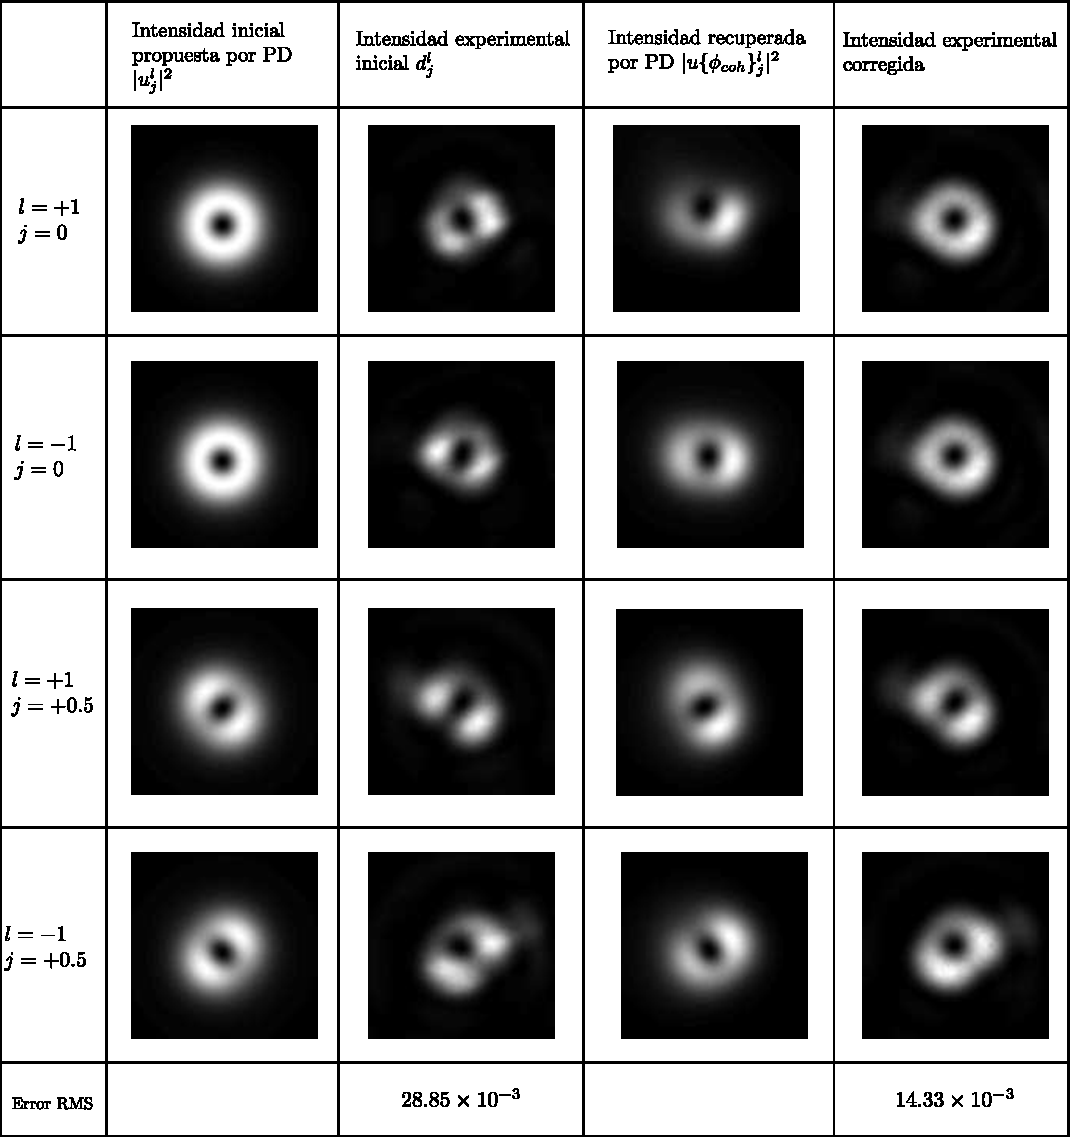
\includegraphics[width=\textwidth,keepaspectratio]{Caps/Imagenes/CorPD0.pdf}
  \caption[Corrección de OVs empleando PD coherente.]{Corrección de OVs empleando PD coherente. Las intensidades generadas por un sistema limitado por difracción con una modulación ideal $|u_j^l|^2$ son aproximadas a las mediciones experimentales $d_j^l$ mediante una fase $\phi_{coh}$ que es la diferencia entre ambas. A partir de la fase recuperada pueden corregirse las aberraciones presentes en $d_j^l$ y reducirse casi a la mitad el error con respecto a los OVs ideales.}
  \label{fig:corpd0}
\end{figure}

Para determinar si efectivamente hay una corrección de las aberraciones del sistema óptico y por tanto un aumento en la calidad de los OVs producidos, se tomó el error RMS promediado pixel a pixel entre la intensidad experimental inicial y la intensidad corregida con respecto a un OV producido por un sistema óptico limitado por difracción con modulación de fase ideal para cada diversidad (presentados en la fila inferior de la Fig. \ref{fig:corpd0}). Con esto se concluye que el error de la intensidad experimental corregida se reduce casi a la mitad con respecto a la intensidad inicial, por ende, efectivamente hemos corregido aberraciones del sistema óptico.\\

Podemos concluir que es posible recuperar las aberraciones que presentan los OVs a partir del empleo de PD coherente para OVs generados ``en línea'', y se pueden corregir las aberraciones mediante la superposición del inverso de la fase de las aberraciones en las máscaras de fase; esto se evidencia en una disminución del error entre los OVs corregidos y sus diversidades, con su ideal correspondiente. A continuación, aplicaremos las modificaciones de PD coherente (PD1 y PD2) que permiten recuperar $\phi_{coh}$ a partir de $\phi_{so}$ y $\phi_{slm}$. 
%También es importante recordar que los resultados son tomados a partir de una única fase para todas las diversidades y por ende como se esperaba, $\phi_{coh}$ representa la fase capaz de producir no sol


%Para el caso de PD coherente, Echeverri et al \cite{Echeverri2015} emplearon redes de difracción para la generación experimental de OVs.
%Al aplicar PD coherente a OVs buscamos encontrar un conjunto de aberraciones que caractericen el sistema óptico. Ahora bien, empleamos un conjunto de imágenes obtenidas experimentalmente que describan el comportamiento de los OVs ante diferentes OAMs y diversidades de Zernike. En este primer caso, se tiene un conjunto de imágenes experimentales, mostrado en la Fig.\ref{fig:cor_pd}, en donde se encuentran presente la aberración del sistema óptico en cada uno de los OVs. Ahora bien, siguiendo el esquema presentado en la sección \ref{sec:PD_coherente}, se empleó un conjunto de nuevo diversidades y desde ello se recuperaron las aberraciones presentes en los OVs. Con el conjunto de aberraciones puede entonces aplicarse una fase contraria a la SPM presentada al SLM y con ello, compensar las aberraciones del sistema. 
%
%\begin{figure}[!ht]
%  \centering
%    \includegraphics[scale=0.7]{Caps/Imagenes/CorPDcoherente.pdf}
%  \caption{Corrección de aberraciones en OVs con PD coherente.}
%  \label{fig:cor_pd}
%\end{figure}
%
%%De hecho, gracias a que se emplea un SLM es posible generar las diversidades de fase a partir de cualquier posible aberración, extendiendo el caso tradicional, en donde se empleaban desenfoques. A causa de la sensibilidad de los OVs ante ciertas aberraciones, además de añadir un grado de libertad a la función error, hay una mejora en la función error puesto que aun con una misma magnitud, puede conseguirse una deformación mayor en los OVs y por tanto un incremento en el error producido por función error y desde allí, mejorar el desempeño del GSA.
%Echeverri et al \cite{Echeverri2015} emplearon redes de difracción para la generación de sus OVs y por tanto, los OVs no presentan las aberraciones inducidas por el SLM puesto que este no necesariamente es sometido a modulaciones de fase de $2\pi$, de hecho, podría ser empleado en configuraciones de modulación de amplitud. Ahora bien, como fue propuesto en la sección \ref{sec:pd12} se puede emplear información adicional sobre el SLM y desde allí, reconocer qué aporte a las aberraciones del sistema proviene del SLM y qué aporte proviene del sistema óptico como tal. También se mostró anteriormente que la modulación del SLM repercute sobre las características de los OVs y que por tanto, si no se emplean redes de difracción, sino que el SLM se considera una SPP programable, entonces hay otras aberraciones que surgen en los OVs. \\
%
%
%%Ahora De aquí podemos inferir que PD funciona apropiadamente para casos de aberraciones en OVs que se generan por ejemplo, a través de redes de difracción pues en este caso no es tan relevante contar con modulaciones de fase cercanas a $2\pi$. 
%Ahora nuestro objetivo es poder obtener resultados similares en la corrección de OVs, pero sobre los OVs producidos por el sistema óptico cuando no se emplean redes de difracción, teniendo en cuenta que de por si, el SLM induce una aberración sobre el OVs. Corrigiendo con PD coherente los OVs obtenidos en la sección \ref{sec:vor_opt_expe} se obtuvieron los resultados mostrados en las Fig.\ref{fig:corpd0} y Fig.\ref{fig:fasepd0}. La primera figura muestra las intensidades que se obtuvieron, donde es claro que al corregir con PD coherente se mejora la calidad de los OVs experimentales. La segunda figura muestra los coeficientes y las fases que se obtuvieron para este caso, los coeficientes de Zernike comienzan en el 3 puesto que los tres primeros solo desplazan la fase, no repercuten en la forma del haz, también se presenta la fase real, que corresponde a los valores de modulación real que ve la luz, dados por el nivel de gris de cada uno de los valores de fase, es decir, Fig.\ref{fig:fasepd0} es igual a Fig.\ref{fig:fasepd0}, lo que las diferencia es que acorde a la curva de modulación los valores de fase pueden no necesariamente ser iguales.
%
%\begin{figure}[!ht]
%  \centering
%    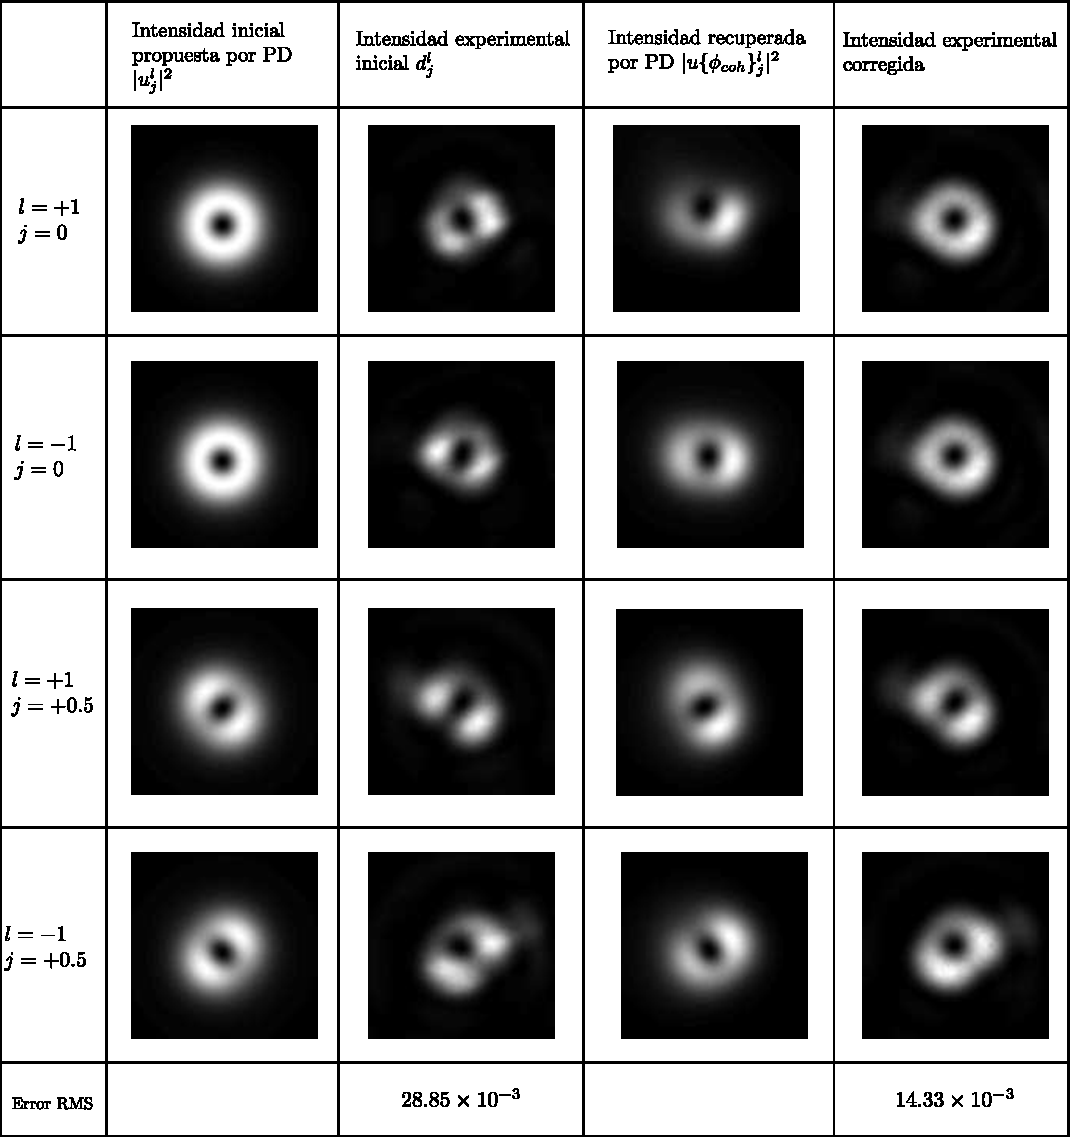
\includegraphics[width=\textwidth,keepaspectratio]{Caps/Imagenes/CorPD0.pdf}
%  \caption{Corrección de OVs empleando PD coherente.}
%  \label{fig:corpd0}
%\end{figure}
%
%\begin{figure}[!ht]
%  \centering
%    \includegraphics[width=\textwidth,keepaspectratio]{Caps/Imagenes/Fasepd0.pdf}
%  \caption{Fase obtenida con PD coherente. a)Magnitud e índices de las aberraciones en la base Zernike recuperado, b) fase por modulación real y c) fase ideal.}
%  \label{fig:fasepd0}
%\end{figure}
%
%Ahora apliquemos las variaciones sobre PD coherente a fin de poder determinar las aberraciones que provienen del SLM y del sistema óptico, para ello apelaremos a los conceptos de PD1 y PD2.



\section{Diversidad de fase como sensor de aberraciones por modulación}
\label{sec:cor_pd2}

%En capítulos anteriores, se planteó que la curva de modulación puede ser implementada en el algoritmo de PD y que con ellos se puede 
%Como fue planteado, cuando empleamos PD para recuperar las aberraciones causadas por la modulación del SLM, consideramos el resultado que genera un sistema óptico limitado por difracción y asumimos que ese es nuestro resultado experimental, es decir, suponemos que los OVs iniciales se encuentran aberrados exclusivamente por la modulación del SLM y a través de una modificación por el sistema óptico, recuperamos un OVs ideal. El resultado que sale de esto es entonces una máscara de fase tal que la aberración que es ocasionada por el SLM es corregida y por tanto esta corresponde a la aberración inducida por el SLM. Es importante notar que en este caso no se requiere de resultados de OVs experimentales, de hecho, el único elemento que proviene experimentalmente es la curva de modulación y aun antes de generar OVs pueden corregirse.\\
%
%La Fig.\ref{fig:corpd2} y la Fig.\ref{fig:fasepd2} muestran los resultados en intensidad y fase respectivamente obtenidos al emplear como entradas para el algoritmo de PD la CMR y OVs obtenidos en un sistema limitado por difracción. En este caso se muestra el resultado a OVs con carga topológica $\pm 1$ adicionando como diversidad de fase de Zernike de astigmatismo $Z_4$ en la magnitud correspondiente. El error RMS que se referencia en la figura corresponde al error RMS entre un OV producido por un sistema limitado por difracción con modulación ideal y la imagen en cuestión. Como es de esperar, se corregirán en los OVs experimentales las aberraciones que son ocasionadas por el SLM y por tanto, la aberración presente en los OVs experimentales son las inducidas por el sistema óptico. De la figura, también es claro que las correcciones efectuadas por PD2 mejoran la calidad de los OVs, esto se refleja en una disminución del error RMS de los OVs corregidos respecto a los generados experimentalmente.
%%Las imágenes que se encuentran dentro del recuadro verde corresponden a aquellas que se emplearon en PD, es decir, se comparan OVs generados por un sistema limitado por difracción con un SLM ideal con los que serían generado por un sistema limitado por difracción con el SLM real, nótese que en este caso, no se emplean resultados de OVs experimentales para PD, de hecho, el único elemento tomado experimentalmente es la curva de modulación. 
%%El error RMS que se referencia en la figura corresponde al error RMS entre un OV producido por un sistema limitado por difracción con modulación ideal y la imagen en cuestión. Como es de esperar, se corregirán en los OVs experimentales las aberraciones que son ocasionadas por el SLM y por tanto, la aberración presente en los OVs experimentales serán las inducidas por el sistema óptico. De la figura, también es claro que las correcciones efectuadas por PD2 mejoran la calidad de los OVs, esto se refleja en una disminución del error RMS de los OVs corregidos respecto a los generados por un sistema limitado por difracción.

Con respecto a las modificaciones sobre PD coherente, de la Sección \ref{sec:pd12}, recuperaremos $\phi_{slm}$ si empleamos PD2, es decir, a partir de la intensidad obtenida para un OV generado por una modulación de fase ideal y un sistema óptico limitado por difracción $|u_j^l|^2$, con la intensidad producida por un OV generado por la modulación de fase experimental con un sistema óptico limitado por difracción $|o_j^l|^2$. Si tomamos los resultados de la Sección \ref{sec:sim_vor_mod_exp} para $|o_j^l|^2$, podemos entonces obtener $\phi_{slm}$ a partir de PD coherente, como se muestra en la Fig. \ref{fig:corpd2}. \\

\begin{figure}[!ht]
  \centering
    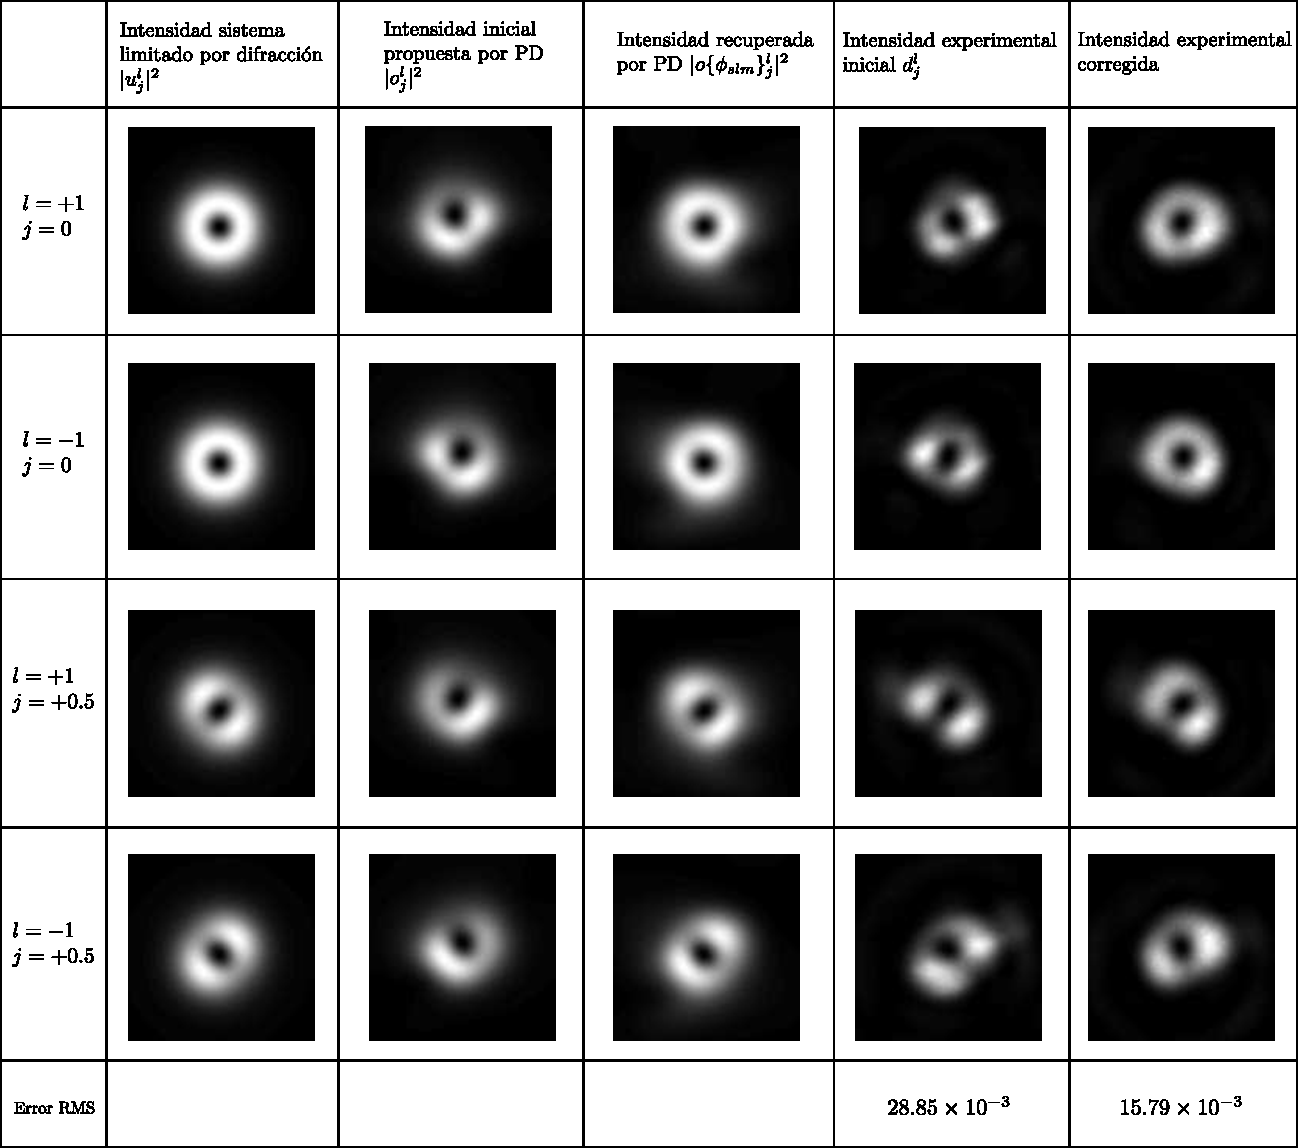
\includegraphics[width=\textwidth,keepaspectratio]{Caps/Imagenes/CorPD2.pdf}
  \caption[Corrección de OVs empleando PD2.]{Corrección de OVs empleando PD2. En este caso, suponemos que $|u_j^l|^2$ corresponde a la medida experimental de los OVs y que $|o_j^l|^2$ es el OVs que produce el sistema óptico, de forma que el sistema óptico en ambos casos es limitado por difracción ($\phi_{so}=0$) y por tanto, la aberración recuperada por PD coherente de acuerdo a la Eq. \ref{eqPDs} es $\phi_{coh} = \phi_{slm}$. Si se corrige la aberración encontrada, hay una disminución en el error RMS de los OVs corregidos respecto a los iniciales, cuando estos se comparan a OVs ideales.}
  \label{fig:corpd2}
\end{figure}


Se comienza suponiendo que $|u_j^l|^2$ es la intensidad medida, es decir, los OVs experimentales obtenidos son ideales, ahora se toma la intensidad $|o_j^l|^2$, y por medio del algoritmo de búsqueda de gradiente, se recupera una fase $\phi_{slm}$ que hace que $|o\{\phi_{slm}\}_j^l|^2$ sea similar a $|u_j^l|^2$, de forma que esta fase corresponde a la única diferencia posible entre $|u_j^l|^2$ y $|o_j^l|^2$, que es justamente la aberración de la modulación en fase. Si corregimos $\phi_{slm}$ en los OVs experimentales, se nota que la intensidad corregida presenta un menor error RMS promediado con respecto a un OV ideal, de forma que hay una corrección sobre $d_j^l$. Con respecto al caso de PD coherente, se esperaría que la disminución en el error RMS de la corrección con PD2 fuese menor que la corrección con PD coherente, dado que $\phi_{coh} = \phi_{slm}+\phi_{os}$ y si comparamos los errores RMS de dichos casos, efectivamente, PD coherente corrige en mejor medida (disminuye en mayor cantidad el error entre el OV corregido y el ideal) los OVs.\\

A partir de los resultados de PD2 podemos concluir que cuando corregimos los OVs para dos sistemas limitados por difracción en donde la única diferencia entre estos es la modulación experimental, podemos corregir aberraciones incluso antes de obtener resultados experimentales para los OVs (puesto que tanto $|u_j^l|^2$ como $|o_j^l|^2$ provienen de la simulación de un sistema limitado por difracción) y esta corrección se realiza sobre la aberración que produce la modulación experimental $\phi_{slm}$. El próximo paso es obtener $\phi_{so}$, para ello debemos recurrir al concepto de PD1, como se mostrará en la siguiente sección.
%
%\begin{figure}[!ht]
%  \centering
%    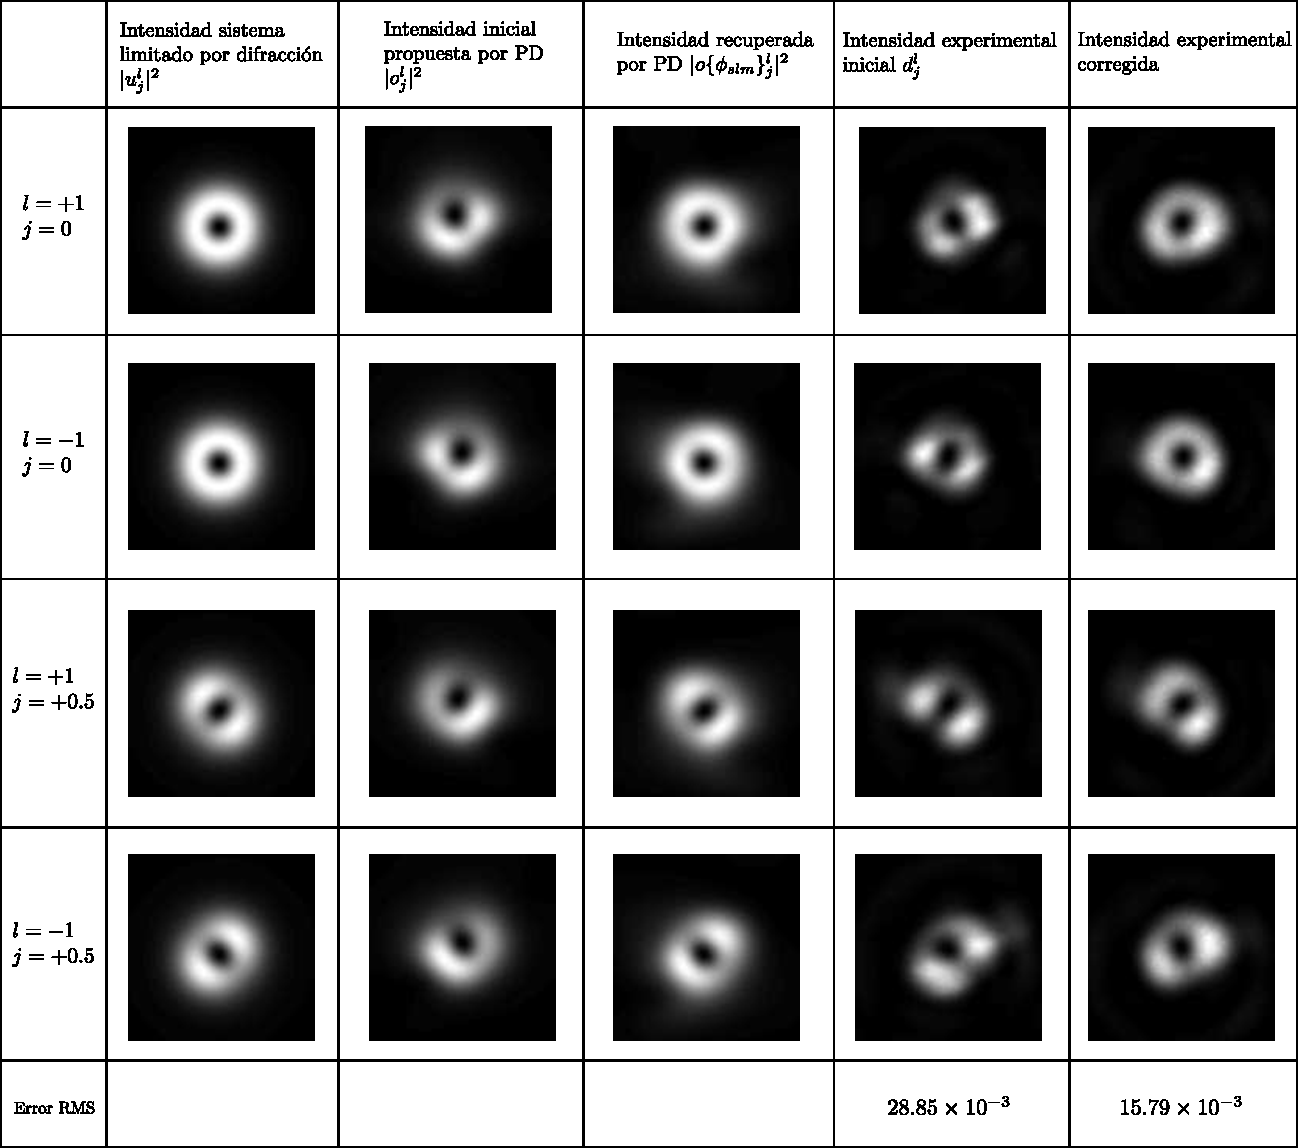
\includegraphics[width=\textwidth,keepaspectratio]{Caps/Imagenes/CorPD2.pdf}
%  \caption{Corrección de OVs empleando PD2.}
%  \label{fig:corpd2}
%\end{figure}
%
%\begin{figure}[!ht]
%  \centering
%    \includegraphics[width=\textwidth,keepaspectratio]{Caps/Imagenes/Fasepd2.pdf}
%  \caption{Fase recuperada empleando PD como sensor de aberraciones producidas por el SLM. a) Magnitud y coeficientes de Zernike, b) fase real y c) fase ideal.}
%  \label{fig:fasepd2}
%\end{figure}

%También hay que notar que si bien se aproximan los OVs propuestos en PD2, no todos obtienen el mismo valor de error, esto es debido a que se recuperan las aberraciones del SLM como una combinación de aberraciones que minimizan el error producido por el conjunto entero de las imágenes y por tanto, si bien como conjunto cumplen un mínimo de la función error, esto no quiere decir que localmente cada imagen cumple un valor mínimo de la función error.

\section{Diversidad de fase como sensor de aberraciones del sistema óptico}
\label{sec:cor_pd1}

%De manera similar al caso de PD2 podemos modificar PD coherente para obtener las aberraciones propias del sistema óptico, para ello, hay que incorporar la CMR a los OVs producidos por un sistema limitado por difracción. Si suponemos que nuestro OV ideal es aquel que se genera en un sistema limitado por difracción, pero que posee la modulación del SLM e intentamos recuperar las aberraciones presentes en los resultados experimentales, al considerar las aberraciones del SLM intrínsecas al sistema limitado por difracción, obtendremos las aberraciones que son propias del sistema óptico independiente del SLM. Los resultados de este caso se muestran en la Fig.\ref{fig:corpd1} para la intensidad y en la Fig.\ref{fig:fasepd1} para la fase, el error RMS corresponde a la diferencia entre la imagen y la producida por un sistema limitado por difracción. Se observa que de manera similar al caso anterior, se mejora la calidad de los OVs luego de su corrección, lo que nos indica que eventualmente estamos corrigiendo las aberraciones del sistema óptico.\\

%Si ahora comparamos el error RMS de obtenido con cada una de las correcciones, puede apreciarse que la mejor corresponde a la que fue realizada con PD coherente, seguida por PD para la detección de aberraciones causadas por el sistema óptico y finalmente, PD para la detección de aberraciones del SLM, de aquí podemos concluir que la mayor parte de las aberraciones corresponden a las causadas por el sistema óptico. Finalmente, se aplicó PD para detectar la aberración del sistema óptico a un sistema con una aberración similar al caso de \ref{sec:div_coh} como se muestra en la Fig.\ref{fig:corpdcoherente1}, en donde similar a la Fig.\ref{fig:cor_pd} pueden corregirse las aberraciones causadas por el sistema óptico, aunque puesto que no corregimos aquellas aberraciones ocasionadas por el SLM, cualitativamente podríamos concluir que es más mala.

De la Sección \ref{sec:pd12}, recuperamos $\phi_{so}$, que es la aberración causada por el sistema óptico independiente de la modulación del SLM si empleamos PD1, por tanto, a partir de $|o_j^l|^2$ y $d_j^l$  en PD coherente se obtiene $\phi_{so}$. En este caso, $|o_j^l|^2$ y $d_j^l$ contienen información de la modulación experimental del SLM y en ellas solo difiere la propagación por el sistema óptico, de forma que la aberración $\phi_{coh} = \phi_{so}$. Los resultados de PD1 se muestran en la Fig. \ref{fig:corpd1}, para este caso, $|o_j^l|^2$ y $d_j^l$ son conocidos puesto que se han empleado en PD coherente y en PD1, lo que se debe hacer es tomar estos como las entradas de PD coherente y el objetivo del algoritmo de búsqueda de gradiente es encontrar una fase $\phi_{so}$ tal que la diferencia entre $|o_j^l|^2$ y $d_j^l$ sea mínima (es decir, que el funcional $L$ es un mínimo). La intensidad $|o\{\phi_{so}\}_j^l|^2$ corresponde a la generada por el sistema óptico cuando se obtiene la fase $\phi_{so}$ final, de manera que si se corrigen los OVs obtenidos experimentalmente, de manera similar a los casos anteriores, hay una disminución del error RMS respecto a un OV ideal. Al igual que en PD2, se tiene que la reducción en el error RMS es menor que la producida por PD coherente como era de esperar. Ahora, si comparamos el error RMS obtenido para las correcciones con PD1 y PD2, su magnitud es similar, lo que nos indica que las aberraciones a causa de la modulación tienen una magnitud similar a las del sistema óptico. Los resultados de los errores y las correcciones de las diferentes versiones de PD se resumen en la Tabla \ref{tab:corpd}.\\

\begin{figure}[!ht]
  \centering
    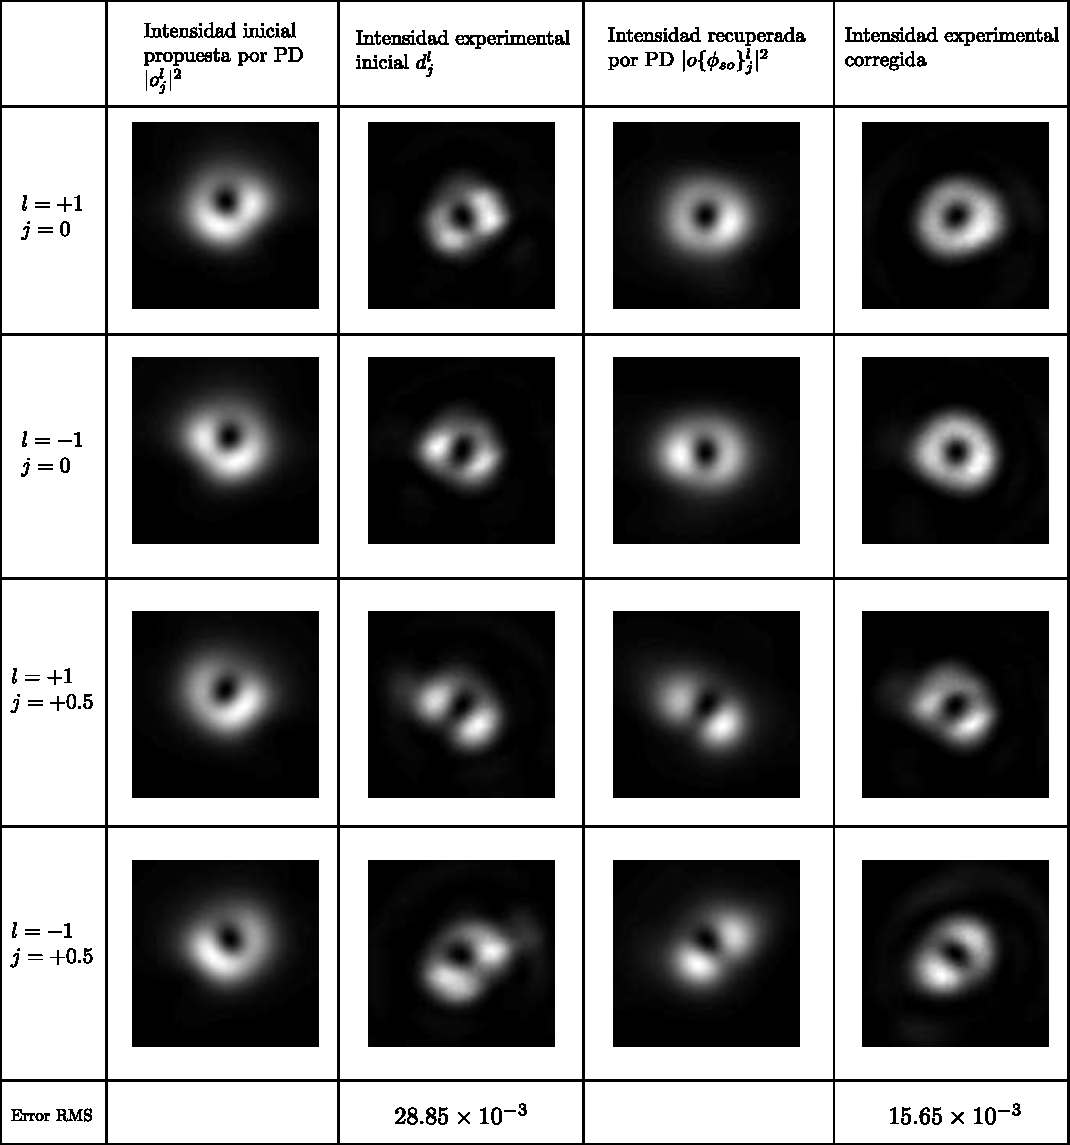
\includegraphics[width=\textwidth,keepaspectratio]{Caps/Imagenes/CorPD1.pdf}
  \caption[Corrección de OVs empleando PD1.]{Corrección de OVs empleando PD1. En este caso, se toma la intensidad experimental de los OVs experimentales $d_j^l$ y los OVs generados por un sistema óptico limitado por difracción con modulación experimental $|o_j^l|^2$ de forma que en ambos casos se ha considerado la aberración causada por la modulación de fase, y por tanto, la aberración recuperada por PD coherente es $\phi_{coh} = \phi_{so}$. Si se corrige la aberración encontrada, hay una disminución en el error RMS de los OVs corregidos respecto a los iniciales, cuando estos se comparan con OVs ideales}
  \label{fig:corpd1}
\end{figure}

\begin{table}[!ht]
\centering
\begin{tabular}{|c|c|}
\hline 
  & Error RMS \\ 
\hline 
OV ideal - Experimental inicial & $28.85\times 10^{-3}$ \\ 
\hline 
OV ideal - Corrección PD coherente & $14.33\times 10^{-3}$ \\ 
\hline 
OV ideal - Correccion PD1 & $15.65\times 10^{-3}$ \\ 
\hline 
OV ideal - Corrección PD2 & $15.79\times 10^{-3}$ \\ 
\hline 
\end{tabular} 
\caption{Resultados del error RMS para cada una de las correcciones con PD.}
\label{tab:corpd}
\end{table}

Ahora, queremos comprobar que como se planteó en la Sección \ref{sec:pd12}, las aberraciones cumplen la Eq. \ref{eqPDs}; esto puede demostrarse si a partir de las aberraciones obtenidas por PD coherente $\phi_{coh}$ y las del sistema óptico $\phi_{so}$ podemos obtener las aberraciones que son causadas por la modulación de fase experimental $\phi_{slm}$, de modo que,

\begin{equation}
\label{eqR1}
\phi_{slm} = \phi_{coh}-\phi_{so},
\end{equation}

esto se muestra en la Fig. \ref{fig:fases}. Con $\phi_{coh}$ obtenido en la Sección \ref{sec:cor_div_coh} (Fig. \ref{fig:fases}(a)) y $\phi_{os}$ obtenido previamente (Fig. \ref{fig:fases}(b)) podemos obtener un $\phi'_{slm}$ (Fig. \ref{fig:fases}(d)) que representa la aberración debida a la modulación del SLM obtenida a partir de $\phi_{coh}$ y $\phi_{so}$, empleando de la Eq. \ref{eqR1}, de hecho, $\phi_{slm}$ fue determinado anteriormente con PD2 (Fig. \ref{fig:fases}(c)), por ende, podemos evaluar la correspondencia entre $\phi_{slm}$ y $\phi'_{slm}$. Para este último propósito, se comparó $\phi'_{slm}$ y $\phi_{slm}$ con un frente de onda plano, de forma que se obtiene la magnitud de la aberración del frente de onda, como se muestra en la Tabla \ref{tab:compfases}. Se obtuvo que la magnitud de $\phi_{slm}$ y $\phi'_{slm}$ respecto a un frente de onda plano es semejante y es de esperar que entre ambos haya correspondencia, para lo cual se realizó una diferencia en los frentes de onda y se obtuvo un error de $0.87 \lambda$ mostrando que efectivamente hay correlato entre $\phi_{slm}$ y $\phi'_{slm}$.

\begin{figure}[!ht]
  \centering
    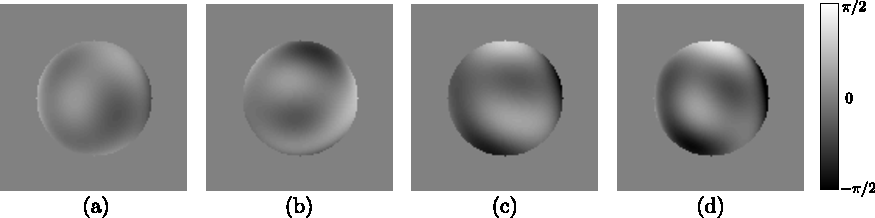
\includegraphics[width=\textwidth,keepaspectratio]{Caps/Imagenes/fases.pdf}
  \caption[Comparación de las aberraciones obtenidas con PD coherente, PD1 y PD2.]{Comparación de las aberraciones obtenidas para cada una de las modificaciones de PD coherente. (a) Aberración obtenida con PD coherente $\phi_{coh}$, (b) aberración obtenida con PD1 $\phi_{so}$, (c) aberración obtenida con PD2 $\phi_{slm}$ y (d) $\phi '_{slm}$ obtenida a través de la diferencia entre $\phi_{coh}$ y $\phi_{so}$.}
  \label{fig:fases}
\end{figure}

\begin{table}[!ht]
\centering
\begin{tabular}{|c|c|}
\hline 
Comparación & Error RMS [$\lambda$] \\ 
\hline 
$\phi_{slm}$ - Frente de onda plano & $66.21\times 10^{-3} $ \\ 
\hline 
$\phi'_{slm}$ - Frente de onda plano & $66.31\times 10^{-3}$ \\ 
\hline 
$\phi_{slm}$ - $\phi'_{slm}$ & $0.87 \times 10^{-3}$ \\ 
\hline 
\end{tabular}
\caption{Comparación de los frentes de onda recuperados a través de PD coherente, PD1 y PD2.}
\label{tab:compfases}
\end{table}
%
Finalmente, aunque aquí no fuera mostrado, con el mismo procedimiento realizado pueden corregirse aberraciones en OVs cargas topológicas $l$ diferentes a $\pm 1$, en la Fig. \ref{fig:coroam2} se muestra la corrección que se obtuvo para un OV con $l=-2$.

\begin{figure}[!ht]
  \centering
    \includegraphics[width=\textwidth,keepaspectratio]{Caps/Imagenes/corOAM2.pdf}
  \caption[Corrección de un OV con $l=-2$.]{Corrección del OV con $l=-2$ en cada una de las versiones de PD coherente. (a) OV experimental inicial, (b) OV experimental cuando se corrige $\phi_{coh}$, (c) OV experimental cuando se corrige $\phi_{so}$ y (d) OV experimental cuando se corrige $\phi_{slm}$}.
  \label{fig:coroam2}
\end{figure}
%\include{Caps/Resultados2}
%
\chapter{Conclusiones y trabajo futuro}
\label{cap:conclusiones}

%PD 
%Aquí se ha planteado un modelo basado en diversidad
%
%%Se planteó a pepe y se comprobó que 2+2 = pepepepepez Kappa
%
%%El objetivo de este proyecto
%
%Se propuso un método novedoso para la caracterización de aberraciones en sistemas ópticos basado en el uso de OVs para mejorar la respuesta de la fase recuperada. También se mostró que el método funciona para un grado considerable de aberraciones.
%
%A partir de PD coherente, se propuso una modificación de forma tal que es posible identificar aberraciones no solo de sistemas ópticos, si no que puede emplearse para caracterizar la fase de SLMs, esto basados en los datos experimentales obtenidos del SLM
%además de esto, puede emplearse como un método complementario al PD.

Para el SLM LC-2002 concluimos que si bien posee estados de modulación de $2\pi$ en fase, estos no necesariamente son los mejores estados para la generación de OVs, puede ser mejor emplear un estado que posea una menor modulación en fase, su comportamiento sea \textit{suave}, y que la tramtancia tenga una variación de alrededor de $30\%$ para todos los niveles de gris. A partir del conocimiento de esta curva de modulación se implementó un algoritmo que permite describir OVs con información experimental del SLM.\\


Con base en los algoritmos de PD desarrollados del Grupo de Óptica Aplicada de la Universidad EAFIT, se desarrollaron dos nuevas posibilidades para sensar aberraciones a través de PD. La primera de ellas PD1, permite obtener las aberraciones causadas por un sistema óptico que genera OVs a partir de un SLM, ya que considera las aberraciones causadas por la modulación de fase en los OVs que obtiene como solución a las aberraciones. Por otro lado, PD2 permite recuperar las aberraciones que son causadas por la modulación en fase del SLM, gracias a que considera un sistema óptico limitado por difracción, en donde la única aberración que pueden presentar los OVs son aquellas que sean causada por la modulación en fase. Una de sus  principales características es que permite predecir aberraciones incluso antes de que se generen OVs experimentales.\\

La implementación de PD1 y PD2 a OVs experimentales demuestra que PD1 como PD2 corrigen una parte de las aberraciones, manifestándose esto en una mejor en la calidad de los OVs. Sin embargo, la corrección brindada por PD coherente contiene información de los resultados obtenidos con PD1 y PD2.\\

Con los resultados de fase encontrados se determinó que a partir de las aberraciones recuperadas con PD coherente, PD1 y PD2 efectivamente tienen correspondencia, debido a que a partir de el resultado de PD coherente y PD1, pudo recuperarse satisfactoriamente las aberraciones obtenidas a partir de PD2.\\

Como trabajo futuro se propone:

\begin{itemize}
\item Modificar los algoritmos de PD coherente para que en este puedan emplearse redes de difracción.
\item Emplear PD2 para como sensor de aberraciones de modulación en SLMs cuya modulación en fase difiera por la linealidad y \textit{suavidad} de la curva para determinar el efecto de estas características en la generación de OVs.
\end{itemize} 
%

\addcontentsline{toc}{chapter}{Referencias}
\bibliographystyle{unsrt}
%\bibliography{ReferenciasPG,RefJefe}
\bibliography{ReferenciasPG}

%\appendix
%\chapter*{Anexos}
%\newpage
%\includepdf[pages={1,2,3,4}]{Coherent_illumination_PD.pdf}
\end{document}